% !TeX spellcheck = en_US
% !TEX TS-program = xelatex 
\documentclass[a4paper, 12pt, twoside, titlepage]{book}
\usepackage{./multimedia-book-style} %custom style with preamble

\sloppy % \textnp{margin बाहिर गएकाे text लाई right ragged गर्ने।}


% \includeonly {
%./chapters/chapter-1},
%{./chapters/chapter-2}, 
%{./chapters/chapter-3}, 
%{./chapters/chapter-4},
%{./chapters/chapter-5},
%{./chapters/chapter-6},
%{./chapters/chapter-7},
%{./chapters/chapter-8},
%{./chapters/chapter-9},
%}

\begin{document}


\title{\huge {Multimedia Application}}
\author{Jeevan Poudel}
\date{2021}


%@@@@@@@@@@@@@@@@@@@@@@@@@@@@@@@@@@@@
%				    				@
%         Front Matter		    	@
%				    				@
%@@@@@@@@@@@@@@@@@@@@@@@@@@@@@@@@@@@@

\frontmatter
	

\includepdf[pages={2}, scale=1.07]{./cover/multimedia-application}\thispagestyle{empty}%cover page inclusion

\begin{titlepage}
	\centering


	{\scshape\LARGE Purbanchal University, Nepal \par}
\vspace{0.5cm}
\vspace*{\baselineskip} % White space at the top of the page

\rule{\textwidth}{1.6pt}\vspace*{-\baselineskip}\vspace*{2pt} % Thick horizontal rule
\rule{\textwidth}{0.4pt} % Thin horizontal rule

\vspace{0.75\baselineskip} % Whitespace above the title

	{\huge\bfseries Multimedia Application (BCA452CO)\par}
	
	\vspace{0.75\baselineskip} % Whitespace below the title
	
	\rule{\textwidth}{0.4pt}\vspace*{-\baselineskip}\vspace{3.2pt} % Thin horizontal rule
	\rule{\textwidth}{1.6pt} % Thick horizontal rule
	
	\vspace{2\baselineskip} % Whitespace after the title block
	
	{\normalsize \bfseries (Compiled Notes)}
	
	\vspace{2cm}
	
	{\Large\scshape BCA-VIII \par}


	\vfill

{\Huge\scshape ~{Jeevan Poudel}\par}


	\vfill



\vspace{0.3\baselineskip} 
% Bottom of the page
	{\large ~{\textnp{श्री गोमेन्द्र बहुमुखी महाविद्यालय \vspace*{0.1cm}\\ विर्तामोड, झापा \vspace*{0.1cm}\\ चैत ६, २०७७}\vspace*{0.1cm} \\(2021)} \par} 
	
\newpage
\vspace*{\fill}
\thispagestyle{empty}

\newpage
\vspace*{\fill}
\thispagestyle{empty}
\begin{center}
	\begin{nepali}
			{\large {याे पाठ्‍य सामग्री तयार पार्न साथ, सहयोग र हाैसला प्रदान गर्नुहुने आदरणीय गुरु श्री सिद्धार्थ कायस्था र मेरा सबै साथीहरुप्रति हार्दिक आभार प्रकट गर्दछु।}}
	\end{nepali}
\end{center}
\vspace*{\fill}

\end{titlepage}
\thispagestyle{empty}
\phantomsection


\setcounter{secnumdepth}{5} %set section depth, starts with 0, default:3, 
\setcounter{tocdepth}{3} %set TOC depth, default:2, 



\tableofcontents \newpage\thispagestyle{empty}

\listoffigures \addcontentsline{toc}{chapter}{\listfigurename} \newpage \thispagestyle{empty}

\listoftables\addcontentsline{toc}{chapter}{List of Tables} \newpage \thispagestyle{empty}

%@@@@@@@@@@@@@@@@@@@@@@@@@@@@@@@@@@@@
%									@
%			Main Matter				@
%									@
%@@@@@@@@@@@@@@@@@@@@@@@@@@@@@@@@@@@@

\mainmatter
%%%%%%%%%%%%%%%%%%%%%%%%%%%%%%%%%%%%%%%%%%%
\chapter{Multimedia System}

\section{Introduction, Concept and Structure}
\subsection{Introduction}
The word multimedia is composed of two parts: the prefix \emph{multi} and the root \emph{media}. The prefix \emph{multi} comes from the Latin word \emph{multus}, which means ``numerous".

The root \emph{media} is the plural form of the Latin word \emph{medium}. \\

In general, \textit{medium} is a means for distribution and presentation of
information., Examples of a medium are \textit{text}, \textit{graphics}, \textit{speech} and \textit{music}.


%https://www1.udel.edu/edtech/multimedia/index.html
\noindent Multimedia is the use of a computer to present and combine text, graphics, audio, and video with links and tools that let the user navigate, interact, create, and communicate. 

This definition contains four components essential to multimedia. 
\begin{enumerate}
	\item First, there must be a computer to coordinate what we see and hear, and to interact with.
	\item Second, there must be links that connect the information. 
	\item Third, there must be navigational tools that let us traverse the web of connected information.
	\item Finally, there must be ways for us to gather, process, and communicate our own information and ideas.
\end{enumerate}

 If one of these components is missing, we do not have multimedia. For example:
 \begin{itemize}
 	\item If we have no computer to provide interactivity, we have mixed media, not multimedia. 
 	\item If there are no links to provide a sense of structure and dimension, we have a bookshelf, not multimedia. 
 	\item If there are no navigational tools to let us decide the course of action, we have a movie, not multimedia. 
 	\item If we cannot create and contribute our own ideas, we have a television, not multimedia.
 \end{itemize}

\subsection*{Multimedia Applications}
Examples of Multimedia Applications include:

\begin{multicols}{2}
\begin{itemize}
	\item World Wide Web
	\item Animation
	\item 3D Mapping
	\item Video-on-demand
	\item Interactive TV
	\item Computer Games
	\item Virtual reality
	\item Digital video editing and production systems
	\item Image processing
	\item Voice recognition
	\item Augmented reality
\end{itemize}
\end{multicols}
\subsection{Concept}
Multimedia can have many definitions these include:

\subsubsection*{A computer system perspective definition}
Multimedia means that computer information can be
represented through audio, video, and animation in addition to
traditional media (i.e., text, graphics/drawings, images).


\subsubsection*{General Definition}
Multimedia is the field concerned with the computer
controlled integration of text, graphics, drawings, still and
moving images (Video), animation, audio, and any other
media where every type of information can be represented,
stored, transmitted and processed digitally.

\subsection{Structure}
Figure {\ref{fig:multimedia-structure}} shows the main fields of multimedia systems.

%@@@@@@@@@@@@@@@@@@@@@@@@@@@@@@@@@@@@
%									@
%			FIGURE					@
%									@
%@@@@@@@@@@@@@@@@@@@@@@@@@@@@@@@@@@@@
		
\begin{figure}[H]
	\centering
	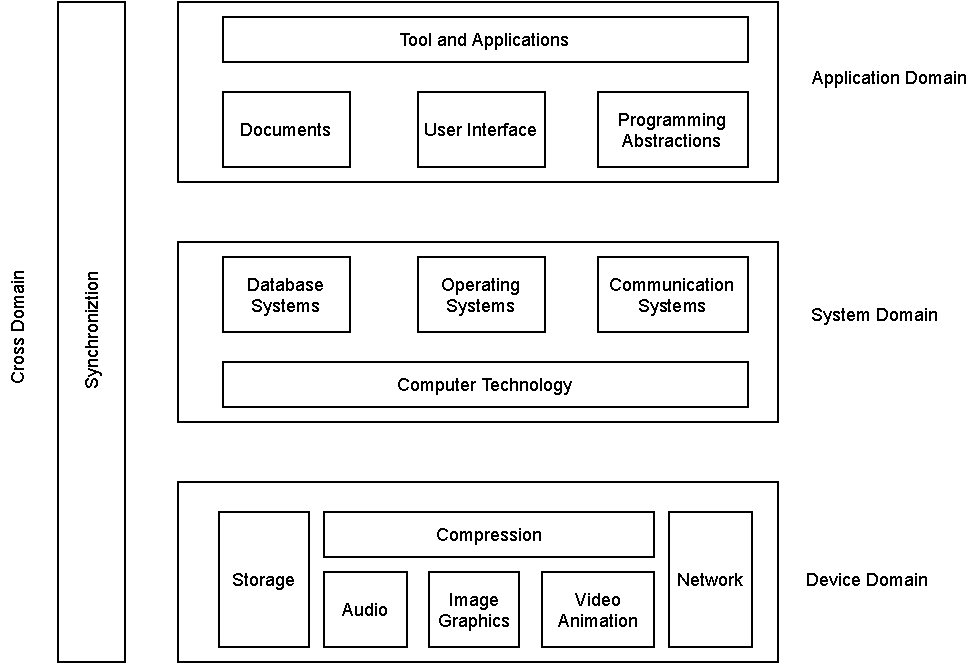
\includegraphics[width=\textwidth]{multimedia-structure}
	\caption{Main fields of multimedia systems.}\label{fig:multimedia-structure}
\end{figure}

\noindent The following areas can be distinguished:

\subsubsection*{Device Domain}
	Basic concepts for the processing of \textit{digital audio} and \textit{video} data are based
	on digital signal processing. Different methods for the	processing of \textit{image}, \textit{graphics} and \textit{animation} are included.
	
\subsubsection*{System Domain}
	The interface between the device domain and the system domain is specified
	by the \textit{computer technology}. To utilize the device domain, several system services are needed. Basically, three services exist. These services are mostly implemented in software:
		\begin{itemize}
			\item The \textit{operating system} serves as an interface between computer hardware/system software and all other software components.
			
			\item The \textit{database system }allows structured access to data and a management of large databases.
			
			\item The \textit{communication system} is responsible for data transmission according to the timing and reliability requirements of the networked multimedia application.
		\end{itemize}
	
	
\subsubsection*{Application Domain}
	
	The services of the system domain are offered to the application domain through proper programming abstractions.
	
	Another application domain is \textit{document handling}. A document consists of a set of structured information, represented in different media, and generated or recorded at the time of presentation.
	
	Many functions of document handling and other applications are accessible and presented to the user through a \textit{user interface}.
	
\subsubsection*{Cross Domain}
Some aspects, such as synchronization aspects, are difficult to locate in one or two components or domains. The reason is that \textit{synchronization}, being the temporal relationship among various media, relates to many components across all domains.


\section{Media Aspect Properties}
Media can be classified with respect to different criteria as follows:
\begin{multicols}{2}
	\begin{itemize}
	\item perception media 
	\item representation media
	\item presentation media
	\item storage media
	\item transmission media
	\item information exchange media
	\end{itemize}
\end{multicols}


\subsection{Perception Media}
Perception media refers to the nature of information perceived by humans. The question to ask here is: \emph{How do humans perceive information}? The answer is that the perception of information occurs mostly through seeing or hearing the information.

We distinguish primarily between what we see and what we hear. 
\begin{itemize}
	\item \textit{Auditory media} include music, sound, and voice. 
	\item \textit{Visual media} include text, graphics, and still and moving pictures.
\end{itemize}


\subsection{Representation Media}
The term representation media refers to how information is represented internally
to the computer. The question to ask here
is: \emph{How is information encoded in the computer?} The
answer is that various formats are used to represent media information in a computer. There are several options:

\begin{itemize}
\item A text character is coded in \gls{ascii} or \gls{ebcdic} code.
\item Graphics are encoded using \gls{gks} graphics standard.
\item An audio stream can be represented using \gls{pcm}
\item An image is in \gls{jpeg} format.
\item A combined audio-video sequence is stored in the computer in various TV standards (e.g., \gls{pal}, or \gls{ntsc}, or in \gls{mpeg} format).
\end{itemize}

\subsection{Presentation Media}
Presentation media refers to the physical means used by systems to reproduce information for humans. The question to ask here is: \emph{Which medium is used to output information
from the computer or input in the computer?}

We distinguish primarily between output and input media:
\begin{itemize}
	\item \textit{output media}: paper, computer monitors, and loudspeakers, etc.
	\item \textit{input media}: keyboards, cameras, and microphones, etc.
\end{itemize}


\subsection{Storage Media}
Storage media refers to various physical
means for storing computer data, such as magnetic tapes, magnetic disks, or digital
optical disks. However, data storage is not limited to the components available in a
computer, which means that paper is also a storage medium. The question to
ask here is: \emph{Where is information stored?} Example of storage media includes: \textit{Hard disk}, \textit{\gls{cd}}, \textit{\gls{usb} flash drive}\footnote{\textnp{बाेलीचालीकाे भाषामा पेन ड्राइभ (pen drive) पनि भनिन्छ}}, etc. 

\subsection{Transmission Media}
Transmission media refers to the physical media. The question to ask here is:
\emph{Which medium is used to transmit data?} The answer is that information is transmitted over networks, cables such as fiber or coaxial as well as free airspace transmission for wireless transmission.

\subsection{Information Exchange Media}
Information exchange media includes all data media used to transport information,
e.g., all storage and transmission media. The question to ask here is: \emph{Which data
medium is used to exchange information between different locations?}

For example, information can be exchanged by storing it on a removable medium
and transporting the medium from one location to another. These storage media include
microfilms, paper, and USBs, etc.

\section{Definition of Multimedia System}
A Multimedia System is a system capable of processing multimedia data and applications. A Multimedia System is characterized by the processing, storage, generation, manipulation and interpretation of Multimedia
information.


Characteristics of Multimedia System:

\begin{itemize}
	\item They must be computer-controlled.
	\item They are integrated.
	\item They must support media independence.
	\item And lastly, they need to handle discrete and continuous media.
\end{itemize}

\subsection{Discrete and Continuous Media}
If the application uses both discrete and continuous media then it is called multimedia. This means that a multimedia application should process at least one discrete and one continuous medium. A word processor with embedded graphics is not a multimedia application.

\subsection{Independent Media}
Media should not be tightly coupled together. They must be independent for example, digital audio and computer available text can be combined for the purpose of presentation. 

\subsection{Computer-Controlled Systems}
The independence of media creates a way to combine media for presentation. For this purpose, the computer is the ideal tool. The system can be optionally programmed by a programmer. The simple video recording and playback of media is a system such as video recorder is not sufficient to meet the requirements for computer controlled systems. 

\subsection{Integration}
Computer-controlled independent media streams can be integrated to form a global system so that, together, they provide a certain function. A word processor
that supports text, spreadsheets, and graphics does not meet the integration criterion
unless it allows program-supported references between the data. 

\section{Traditional Data Stream Characteristics}
Distributed networked multimedia systems transmit both discrete and continuous
media streams. In a digital system, information is split
into units (packets) before it is transmitted. These packets are sent by one system component (the \textit{source}) and received by another one (the \textit{sink}). Source and sink can reside on different computers. A data stream consists of a (temporal) sequence of packets. 

Packets can carry information from continuous and discrete media. 
\begin{itemize}
	\item Continuous medium: \textit{transmission of voice in a telephone system}
	\item Discrete medium : \textit{transmission of text file}
\end{itemize}


When we transmit information originating from various media, we obtain data
streams that have very different characteristics. The attributes 
\begin{multicols}{3}
\begin{enumerate}[label=\alph*)]
	\item asynchronous
	\item synchronous and 
	\item isochronous
\end{enumerate}
\end{multicols}


 are traditionally used in the field of telecommunications to describe the characteristics of a data transmission.


\subsection{Asynchronous Transmission Mode}
A communication is called asynchronous if a
sender and receiver do not need to coordinate before data can be transmitted. 
\begin{itemize}
	\item In asynchronous transmission, the transmission may start at any given instant.
	\item The bit synchronization that determines the start of each bit is provided by two independent clocks on both sender and receiver.
	\item Example: ASCII terminals attached to host computers. Whenever a character is pressed, a sequence of bits is generated and sent to the computer interface along with character.
	\item A special signal called \textit{start} signal precedes the information bits.
	\item Another special signal called \textit{stop} signal follows the last information bit.
\end{itemize}

\subsection{Synchronous Transmission Mode}
The synchronous transmission mode defines a maximum end-to-end delay for each packet of a data stream. This upper bound will never be violated.

In synchronous transmission, transmission begins when the clock signal is matched with the receiver.


\subsection{Isochronous Transmission Mode}
The isochronous transmission mode defines, besides a maximum end-to-end delay for each packet of a data stream, a minimum end-to-end delay.
\begin{itemize}
	\item This mode is a form of data transmission in which individual characters are only separated by a whole number of bit-length intervals. 
	\item For example, an end-to-end network connection is said to be isochronous if the bit rate over the connection is guaranteed and if the value of the delay \textit{jitter} is also guaranteed and small.
\end{itemize}

\section{Data Stream Characteristics For Continuous Media}
Following are the data stream characteristics that relate to any audio/video data transfer in a multimedia system (multimedia data streams).
\begin{itemize}
	\item The time interval between a complete transmission of consecutive packets.
	\item Variation of consecutive packet amount.
	\item Contiguous packets.
\end{itemize}

\subsection{The Time Interval Between a Complete Transmission of Consecutive Packets}
The first property of data streams relates to the time intervals between fully completed transmissions of consecutive information units or packets. Based on the moment
in which the packets become ready, we distinguish between the following variants:

\subsubsection{Strongly Periodic Data Stream}
\begin{itemize}
	\item When the time interval between neighboring packets is constant, then this data
	stream is called a \textit{strongly periodic} data stream.
	\item This also means that there is minimal jitter—ideally zero.
	\item Example: PCM-encoded voice in telephone systems.
\end{itemize}

 Figure {\ref{fig:strongly-periodic}} illustrates strongly periodic data stream.

%@@@@@@@@@@@@@@@@@@@@@@@@@@@@@@@@@@@@
%									@
%			FIGURE					@
%									@
%@@@@@@@@@@@@@@@@@@@@@@@@@@@@@@@@@@@@
\begin{figure}[ht]
\centering
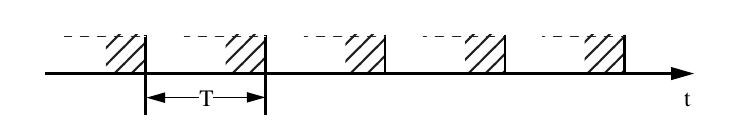
\includegraphics[width=\textwidth]{strongly-periodic}
\caption[Strongly periodic data stream]{Strongly periodic data stream; time intervals have the same duration between consecutive packets.}\label{fig:strongly-periodic}
\end{figure}

\subsubsection{Weakly Periodic Data Stream}
The duration of the time intervals between neighboring packets is often described
as a \textit{function with finite period duration}. However, this time interval is not constant between neighboring packets. The data stream is called \textit{weakly periodic}. The case is shown in Figure {\ref{fig:weakly-periodic}}.

%@@@@@@@@@@@@@@@@@@@@@@@@@@@@@@@@@@@@
%									@
%			FIGURE					@
%									@
%@@@@@@@@@@@@@@@@@@@@@@@@@@@@@@@@@@@@
\begin{figure}[ht]
	\centering
	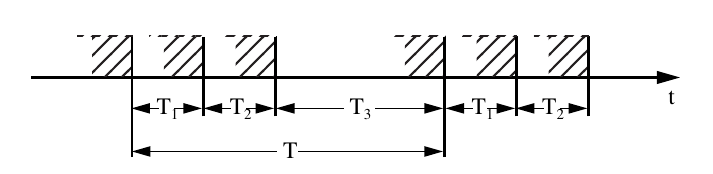
\includegraphics[width=\textwidth]{weakly-periodic}
	\caption[Weakly periodic data stream]{Weakly periodic data stream; time intervals between consecutive packets are periodic.}\label{fig:weakly-periodic}
\end{figure}

\subsubsection{Aperiodic Data Stream}
All other transmission options are called aperiodic data streams  (excluding strongly and weakly data stream), which relates to
the sequence of time interval duration, as shown in Figure {\ref{fig:aperiodic}}.

%@@@@@@@@@@@@@@@@@@@@@@@@@@@@@@@@@@@@
%									@
%			FIGURE					@
%									@
%@@@@@@@@@@@@@@@@@@@@@@@@@@@@@@@@@@@@
\begin{figure}[hb!]
	\centering
	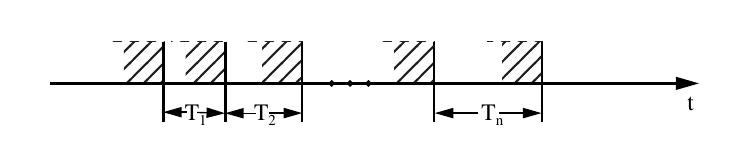
\includegraphics[width=\textwidth]{aperiodic}
	\caption[Aperiodic data stream]{Aperiodic data stream; the time interval sequence is neither constant nor weakly periodic.}\label{fig:aperiodic}
\end{figure}

An example of an aperiodic data stream is a multimedia conference application
with a common screen window. Often, the status (left button pressed) and the current
coordinates of the mouse moved by another user have to be transmitted to other participants.

\subsection{Variation of Consecutive Packet Amount}
A second characteristic to qualify data streams concerns how the data quantity of
consecutive information units or packets varies.

\subsubsection{Strongly Regular Data Stream}
\begin{itemize}
	\item If the quantity of data remains constant during the entire lifetime of a data stream, then we speak of a \textit{strongly regular data stream}.
	\item This characteristic is typical for an uncompressed digital audio-video
	stream.
	\item Examples are a the video stream taken from a camera in uncompressed form and the audio stream from an audio \gls{cd}.
\end{itemize}
 Figure {\ref{fig:strongly-regular-data-stream}} shows strongly regular data stream.  
	
%@@@@@@@@@@@@@@@@@@@@@@@@@@@@@@@@@@@@
%									@
%			FIGURE					@
%									@
%@@@@@@@@@@@@@@@@@@@@@@@@@@@@@@@@@@@@
	\begin{figure}[hb]
		\centering
		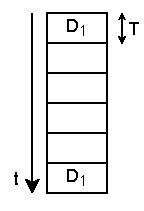
\includegraphics[width=0.3\textwidth]{strongly-regular-data}
		\caption[Strongly regular data stream]{Strongly regular data stream; the data quantity is constant in all packets.}
		\label{fig:strongly-regular-data-stream}
	\end{figure}

\subsubsection{Weakly Regular Data Stream}
\begin{itemize}
	\item If the quantity of data varies periodically (over time), then this is a \textit{weakly regular data stream}. 
	\item Example: Compressed video stream which uses a compression method such as \gls{mpeg}.
\end{itemize}


Figure {\ref{fig:weakly-regular-data-stream}} shows an example of weakly regular data stream.
	
%@@@@@@@@@@@@@@@@@@@@@@@@@@@@@@@@@@@@
%									@
%			FIGURE					@
%									@
%@@@@@@@@@@@@@@@@@@@@@@@@@@@@@@@@@@@@
	\begin{figure}[ht]
		\centering
		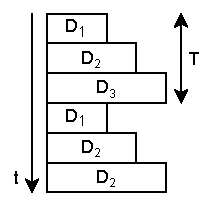
\includegraphics[width=0.3\textwidth]{weakly-regular-data}
		\caption[Weakly regular data stream]{Weakly regular data stream; the packets’ data stream varies periodically.}\label{fig:weakly-regular-data-stream}
	\end{figure}
	
\subsubsection{Irregular Data Stream}
Data streams are called irregular when the data quantity is neither constant, nor
changing by a periodic function (see Figure {\ref{fig:irregular-data-stream}}). This data stream is more difficult to transmit and process compared to the variants described earlier.

%@@@@@@@@@@@@@@@@@@@@@@@@@@@@@@@@@@@@
%									@
%			FIGURE					@
%									@
%@@@@@@@@@@@@@@@@@@@@@@@@@@@@@@@@@@@@
\begin{figure}[hb]
	\centering
	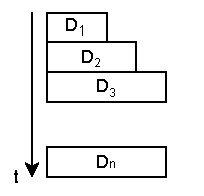
\includegraphics[width=0.3\textwidth]{irregular-data-stream}
	\caption[Irregular data stream]{Irregular data stream; the packets’ data quantity is not constant and does not vary periodically.}\label{fig:irregular-data-stream}
\end{figure}


When applying a compression method that creates a data stream with a variable
bit rate, the size of the single information units (each derived from a single image) is determined from the image content that has changed in respect to the previous image.
The size of the resulting information units normally depends on the video sequence and
the data stream is irregular.

\subsection{Contiguous Packets}
The third qualification characteristic concerns the continuity or the relationship
between consecutive packets. Are packets transmitted progressively, or is there a gap
between packets?  This can be seen as utilization of a certain system resource, such as a network.

\subsubsection{Interrelated/Continuous Data Stream}
\begin{itemize}
	\item All packets are transmitted one after the other without gaps in between.
	\item Additional information to identify user data is included, e.\ g.\, error detection codes.
	\item In this case specific resource is utilized at 100\%.
	\item Allows maximum throughput and achieves optimum utilization of a resource.
\end{itemize}
Figure {\ref{fig:interrelated-data-stream}} shows an interrelated/continuous information transfer.

%@@@@@@@@@@@@@@@@@@@@@@@@@@@@@@@@@@@@
%									@
%			FIGURE					@
%									@
%@@@@@@@@@@@@@@@@@@@@@@@@@@@@@@@@@@@@
\begin{figure}[hb]
	\centering
	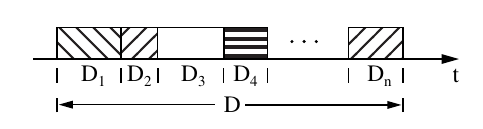
\includegraphics[width=0.8\textwidth]{interrelated-data-stream}
	\caption[Interrelated data stream.]{Interrelated data stream; packets are transmitted without gaps in between.}\label{fig:interrelated-data-stream}
\end{figure}

\subsubsection{Non-interrelated/Discrete Data Stream}
\begin{itemize}
	\item The transmission of an interrelated data stream over a higher-capacity channel
	causes gaps between packets.
	\item Each data stream that includes gaps between its information units is called a \textit{non-interrelated/discrete} data stream.
	\item It is not important if gaps exist among all packets or if the duration of gaps varies.
\end{itemize}
 Figure {\ref{fig:noninterrelated-data-stream}} shows an example of non-interrelated data stream.
 
%@@@@@@@@@@@@@@@@@@@@@@@@@@@@@@@@@@@@
%									@
%			FIGURE					@
%									@
%@@@@@@@@@@@@@@@@@@@@@@@@@@@@@@@@@@@@
\begin{figure}[ht!]
	\centering
	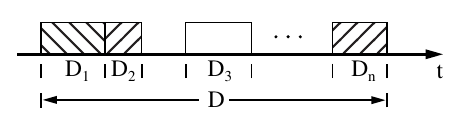
\includegraphics[width=0.8\textwidth]{non-interrelated-data-stream}
	\caption[Non-interrelated data stream.]{Non-interrelated data stream; there are gaps between packets.}\label{fig:noninterrelated-data-stream}
\end{figure}


\section{Information Units}
Continuous (time-dependent) media consist of a (temporal) sequence of information units. Such an information unit is called a \gls{ldu}, which is based on \gls{pdu}. An \gls{ldu}’s information quantity and data quantities can have different meanings:

%@@@@@@@@@@@@@@@@@@@@@@@@@@@@@@@@@@@@
%									@
%			FIGURE					@
%									@
%@@@@@@@@@@@@@@@@@@@@@@@@@@@@@@@@@@@@
\begin{figure}[hb!]                                                                    
	\centering
	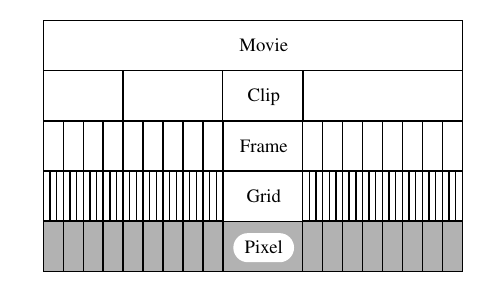
\includegraphics[width=\textwidth]{information-units}
	\caption[Information units.]{Granularity of a motion video sequence showing its \gls{ldu}s}\label{fig:information-units}
\end{figure}

\begin{itemize}
	\item In Figure {\ref{fig:information-units}}, we see that the uncompressed video sequence consists of single \textit{clips}, each representing a \textit{scene}.
	\item Each of these scenes consists of a sequence of single \textit{images}.
	\item An image can be divided, for example \(16\times16\) groups of \textit{pixels}.
	\item In turn, each pixel contains a \textit{luminance} value and a \textit{chrominance} value.
\end{itemize}

This means that a single image is not the only possible LDU in a motion video sequence. A scene or a pixel can also be an \gls{ldu}. The redundancies in single image sequences of an \gls{mpeg}-encoded video stream can be used to reduce the data quantity by applying an interframe compression method. In this case, the
smallest self-sufficient meaningful units are single-image sequences.



A phenomenon called granularity characterizes the hierarchical decomposition of
an audio or video stream in its components. This example uses a motion video to generally describe extensive information units. 

We distinguish between closed and open \gls{ldu}s:
\begin{itemize}
	\item \textit{Closed \gls{ldu}s} have a well-defined duration. They are normally stored sequences. Example: data stream of audio samples in the computer.
		
	\item In \textit{Open \gls{ldu}s}, the data stream’s duration is not known in advance. Such a data stream is delivered to the computer by a camera, a microphone, or a similar device.
\end{itemize}


\newpage\thispagestyle{empty}
 % Chapter-1: Multimedia System
\chapter{Sound and Audio}

Sound is a physical phenomenon caused by vibration of material, such as a sarangi string (\textnp{\footnotesize{सारङ्गीकाे तार}}) or a madal (\textnp{\footnotesize{मादल}}). This type of vibration triggers pressure wave fluctuations in the air around the material. The pressure waves propagate through the air in a wave-like motion. When a wave reaches the human ear, We hear a sound.




\section{Sound, Representation and Formats}
\subsection{Basic Sound Concept}
Sound is produced by the vibration of matter. During the vibration, pressure variations are created in the air surrounding it. The pattern of this oscillation (see Figure \ref{fig:oscillation}) is called \textit{waveform}. 


%@@@@@@@@@@@@@@@@@@@@@@@@@@@@@@@@@@@@
%									@
%			FIGURE					@
%									@
%@@@@@@@@@@@@@@@@@@@@@@@@@@@@@@@@@@@@

\begin{figure}[ht!]
	\centering
	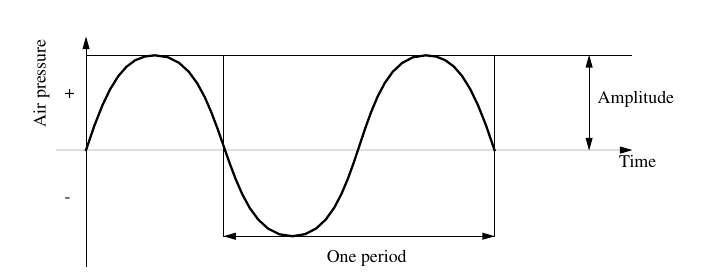
\includegraphics[width=\textwidth]{pressure-wave-osc}
	\caption{Pressure wave oscillation in the air.}{\label{fig:oscillation}}
\end{figure}


This wave form occurs repeatedly at regular \textit{intervals} or \textit{periods}. Sound waves have a natural origin, so they are never absolutely uniform or periodic. 
\begin{itemize}
	\item A sound that has a recognizable periodicity is referred to as \textit{music}.
	\item Examples of \textit{periodic} sound: sounds generated by musical
	instruments, vocal sounds, wind sounds, or a bird’s twitter.
	\item Examples of \textit{non-periodic} sounds: drums, coughing, sneezing, etc.
\end{itemize}

\subsubsection{Frequency}
A sound's frequency is the \textit{reciprocal value of its period}. The frequency represents the number of periods per second and is measured in \gls{hz} or \gls{cps}.

A common abbreviation is \gls{khz}, which describes 1,000 oscillations per second, corresponding to 1,000Hz. Sound processes that occur in liquids, gases, and solids are classified by frequency range:

\begin{multicols}{2}
\begin{itemize}
	\item Infrasonic: 0 to 20\gls{hz}
	\item Audiosonic: 20\gls{hz} to 20\gls{khz}
	\item Ultrasonic: 20\gls{khz} to 1GHz
	\item Hypersonic: 1GHz to 10THz
\end{itemize}
\end{multicols}


 Multimedia systems make use of sound only within frequency range of human hearing. Sound within human hearing range is called \textit{audio}. The waves in the audiosonic frequency range are called \textit{acoustic signals}. 

\begin{itemize}
	\item Speech is an acoustic signal produced by humans.
	\item Music signals have a frequency range between 20\gls{hz} and 20\gls{khz}.
	\item Beside speech and music, we denote any other audio signal as \textit{noise}.
\end{itemize}


\subsubsection{Amplitude}
A sound has a property called \textit{amplitude}, which humans perceive subjectively as
loudness or volume. The amplitude of a sound is a measuring unit used to deviate the
pressure wave from its mean value (idle state).

\subsection[Representation]{Sound Representation}
The smooth, continuous curve of a sound waveform is not directly represented in
a computer. A computer measures amplitude of the waveform at regular time
intervals to produce a series of numbers. Each of these measurements is a \textit{sample}. Figure {\ref{fig:wave-sampling}} shows one period of a digitally sampled wave.

%@@@@@@@@@@@@@@@@@@@@@@@@@@@@@@@@@@@@
%									@
%			FIGURE					@
%									@
%@@@@@@@@@@@@@@@@@@@@@@@@@@@@@@@@@@@@

\begin{figure}[H]
	\centering
		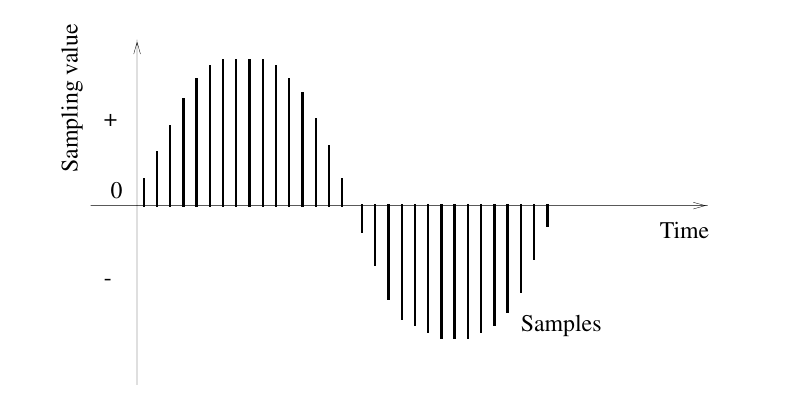
\includegraphics[width=0.8\textwidth]{sampling-a-wave}
	\caption{Sampling a wave.}{\label{fig:wave-sampling}}
\end{figure}


The mechanism that converts an audio signal into a sequence of digital samples is called an \gls{adc} and a \gls{dac} is used to achieve the opposite conversion.

\subsection{Sampling Rate}
The rate at which a continuous wave form is sampled (see Figure {\ref{fig:wave-sampling}}) is called the \textit{sampling rate}. It is measured in \gls{hz}. 

For example, CDs are sampled at a rate of \(44,100\)\gls{hz}, which may appear to be above the frequency range perceived by humans. However, the bandwidth in this case, \(20,000Hz-20Hz = 19,980Hz\) that can represent a digitally sampled audio signal is only about half as big as a CD's sampling rate, because CDs use the \textbf{Nyquist sampling theorem}\footnote{Nyquist’s Sampling Theorem: The Sampling frequency for a signal must be at least twice
	the highest frequency component in the signal}. This means
that a sampling rate of $ 44,100Hz $ covers only frequencies in the range from $ 0Hz $ to
$ 22,050Hz $. This limit is very close to the human hearing capability.


\subsection{Quantization}
The digitization process requires two steps. 
\begin{itemize}
	\item First the analog signal must be sampled. This means that only a discrete set of values is retained at (generally regular) time
	or space intervals. 
	
	\item The second step involves quantization. The \textit{quantization} process consists of converting a sampled signal into a signal that can take only a limited number of values.
\end{itemize}
 
An 8-bit quantization provides 256 possible values, while a 16-bit quantization in \gls{cd} quality results in more than $ 65,536 $ possible values. Figure \ref{fig:3bit-quantization} shows a 3-bit quantization.

%%%%%%%%%%%%%%%%%%%%%%%%%%%%%%%%%%%%%%%%%
%										%
%				FIGURE				   	%
%										%
%%%%%%%%%%%%%%%%%%%%%%%%%%%%%%%%%%%%%%%%%
\begin{figure}[H]
	\centering
		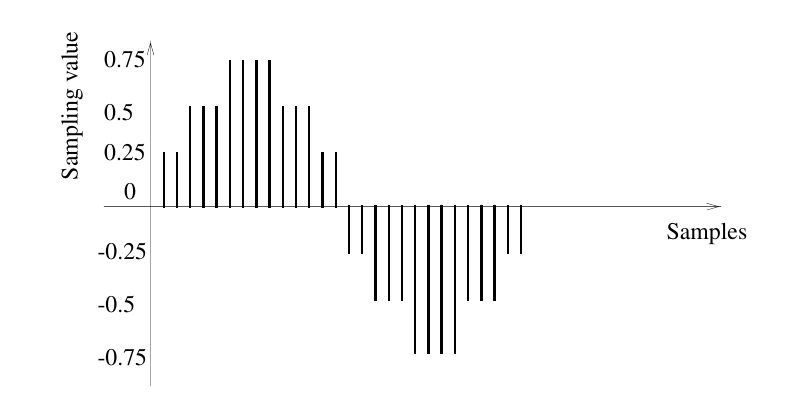
\includegraphics[width=\textwidth]{3-bit-quantization}
	\caption{3-bit quantization.}{\label{fig:3bit-quantization}}
\end{figure}

%-------------------FIGURE END---------------------------

The values transformed by a 3-bit quantization process can accept eight different
characteristics: \(0.75, 0.5, 0.25, -0.25, -0.5, -0.75, and\, -1\), so that we obtain an
“angular-shape” wave. This means that the lower the quantization (in bits), the more the
resulting sound quality deteriorates.

\subsection{Sound Hardware}
Before sound can be processed, a computer needs input/output devices. Microphone
jacks and built-in speakers are devices connected to an \gls{adc} and \gls{dac}, respectively for the input and output of audio.

\subsection{Formats}
\begin{itemize}
	\item Popular audio file formats include:
		\begin{itemize}
			\item \texttt{.au}(Origin: Unix, Sun),
			\item \texttt{.aiff}(Mac),
			\item \texttt{.wav} (PC)
		\end{itemize}
	\item Compression can be utilized in some of the above but is not Mandatory.
	\item A simple and widely used (by above) audio compression method is \gls{adpcm}.
			\begin{itemize}
				\item Based on past samples, it predicts the next sample and
				encodes the difference between the actual value and the
				predicted value.
			\end{itemize}
		\item Many formats linked to audio applications.
		\item Most audio formats use compression.
\end{itemize}

Audio format defines the quality and loss of audio data. Based on application different type of audio format are used. Audio formats are broadly divided into three parts:

\begin{enumerate}
	\item \textit{Uncompressed Format}. Example: \gls{wav}, \gls{aiff}, AU.
	\item \textit{Lossy Compressed format}. Example: \gls{mp3}, \gls{aac}, \gls{wma} Lossy.
	\item \textit{Lossless Compressed Format}. Example: \gls{flac}, \gls{alac}.
\end{enumerate}

 
\section[Basic Music (MIDI)]{Basic Music (MIDI)}
Music can be described in a symbolic way. On paper, we have the full scores.
Computers and electronic musical instruments use a similar technique, and most of
them employ the Musical Instrument Digital Interface (MIDI), a standard developed in
the early 1980s. The \gls{midi} standard defines how to code all the elements of musical
scores, such as sequences of notes, timing conditions, and the instrument to play each
note.

The \gls{midi} interface between electronic musical instruments and computers is a small piece of equipment that plugs directly into the computer's serial port and allows transmission of music signals. 

\subsection[Concepts]{MIDI Concepts}
MIDI represents a set of specifications used in instrument development so that
instruments from different manufacturers can easily exchange musical information. A MIDI interface is composed of two different components:

\begin{itemize}
	\item \textbf{Hardware} to connect the equipment. \gls{midi} hardware specifies the physical connection of musical instruments. It adds a \gls{midi} port to an instrument, it specifies a \gls{midi} cable (that connects two instruments), and processes electrical signals received over the cable.
	
	\item \textbf{A data format} that encodes information to be processed by the hardware. The MIDI data format does not include the encoding of individual sampling values, such as audio data formats. Instead, \gls{midi} uses a specific data format for each instrument, describing things like the start and end of scores, the basis frequency, and loudness, in addition to the instrument itself.
	
\end{itemize}
The MIDI data format is digital and data are grouped into \gls{midi} messages. When
a musician plays a key, the \gls{midi} interface generates a \gls{midi} message that defines the start of each score and its intensity. This message is transmitted to machines connected to the system. As soon as the musician releases the key, another signal (\gls{midi} message) is created and transmitted.

\subsection[Components]{Components of a MIDI System}

\subsubsection*{Synthesizer}
	\begin{itemize}
	\item It is a sound generator (various pitch, loudness, tone colour).
	\item A good (musician's) synthesizer often has a microprocessor, keyboard, control panels, memory, etc. 
\end{itemize}

\subsubsection*{Sequencer}
	\begin{itemize}
		\item It can be a standalone unit or a software program for a personal computer.
		\item It has one or more MIDI INs and MIDI OUTs. 
	\end{itemize}

\subsubsection*{Track}	
	\begin{itemize}
		\item Track in sequencer is used to organize the recordings.
		\item Tracks can be turned on or off on recording or playing back. 
	\end{itemize}
	
\subsubsection*{Channel}
	\begin{itemize}
		\item MIDI channels are used to separate information in a MIDI system.
		\item There are 16 MIDI channels in one cable.
		\item Channel numbers are coded into each MIDI message. 
	\end{itemize}
	
\subsubsection*{Timbre}
	\begin{itemize}
		\item The quality of the sound, e.g., flute sound, cello sound, etc.
		\item Multitimbral - capable of playing many different sounds at the same time (e.\ g.\ , piano, brass, drums, etc).
	\end{itemize}
	
\subsubsection*{Pitch}
	\begin{itemize}
		\item Musical note that the instrument plays. 
	\end{itemize}
		
\subsubsection*{Voice}
	\begin{itemize}
		\item Voice is the portion of the synthesizer that produces sound.
		\item Synthesizers can have many (12, 20, 24, 36, etc.) voices.
		\item Each voice works independently and simultaneously to produce sounds of different timbre and pitch.
	\end{itemize}
		
\subsubsection*{Patch}
	\begin{itemize}
		\item The control settings that define a particular Timbre.
	\end{itemize}



\subsection[Devices]{MIDI Devices}
%Through the MIDI interface, a computer can control output of individual instruments. On the other hand, the computer can receive, store or process coded musical data through the same interface. The data are generated with a \textit{keyboard} and reproduced through a sound generator. A \textit{sequencer} can store data. Further, it may
%also modify the musical data. In a multimedia system, the sequencer is a computer
%application.

%An instrument that complies with both components defined by the MIDI standard
%is a MIDI device (e.g., a synthesizer) able to communicate with other MIDI devices
%over channels. The MIDI standard specifies 16 channels. A MIDI device is mapped
%onto a channel. Musical data transmitted over a channel are reproduced in the synthe-
%sizer at the receiver’s end. The MIDI standard identifies 128 instruments by means of numbers, including noise effects (e.g., a phone ringing or an airplane take-off). For
%example:
%\begin{itemize}
%	\item  $ 0 $ specifies a piano
%	\item $ 12 $ a marimba
%	\item $ 40 $ a violin, and 
%	\item $ 73 $ a flute
%\end{itemize}
%
%Some instruments enable a user to play one single score (e.g., a flute) exclusively,
%while other instruments allow concurrent playing of scores (e.g., an organ). The maximum number of scores that can be played concurrently is an important property of synthesizers. This number can vary between 3 and 16 scores per channel.

A computer uses the \gls{midi} interface to control instruments for playout. The computer can use the same interface to receive, store, and process encoded musical data. 

\begin{itemize}
	\item In the \gls{midi} environment, these data are generated on a \textit{keyboard} and played out by a \textit{synthesizer}.
	\item A typical synthesizer is similar to a regular piano keyboard.
	\item A \textit{sequencer} is used to buffer or modify these data. In a multimedia application, the sequencer is a computer application.
\end{itemize}

The heart of any \gls{midi} system is the \gls{midi} \textit{synthesizer} device. A typical synthesizer looks like a simple piano keyboard with a panel full of buttons. Most synthesizers have the following common components:

\subsubsection*{Sound Generator}
\begin{itemize}
	\item The principal purpose of the generator is to produce an audio signal that
	becomes sound when fed into a loudspeaker. 
	
	\item By varying the voltage oscillation of the audio signal, a sound generator changes the quality of the sound – its pitch, loudness and tone – to create wide variety of
	sounds and notes.
\end{itemize}

\subsubsection*{Microprocessor}
\begin{itemize}
	\item The microprocessor communicates with the keyboard to know what notes the musician is playing, and with the control panel to know what
	commands the musician wants to send to the microprocessor. 
	\item The microprocessor then specifies note and sound commands to the sound generators.
\end{itemize}


\subsubsection*{Keyboard}
\begin{itemize}
	\item The keyboard affords the musician's direct control of the synthesizer.
	\item Pressing keys on the keyboard signals the microprocessor knows what
	notes to play and how long to play them.
\end{itemize}


\subsubsection*{Control Panel}
\begin{itemize}
	\item The control panel controls those functions that are not directly
	concerned with notes and durations. 
	\item It includes: 
		\subitem a \textit{slider} that sets the overall volume of the synthesizer, 
		\subitem a \textit{button} that turns the synthesizer on and off, and 
	\subitem a \textit{menu} that calls up different patches for the sound
	generators to play.
\end{itemize}


\subsubsection*{Auxiliary Controller}
They are available to give more control over the notes played on the
keyboard.

\subsubsection*{Memory}
Synthesizer memory is used to store patches for the sound generators
and settings on the control panel.\\

\noindent There are many other \gls{midi} devices that augment the standard synthesizer in a \gls{midi} system. Examples are drum machines which specialize in percussion sound's and rhythms, the master keyboard which increases the quality of the synthesizer keyboard, guitar controllers, guitar synthesizers, drum pad controllers and so on.

\subsection[Messages]{MIDI Messages}
 \gls{midi} messages are used by \gls{midi} devices to communicate with each other.
 
% \subsubsection[Structure]{Structure of MIDI Messages} 
 \subsubsection*{Structure of MIDI Messages} 

 \begin{itemize}
 	\item \gls{midi} message includes a \textit{status byte} and up to two \textit{data bytes}.
 	\item \textit{Status byte}
 	\begin{itemize}
 		\item The most significant bit of status byte is set to 1.
 		\item The 4 low-order bits identify which channel it belongs to.
 		\item The 3 remaining bits identify the message.
 	\end{itemize}
 	\item The most significant bit of data byte is set to 0. 
 \end{itemize}

%\subsubsection[Classification]{Classification of MIDI Messages}
\subsubsection*{Classification of MIDI Messages}

%@@@@@@@@@@@@@@@@@@@@@@@@@@@@@@@@@@@@
%									@
%			FIGURE					@
%									@
%@@@@@@@@@@@@@@@@@@@@@@@@@@@@@@@@@@@@
\begin{figure}[ht!]
	\centering
	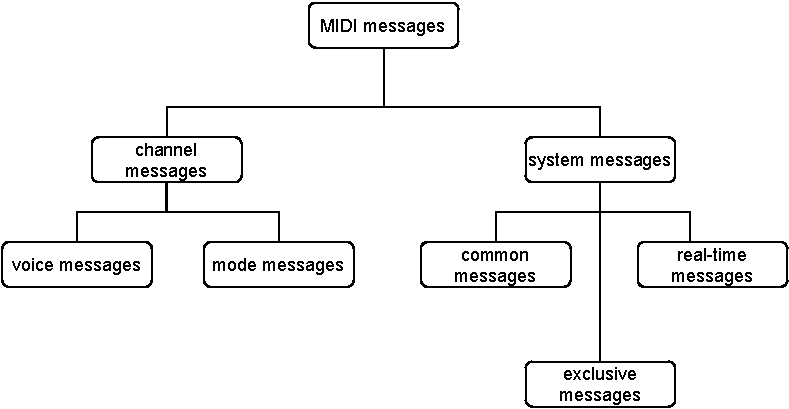
\includegraphics[width=0.9\textwidth]{midi-messages}
	\caption{Classification of \gls{midi} messages.}\label{fig:midi-messages}
\end{figure}

\begin{enumerate}[label=\Alph*)]
	\item \textbf{Channel messages}:  Messages that are transmitted on individual channels rather than globally to all devices in the \gls{midi} network.
	
		\begin{enumerate}[label=\alph*)]
			\item \textbf{Channel voice messages}
			
			    \begin{itemize}
			    	\item Instruct the receiving instrument to assign particular sounds to its voice.
			    	\item Turn notes on and off.
			    	\item Alter the sound of the currently active note or notes.
			    \end{itemize}
		    
		\item \textbf{Channel mode messages}
		
		\begin{itemize}
			\item Channel mode messages are a special case of the Control Change message. The difference between a Control message and a Channel Mode message is in the first data byte. 
			
			\item Channel mode messages determine how an instrument will process \gls{midi} voice messages. 
		\end{itemize}
		
		
		\end{enumerate}
	
	\item \textbf{System Messages}: System messages carry information that is not channel specific, such as timing signal for synchronization, positioning information in pre-recorded \gls{midi} sequences, and detailed setup information for the destination device.  
	  \begin{enumerate}
	  	\item \textbf{System real-time messages}: messages related to synchronization 
	  	\item \textbf{System common messages}: are commands that prepare sequencers and
	  	synthesizers to play a song. They are used for song selection, tuning the
	  	synthesizers etc.
	  	 \item \textbf{System exclusive message}: 
	  	 \begin{itemize}
	  	 	\item Messages related to things that cannot be standardized.
	  	 	\item Addition to the original \gls{midi} specification. 
	  	 	\item It is just a stream of bytes, all with their high bits set to 0, bracketed by a pair of system exclusive start and end messages.
	  	 \end{itemize}
	  \end{enumerate}
  
 
\end{enumerate}

\subsection[Standards]{MIDI Standards}
\begin{itemize}
	\item The \gls{midi} clock is used by a receiver to synchronize itself to the sender’s clock.
	\item To allow synchronization, 24 identifiers for each quarter note are transmitted. 
	\item Alternatively, the \gls{smpte} timing code
	can be sent to allow receiver-sender synchronization. 
	\item \gls{smpte} defines a frame format by
	\(hours:minutes:seconds:\), for example \(30\, frames/s\). This information is transmitted in a rate that would exceed the bandwidth of existing \gls{midi} connections.
	\item The \gls{midi} time code is normally used for synchronization because it does not transmit the entire time representation of each frame.
\end{itemize}


\subsection[Software]{MIDI Software}
Once a computer is connected to a \gls{midi} system, a variety of \gls{midi} applications can run on it. Digital computers afford the composer or sound designer unprecedented levels of control over the evolution and combination of sonic events.

The software applications generally fall into four major categories:

\subsubsection*{Music recording and performance applications}
This category of applications provide functions such as recording of \gls{midi} messages as they enter the computer from other \gls{midi} devices, and possibly editing and playing back the messages in performance.
			
 \subsubsection*{Musical notations and printing applications}
This category allows writing music using traditional musical notation. The user can then play back the music using a performance program or print the music on paper for live performance or publication.
			
\subsubsection*{Synthesizer patch editors and librarians}
These programs allow information storage of different synthesizer patches on the computer's memory and disk drives, and editing of patches on the computer.
			
\subsubsection*{Music education applications}
These software applications teach different aspects of music using the computer monitor, keyboard and other controllers of attached \gls{midi} instruments.		


\section{Speech}
\subsection{Concept}
Speech can be processed by humans or machines. The field of study of the handling of digitized speech is called digital speech processing.

Speech is based on spoken languages, which means that it has a semantic content. Human beings use their speech organs without the need to knowingly control the generation of sounds. Speech understanding means the efficient adaptation to speakers and their speaking habits. 

%Despite the large number of different dialects and emotional pronunciations, we can understand each other’s language. The
%brain is capable of achieving a very good separation between speech and interference,
%using the signals received by both ears. It is much more difficult for humans to filter signals received in one ear only. The brain corrects speech recognition errors because it
%understands the content, the grammar rules, and the phonetic and lexical word forms.

The human speech signal comprises a subjective lowest spectral component known as the \textit{pitch}, which is not proportional to frequency. The human ear is most sensitive in the range of $ 600 Hz $ to $ 6000 Hz $ Speech signals have two important characteristics that can be used by speech processing applications:

\begin{itemize}
	\item Voiced speech signals have an almost periodic	structure over a certain time interval, so that these signals remain \textit{quasi-stationary} for about $ 30ms $.
	
	\item The spectrum of some sounds have characteristic maxima that normally involve up to five frequencies. These frequency maxima, generated when speaking, are called \textit{formants}. By definition, a \textit{formant} is a characteristic component of the quality of an utterance.
\end{itemize}

%A machine can also support speech generation and recognition. With computers, one
%can synthetically generate speech, where the generated signals do not sound quite
%natural but can be easily understood. on the other hand, a
%voice can sound natura,l but may be very difrcult to understand. Speech recognition
%often uses matching rules or statistically based methods. Problems are caused when
%dialects, emotional pronunciation and environmental noises are part of the audio
%signal. There are, and will continue to be in the near future, considerable differences
%between the speech generation and recognition efficiencies/capabilities of the human
%brain and a high-performance computer.

\subsubsection*{Speech Synthesis}
Computers can translate an encoded description of a message into speech. This scheme is called \textit{speech synthesis}. A particular type of synthesis is text-to-speech conversion.

Speech recognition is normally achieved by drawing various comparisons. The problems in speech recognition affecting the recognition quality
include dialects, emotional pronunciations, and environmental noise. 

\subsection[Generation]{Speech Generation/Output}

A major challenge in speech output is how to generate these signals in real time for a speech output system to be able, for instance, to convert text to speech automatically. Some applications (e.\ g.\ , time announcements) handle this task with a limited vocabulary, but most use an extensive if not unlimited vocabulary.

The speech, a machine outputs has to be understandable and should sound natural. In fact, understandability is compulsory and naturalness a nice thing to have to increase user acceptance.

It is important to understand the most important technical terms used in relation to speech output, including:

\begin{itemize}
	\item Speech basic \textit{frequency} means the lowest periodic signal share in the speech
	signal. It occurs in voiced sounds.
	
	\item A \textit{phoneme} is a member of the set of the smallest units of speech that serve to distinguish one utterance from another in a language or dialect. It is the smallest
	meaningful linguistic unit but does not carry content.
	
	\item \textit{Allophones} specify variants of a phoneme as a function of its phonetic environment.
	
	\item A \textit{morpheme} is a meaningful linguistic unit whether in free-form or bound form that contains no smaller meaningful parts. For example, house is a morpheme, while housing is not.
	
	\item A \textit{voiced sound} is generated by oscillations of the vocal cords. The characters $ M $,
	$ W $, and $ L $ are examples. Voiced sounds depend strongly on the speaker.
	
	\item \textit{Unvoiced sounds} are generated with the vocal cords open, for example, $ F $ and $ S $.
	These sounds are relatively independent of the speaker.
\end{itemize}

\noindent Exactly, there are:

\begin{itemize}
	\item \textbf{Vowels}: a speech sound created by the relatively free passage of breath
	through the larynx and oral cavity, usually forming the most prominent
	and central sound of a syllable.
	\item \textbf{Consonants}:  a speech sound produced by a partial or complete
	obstruction of the air stream by any of the various constrictions of the
	speech organs.
\end{itemize}

\subsection[Analysis]{Speech Analysis/Input}
Speech analysis/input deals with various applications, as shown in Figure {\ref{fig:speech-input}}.

%@@@@@@@@@@@@@@@@@@@@@@@@@@@@@@@@@@@@
%									@
%			FIGURE					@
%									@
%@@@@@@@@@@@@@@@@@@@@@@@@@@@@@@@@@@@@
\begin{figure}[h]
	\centering
	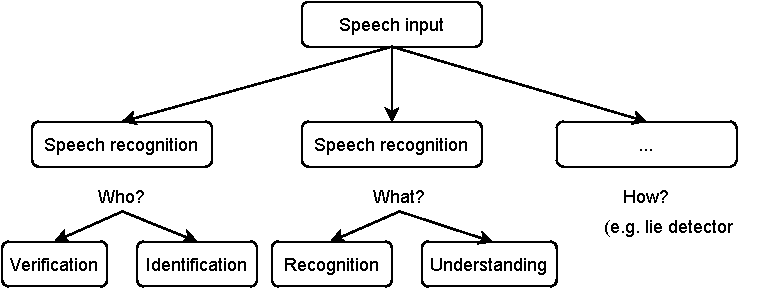
\includegraphics[width=0.8\textwidth]{speech-analysis}
	\caption{Speech input applications.}\label{fig:speech-input}
\end{figure}

In the speech input context, we need to ask three questions to obtain correct
answers: Who?, What?, and How?

\subsubsection*{Who?}
%Human speech has certain speaker-dependent characteristics, which means
%that speech input can serve to recognize a speaker. The computer is used to
%recognize an acoustic fingerprint of the speaker. 

Human speech has certain characteristics determined by a speaker. Hence,
speech analysis can serve to analyze \textit{who} is speaking, i.\ e.\ , to \textit{recognize a speaker} for his/her \textit{identification} and \textit{verification}. The computer identifies and verifies the speaker using an acoustic\footnote{An acoustic fingerprint is a digitally stored speech probe (e.\ g.\ , certain statement) of a person.} fingerprint.

\subsubsection*{What?}
%The central issue of speech input is to detect the speech contents themselves. A speech sequence is normally input to generate a piece of text. Typical applications are speech-controlled typewriters, language translation systems, or
%accessibility options for users with special needs.

Another main task of speech analysis is to analyze \textit{what has been said}, i.\ e.\ , to recognize and understand the speech signal itself. Based on speech sequence,
the corresponding text is generated.

\subsubsection*{How?}
Our third question relates to \textit{how a speech sample should be studied}. For example, a spoken sentence sounds differently if a person is angry or calm. One typical application is a lie detector.


\subsubsection{Speech Recognition}
In combination with speech synthesis, speech analysis enables us to implement media transformations.

The primary quality characteristic of each speech recognition session is determined by a probability of $ \leq 1 $ to recognize a word correctly. A word is always recognized only with a certain probability. Factors like environmental noise, room acoustics,
and the physical and psychical state of the speaker play an important role. 

For example, let's assume extremely bad individual word recognition with a probability of \(0.95\). This means that \(5\%\) of the words are incorrectly recognized. If we have a sentence with three words, the probability of recognizing the sentence correctly is
\(0.95 \times 0.95 \times 0.95 = 0.86\). 

This small example shows that a speech recognition system should have a very
high single-word recognition rate. Figure {\ref{fig:speech-recognition-principle}} shows the conceptual components of such a system.

%@@@@@@@@@@@@@@@@@@@@@@@@@@@@@@@@@@@@
%									@
%			FIGURE					@
%									@
%@@@@@@@@@@@@@@@@@@@@@@@@@@@@@@@@@@@@
\begin{figure}[hb!]
	\centering
	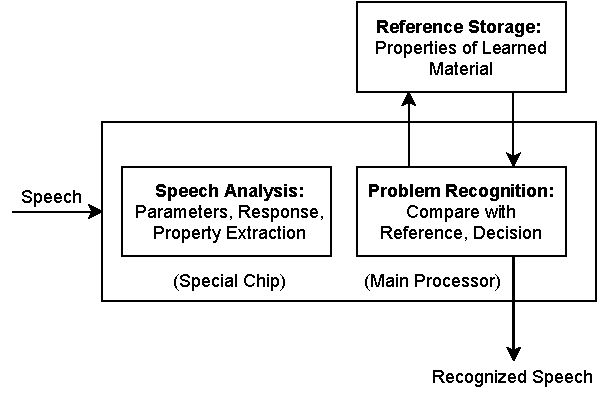
\includegraphics[width=0.8\textwidth]{speech-recognition-principle}
	\caption[The speech recognition principle]{The speech recognition principle: the tasks are distributed to system components by the basic principle ``extract characteristics to reduce data.''}\label{fig:speech-recognition-principle}
\end{figure}


The system is divided into system components according to a basic principle: ``Data Reduction Through Property Extraction''. 

 \textit{First}, speech analysis occurs where properties must be determined. Properties are extracted by comparison of individual speech element characteristics with a sequence of in advance given speech element characteristics. The characteristics are quantified where the concrete speech elements are present.


\textit{Second}, the speech elements are compared with existent references to determine the mapping to one of the existent speech elements. The identified speech can be stored,
transmitted or processed as a parameterized sequence of speech elements.

The principle shown in Figure {\ref{fig:speech-recognition-principle}} can be applied several times, each time referring to different characteristics. The application of the speech recognition principle can be divided into the steps shown in Figure {\ref{fig:speech-recognition-components}}.

%@@@@@@@@@@@@@@@@@@@@@@@@@@@@@@@@@@@@
%									@
%			FIGURE					@
%									@
%@@@@@@@@@@@@@@@@@@@@@@@@@@@@@@@@@@@@
\begin{figure}[ht!]
	\centering
		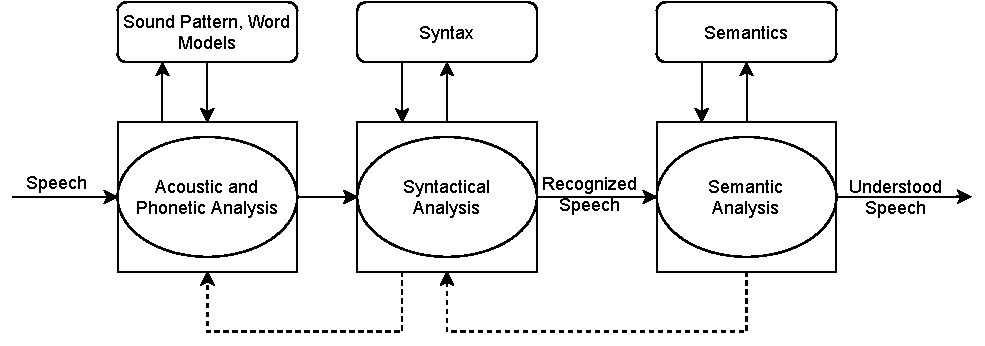
\includegraphics[width=\textwidth]{speech-recognition-components}
	\caption{Speech recognition components.}\label{fig:speech-recognition-components}
\end{figure}


The methods applied in the time and frequency ranges are:

\paragraph*{Acoustic and phonetic analysis}
In the first step, the principle is applied to a sound pattern and/or word model. An acoustical and phonetical \textit{analysis is performed}.

\paragraph*{Syntactic analysis}
The second step uses the speech units determined in the first step to run a syntactic analysis on them. This process can detect errors in the first run. It serves as an additional decision tool because the first step does not normally provide a final decision. The result is a \textit{recognized speech}.
	
\paragraph*{Semantic analysis}
The third step analyzes the semantics of the speech sequence recognized to this point. This step can detect errors from the previous decision process and remove them by using another interplay with other analytical methods. The implementation of this step is extremely difficult. The result of this step is an \textit{understood speech}.
	

\noindent These methods often work with characteristics in the time and/or frequency range. They are based on the same criteria and speech units (e.\ g.\ , formants or phonemes) as in speech output. 

\subsection[Transmission]{Speech Transmission}
Speech transmission is a field relating to highly efficient encoding of speech signals to enable low-rate data transmission, while minimizing noticeable quality losses. Some principles that are connected to speech generation and recognition are:

\subsubsection*{Pulse Code Modulation / Signal Form Coding}
Signal form encoding does not consider speech-dependent properties or parameters. Here, the goal is to achieve the most efficient coding of the audio signal. The data rate of a \gls{pcm}-coded stereo-audio signal with CD-quality requirements is:

\begin{align*}
rate & = 2 \times \frac{44,100}{s} \times \frac{16  {bits}}{8 bits/byte} \\
	& = 14,11,200 \times \frac{\cancel{bits}}{s} \times \frac{byte}{8\cancel{bits}}\\ 
	& = 14, 11, 200 \times \frac{byte}{8s}\\
	& = 1,76,400 \frac{byte}{s}\\
	& = 1,76,400 \times \frac{byte}{s} \times 8\: \textnormal{(\textnp{bits मा लैजान ८ ले गुणा गरेकाे})}  \\
	& = 14, 11, 200 bits/s\\
\end{align*}

%	\textnormal{\textnp{१}}
As a side note, telephone quality requires only $  64Kbit/s $ compared to $ 1,76,400byte/s $ for the case studied here. \gls{dpcm}
achieves $ 56Kbit/s $ in at least equal quality, while \gls{adpcm} enables a further reduction to $ 32Kbit/s $.

\subsubsection*{Source Encoding}
Parametric systems use source encoding. They utilize speech-specific characteristics to reduce data, for example the channel vocoder shown in Figure {\ref{fig:components-of-speech-transmission}}

%@@@@@@@@@@@@@@@@@@@@@@@@@@@@@@@@@@@@
%									@
%			FIGURE					@
%									@
%@@@@@@@@@@@@@@@@@@@@@@@@@@@@@@@@@@@@
\begin{figure}[ht!]
	\centering
		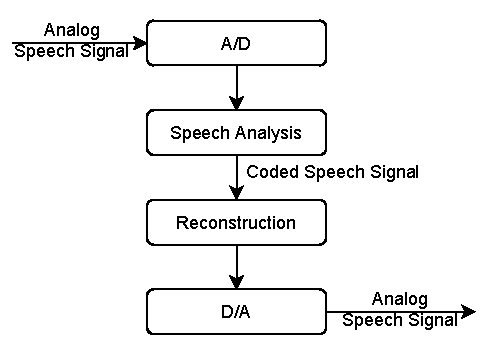
\includegraphics[width=0.6\textwidth]{components-of-speech-transmission}
	\caption[Components of a speech transmission system.]{Components of a speech transmission system using source encoding.}\label{fig:components-of-speech-transmission}
\end{figure}
%----------------------------figure end-----------------
A vocoder is an electronic mechanism that reduces speech signals to slowly varying signals that can be transmitted over communication systems of limited frequency bandwidth. A channel vocoder uses an enhanced subband encoding method.

In addition, the technique utilizes differences between \textit{voiced} and \textit{unvoiced} sounds. 
\begin{itemize}
	\item Unvoiced sounds are generated by means of a noise generator. 
	\item A pulse sequence is selected to generate voiced sounds.
\end{itemize}

\subsubsection*{Recognition/Synthesis Methods}

%Current research work attempts to further reduce the data volume by approximately $ 6Kbit/s $. The quality should always correspond to an uncompressed $ 64-Kbit/s $
%signal. Experts also study ways to reduce the transmission rate of speech signals by use
%of \textit{pure recognition-synthesis methods} (see Figure {\ref{fig:speech-recog-synthesis}}).

There have been attempts to reduce the transmission rate using pure recognition/synthesis methods. Speech analysis (recognition) follows on the sender side of a speech transmission system and speech synthesis (generation) follows on the receiver side (see Figure {\ref{fig:components-of-recognition-system}})

%@@@@@@@@@@@@@@@@@@@@@@@@@@@@@@@@@@@@
%									@
%			FIGURE					@
%									@
%@@@@@@@@@@@@@@@@@@@@@@@@@@@@@@@@@@@@
\begin{figure}[hb]
	\centering
		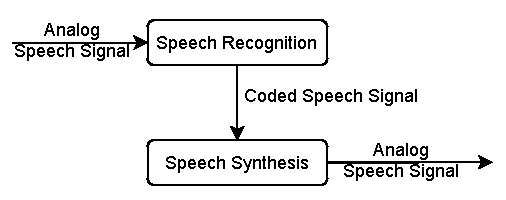
\includegraphics[width=0.8\textwidth]{components-of-recognition-system}
	\caption[Recognition/synthesis systems.]{Components of a recognition/synthesis system for speech transmission.}\label{fig:components-of-recognition-system}
\end{figure}


Only the speech element characteristics are transmitted, for example formants containing data about the center frequencies and bandwidths for use by digital filters.

\subsubsection*{Achievable Quality}
One of the most important aspects of speech and audio transmission in multimedia systems is the minimal achievable data rate in a defined quality. A data rate of less than $ 8Kbit/s $ for telephone quality can be achieved.

%@@@@@@@@@@@@@@@@@@@@@@@@@@@@@@@@@@@@
%									@
%			FIGURE					@
%									@
%@@@@@@@@@@@@@@@@@@@@@@@@@@@@@@@@@@@@
\begin{figure}[h]
	\centering
		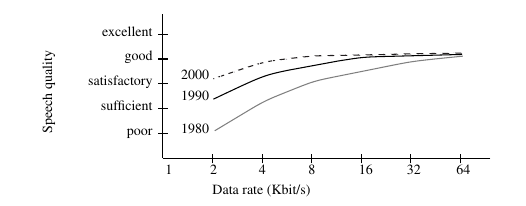
\includegraphics[width=\textwidth]{archievable-quality}
	\caption{Quality of compressed speech in relation to the compressed signal’s data rate.}\label{fig:archievable-quality}
\end{figure}


Figure \ref{fig:archievable-quality} relates the audio quality to the number of bits per sampling value. This ratio provides an excellent CD quality at a reduction of \(16 bits\) per sampling value to \(2 bits\) per sampling value, which means that only one eighth of the actual data rate is required to achieve this quality.
\newpage\thispagestyle{empty}
 % Chapter-2: Sound and Audio
\chapter{Image and Graphics}
An image is a spatial representation of an object, a two-dimensional or three-dimensional scene or another image. It can be real or virtual. An image may be abstractly thought of as a continuous function defining usually rectangular region of a plane.

A recorded image may be in a photographic, analog video signal or digital format. In computer vision, an image is usually a recorded image such as a-video-image, digital image or picture. In computer graphics, an image is always a digital image. In multimedia applications, all formats can be presented.

Graphics are normally created in a graphics application and internally represented as an assemblage of objects such as lines, curves, or circles. Attributes such as style, width, and color define the appearance of graphics. We say that the representation is aware of the semantic contents. The objects graphics are composed of can be individually deleted, added, moved, or modified later.⎄ In contrast, images can be from the real world or virtual and are not editable in the sense given above. They ignore the semantic contents. They are described as spatial arrays of values. 

The smallest addressable image element is called a \textit{pixel}. The array, and thus the set of pixels, is called a \textit{bitmap}. 

\subsubsection*{Drawback of Bitmaps}
The drawback of bitmaps is that they need much more storage capacity than graphics.

\subsubsection*{Advantage of Bitmaps}
Their advantage is that no processing is necessary before displaying them, unlike graphics where the abstract definition must be processed first to produce a bitmap.

\section{Basic Concepts, Digital Image Processing and Format and Graphics Format}

\subsection{Basic Concepts}
An image might be thought of as a function with resulting values of the light intensity at each point over a planar region. For digital computer operations, this function needs to be sampled at discrete intervals. The sampling quantizes the intensity values into discrete levels.

\subsection*{Digital Image Representation}
A digital image is represented by a matrix of numeric values each representing a quantized intensity value. When $ I $ is a two-dimensional matrix, then $ I(r, c) $ is the intensity value at the position corresponding to row $ r $ and column $ c $ of the matrix.

\begin{itemize}
	\item The points at which an image is sampled are known as \textit{picture elements}, commonly abbreviated as \textit{pixels}.
	\item The pixel values of intensity images are called \textit{gray scale levels}.
	\item The intensity at each pixel is represented by an integer and is determined from the continuous image by averaging over a small neighborhood around the pixel location.
	\item If there are just two intensity values, for example, black and white, they are represented by the numbers $ 0 $ and $ 1 $; such images are called \textit{binary-valued images}.
	\item When 8-bit integers are used to store each pixel value, the gray levels range from $ 0 $ (black) to $ 255 $ (white).
\end{itemize}
 
 \subsection{Digital Image Processing}
  Digital image processing is the use of a digital computer to process digital images through an algorithm. Digital image processing includes the following sub-areas:
  
  \begin{itemize}
  	\item \textit{Image analysis}: Is concerned with techniques for extracting descriptions from images that are necessary for higher level scene analysis methods.
  	\item \textit{Image recognition}: Is concerned with the techniques for recovering information about objects in the image.
  	\item \textit{Image enhancement}: Is concerned with the technique to improve the image and to correct some defects, such as:
  	\subitem colour and tonal adjustment
  	\subitem Transformation e.\ g.\ , scale, rotate
  	\subitem Special effects e.\ g.\ , texture, stylize, blur, sharpen 
  \end{itemize}
  
 \subsection{Image and Graphics Formats} 
  Most image formats incorporate some variation of a compression technique due to the large storage size of image files. Compression techniques can be classified into either \textit{lossless} or \textit{lossy}.
  
  A digital image consists of many picture elements, termed \textit{pixels}. The number of pixels that compose a monitor image determine the quality of the image (\textit{resolution}). Higher resolution always yields better quality.
  
  A bit-map representation stores the graphic/image data in the same manner that the computer monitor contents are stored in video memory.
  
  \subsubsection*{Monochrome/Bit-Map Images}
  \begin{itemize}
  	\item Each pixel is stored as a single bit (0 or 1)
  	\item Dithering is often used for displaying monochrome images
  \end{itemize}
  
  \subsubsection*{Gray-scale Images}
  Each pixel is usually stored as a byte (value between 0 to 255)
  
  \subsubsection*{8-bit Colour Images}
  \begin{itemize}
  	\item One byte for each pixel
  	\item Supports 256 out of the millions s possible, acceptable colour quality
  	\item Requires Colour Look-Up Tables (LUTs)\footnote{A color loop-up table (LUT) is a mechanism used to transform a range of input colors into another range of colors. }
  \end{itemize}
  
  \subsubsection*{24-bit Colour Images}
  \begin{itemize}
  	\item Each pixel is represented by three bytes (e.g., RGB)
  	\item Supports $ 256 \times 256 \times 256 $ possible combined colours ($ 1,67,77,216 $)
  	\item Most 24-bit images are 32-bit images, the extra byte of data for each pixel is used to store an alpha value representing special effect information
  \end{itemize}
  
  
 \subsubsection{Image Formats}
There are different kinds of image formats. Here we consider the image format that comes out of an image frame grabber, i.\ e.\ , the \textit{captured image format}, and the format when images are stored, i.\ e.\ , the \textit{stored image format}.

\paragraph*{Captured Image Format}
The format of an image is defined by two parameters:
\begin{itemize}
\item \textit{spatial resolution}, indicated in $ pixels \times  pixels $ and 
\item \textit{color encoding}, measured in \textit{bits per pixel}. 
\end{itemize}

The values of both parameters depend on the hardware and software used to input and output images.


%\subsubsection{Digital Image Processing}

\paragraph*{Stored Image Format}
To store an image, the image is represented in a \textit{two-dimensional matrix}, in which each value corresponds to the data associated with one image pixel. In bitmaps, these values are binary numbers. In color images, the values can be one of the following:

\begin{itemize}
	\item Three numbers that normally specify the intensity of the \textit{red}, \textit{green}, and \textit{blue}
	components.
	\item Three numbers representing references to a table that contains the red, green, and blue intensities.
	\item A single number that works as a reference to a table containing color triples.
	\item An index pointing to another set of data structures, which represents colors.
	\item Four or five spectral samples for each color.
\end{itemize}

When storing an image, information about each pixel, i.\ e.\ , the value of each color channel in each pixel, has to be stored. Additional information may be associated to the image as a whole, such as width and height, depth, or the name of the person who created the image. The necessity to store such image properties led to a number of flexible formats, such as RIFF (Resource Interchange File Format), or BRIM (derived from RIFF), which are often used in database systems. RIFF includes formats for bitmaps, vector drawings, animation, audio, and video. In BRIM, an image consists of width, height, authoring information, and a history field specifying the generation process or modifications.

The most popular image storing formats include: 
\begin{multicols}{2}
	\begin{itemize}
		\item PostScript, 
		\item GIF, 
		\item JPEG, 
		\item X11 BMP,
		\item TIFF, and 
		\item BMP.
	\end{itemize}
\end{multicols}


\paragraph*{PostScript}
PostScript is a fully fledged programming language optimized for printing graphics and text (whether on paper, film, or CRT). It was introduced by Adobe in 1985. The main purpose of PostScript was to provide a convenient language in which to describe images in a device-independent manner. This device independence means that the image is described without reference to any specific device features (e.\ g.\ , printer resolution) so that the same description could be used on any PostScript printer without modification.

\paragraph*{Graphics Interchange Format (GIF)}
The Graphics Interchange Format (GIF) was developed by CompuServe Information Service in 1987. Three variations of the GIF format are in use. The original specification, GIF87a, became a de facto standard because of its many advantages over other formats. GIF images are compressed to, 20 to 25 percent of their original size with no loss in image quality using a compression algorithm called \textit{LZW}.

\paragraph*{Tagged Image File Format (TIFF)}
The Tagged Image File Format (TIFF) was designed by Aldus Corporation and Microsoft in 1987 to allow portability and hardware independence for image encoding. It has become a de facto standard format. It can save images in an almost infinite number of variations. TIFF documents consist of two components:

\begin{itemize}
	\item The baseline part describes the properties that should support display programs. 
	\item The second part are extensions used to define properties, that is, the use of the CMYK color model to represent print colors.
\end{itemize} 

\subsubsection{Graphics Formats}
\paragraph*{X11 Bitmap (XBM) and X11 Pixmap (XPM)}
X11 Bitmap (XBM) and X11 Pixmap (XPM) are graphic formats frequently used in the UNIX world to store program icons or background images. These formats allow the definition of monochrome (XBM) or color (XPM) images inside a program code. The two formats use no compression for image storage.


\paragraph*{Bitmap (BMP)}
BMP files are device-independent bitmap files most frequently used in Windows systems. The BMP format is based on the RGB color model. BMP does not compress the original image. The BMP format defines a header and a data region. The header region (BITMAPINFO) contains information about size, color depth, color table, and compression method. The data region contains the value of each pixel in a line. 

Valid color depth values are 1, 4, 8, and 24. The BMP format uses the run-length encoding algorithm to compress images.

\section{Image Processing Fundamentals, Synthesis, Analysis, and Transformation}
Computer graphics deal with the graphical synthesis of real or imaginary images from computer-based models. In contrast to this technique, image processing involves
the opposite process, that is, the analysis of scenes, or the reconstruction of models from images representing 2D or 3D objects. The following sections describe some image analysis (image recognition) and image synthesis (image generation) basics.

\subsection{Image Analysis}
Image analysis involves techniques to extract descriptions from images, which are required by methods used to analyze scenes on a higher level. Techniques applied to analyzing images include:
\begin{itemize}
	\item the calculation of perceived colors and brightness, 
	\item a partial or full reconstruction of three-dimensional data in a scene, and 
	\item the characterization of the properties of uniform image regions.
	
\end{itemize}


Some image processing fields include:
\begin{multicols}{2}
	\begin{itemize}
		\item image improvement, 
		\item pattern discovery and recognition, 
		\item scene analysis, and 
		\item computer vision.
	\end{itemize}
\end{multicols}
 

Image improvement is a technique to improve the image quality by eliminating noise (due to external effects or missing pixels), or by increasing the contrast.

Pattern discovery and pattern recognition involve the discovery and classification of standard patterns and the identification of deviations from these patterns. An important example is OCR (Optical Character Recognition) technology, which allows efficient reading of print media, typed pages, or handwritten pages into a computer. 

Scene analysis and computer vision concern the recognition and reconstruction of 3D models of a scene consisting of various 2D images. A practical example is an industrial robot that measures the relative sizes, shapes, positions, and colors of objects.

\subsubsection{Image Recognition}
The complete process of recognizing objects in an image implies that we recognize a match between the sensorial projection (e.\ g.\ , by a camera) and the observed image. How an object appears in an image depends on the spatial configuration of the pixel values. The following conditions have to be met for the observed spatial configuration and the expected projection to match:

\begin{itemize}
	\item The position and the orientation of an object can be explicitly or implicitly derived from the spatial configuration.
	\item There is a way to verify that the derivation is correct.
\end{itemize}

Image recognition involves a number of different steps to successively transform object data into recognition information. A recognition method should include the following six steps:

\begin{multicols}{3}
\begin{enumerate}
	\item image formatting
	\item conditioning
	\item marking
	\item grouping
	\item extraction and 
	\item matching
\end{enumerate} 
\end{multicols}

These steps are shown schematically in Figure {\ref{fig:image-recognition-steps}}.

%%%%%%%%%%%%%%%%%%%%%%%%%%%%%%%%%%%%%%%%%
%										%
%				FIGURE				   	%
%										%
%%%%%%%%%%%%%%%%%%%%%%%%%%%%%%%%%%%%%%%%%
\begin{figure}[h]
	\centering
	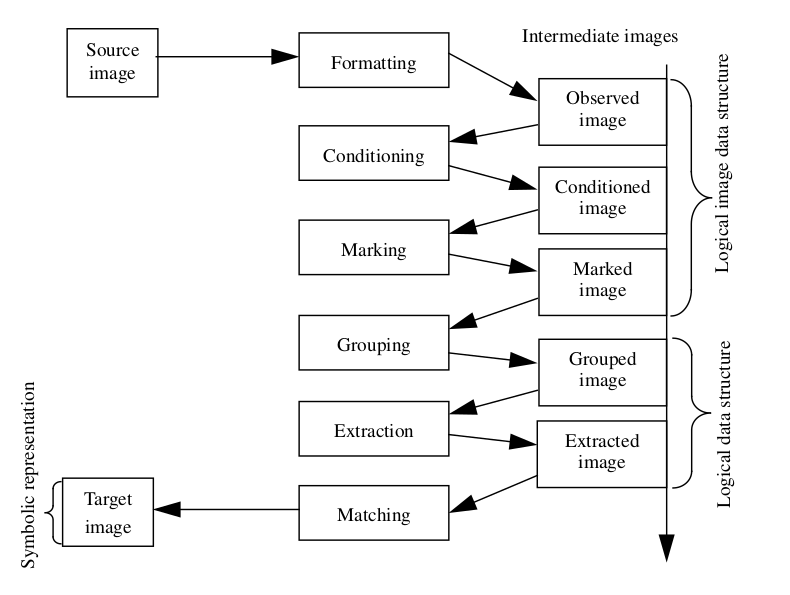
\includegraphics[width=0.8\textwidth]{image-recognition-steps}
	\caption{Steps involved in image recognition.}{\label{fig:image-recognition-steps}}
\end{figure}
%-------------------FIGURE END---------------------------

\paragraph*{The Image-Recognition Procedure/Steps}

The formatting step shoots an image by use of a camera and transforms the image into digital form (i.\ e.\ , pixels). The conditioning, marking, grouping,
extraction, and matching steps form a canonical division of the image recognition problem, where each step prepares and transforms the data required for the next step.
Depending on the application, it may be necessary to apply this sequence to more than one level of recognition and description. These five steps are:

\begin{steps}
\item \textit{Formatting}: The formatting step shoots an image by use of a camera and transforms the image into digital form (i.\ e.\ , pixels).
\item \textit{Conditioning}: 
		\begin{itemize}
			\item Conditioning is based on a model that assumes an image that can be observed is composed of information patterns, which are disturbed by irrelevant variations. \item Conditioning estimates the information pattern based on the observed image, so that noise can be suppressed. 
			\item Also, conditioning can normalize the background by ignoring irrelevant systematic or patterned variations. 
		\end{itemize}
		
\item \textit{Marking/Labeling}: 
		\begin{itemize}
			\item Marking is based on a model that assumes that information patterns have a structure in the form of spatial object arrangements, where each object is a set of interconnected pixels. 
			\item Marking determines to which spatial objects each pixel belongs.
		\end{itemize}
\item \textit{Grouping}: 
		\begin{itemize}
			\item The grouping operation identifies objects marked in the previous step by grouping pixels that are part of the same object.
			\item The grouping step includes the edge connection step. 
			\item A grouping operation that groups edges into lines is also called \textit{line fitting}.
			\item The grouping operation changes the logical data structure. 
			\item The original images, the conditioned, and marked images are all available as digital image data structures. 
		\end{itemize}
\item \textit{Extraction}: 	
			\begin{itemize}
				\item The grouping operation defines a new set of units, but they are incomplete because they have an identity but no semantic meaning. 
				\item The extraction operation calculates a list of properties for each pixel group. 
				\item Such properties can include center (gravity), surface, orientation, spatial moments, spatial grayscale moments, and circles.
			\end{itemize}
		
\item \textit{Matching}:
		\begin{itemize}
			\item When the extraction operation is finished, the objects occurring in an image are identified and measured, but they have no content meaning. 
			\item We obtain a content meaning by attempting an observation-specific organization in such a way that a unique set of spatial objects in the segmented image results in a unique image instance of a known object. 
			\item The matching operation determines how to interpret a set of related image objects, to which a given object of the three-dimensional world or a two-dimensional form is assigned.
			\item The classical method is template matching, which compares a pattern against stored models (templates) with known patterns and selects the best match.
		\end{itemize}
\end{steps}


\subsection{Image Synthesis}
Image synthesis is the process of creating new images from some form of image description. The kinds of images that are typically synthesized include:

\begin{itemize}
	\item \textit{Test Patterns}, Scenes with simple two-dimensional geometric shapes.
	\item \textit{Image Noise}, Images containing random pixel values, usually generated from specific parameterized distributions.
	\item \textit{Computer Graphics}, Scenes or images based on geometric shape descriptions. Often the models are three-dimensional, but may also be two-dimensional.
\end{itemize}
	Synthetic images are often used to verify the correctness of operators by applying them to known images. They are also often used for teaching purposes, as the operator output on such images is generally `clean', whereas noise and uncontrollable pixel distributions in real images make it harder to demonstrate unambiguous results. The images could be binary, gray level or color.

Image synthesis is an integral part of all computer-supported user interfaces and a necessary process to visualize 2D, 3D, or higher-dimensional objects. A large number
of disciplines, including education, science, medicine, construction, advertising, and the entertainment industry, rely heavily on graphical applications, for example:

\begin{itemize}
	\item \textbf{User interfaces}
	Applications based on the Microsoft Windows operating system have user interfaces to run several activities simultaneously and offer point-and-click options to select menu items, icons, and objects on the screen.
	
	\item \textbf{Office automation and electronic publishing}
	The use of graphics in the production and distribution of information has increased dramatically since desktop publishing was introduced on personal computers. Both office automation and electronic publishing applications can produce printed and electronic documents containing text, tables, graphs, and other types of drawn or scanned graphic elements. 
	
	\item \textbf{Simulation and animation for scientific visualization and entertainment}
	Animated movies and presentations of temporally varying behavior of real and simulated objects on computers have been used increasingly for scientific visualization. For example, they can be used to study mathematical models of phenomena, such as flow behavior of liquids, relativity theory, or nuclear and chemical reactions. Cartoon actors are increasingly modeled as three-dimensional computer-assisted descriptions. 
\end{itemize}

%Interactive computer graphics are the most important tool in the image production process since the invention of photography and television. With these tools, we cannot
%only create images of real-world objects, but also abstract, synthetic objects, such as images of mathematical four-dimensional surfaces.
%
%\subsubsection*{Dynamic Vs Static Graphics}
%The use of graphics is not limited to static images. Images can also vary dynamically. For example, a user can control an animation by adjusting the speed or changing
%the visible part of a scene or a detail. This means that dynamics are an integral part of
%(dynamic) graphics. Most modern interactive graphics technologies include hardware
%and software allowing users to control and adapt the dynamics of a presentation:
%
%\begin{itemize}
%	\item \textbf{Movement dynamics} 
%	
%	Movement dynamics means that objects can be moved or
%	activated relative to a static observer’s viewpoint. Objects may also be static while
%	their environment moves. A typical example is a flight simulator containing components that support a cockpit and an indicator panel. The computer controls the
%	movement of the platform, the orientation of the aircraft, and the simulated environment of both stationary and moving objects through which the pilot navigates.
%	
%	\item Adaptation dynamics: Adaptation dynamics means the current change of form,
%	color, or other properties of observed objects. For example, a system could represent the structural deformation of an aircraft in the air as a response to many different control mechanisms manipulated by the user. The more subtle and uniform
%	the change, the more realistic and meaningful is the result. Dynamic interactive
%	graphics offer a wide range of user-controllable modes. At the same time, these
%	modes encode and convey information, for example, 2D or 3D forms of objects in
%	an image, their gray levels or colors, and the temporal changes of their properties.
%\end{itemize}

\subsection{Image Transmission}
Image transmission takes into account transmission of digital images through computer networks. There are several requirements on the networks when images are transmitted:
\begin{itemize}
	\item The network must accommodate bursty data transport because image transmission is bursty (the burst is caused by the large size of the image).
	\item Image transmission requires reliable transport.
	\item Time-dependence is not a dominant characteristic of the image in contrast to audio/video transmission.
\end{itemize}

Image size depends on the image representation format used for transmission. There are several possibilities:

\subsubsection*{Raw image data transmission}
\begin{itemize}
	\item In this case, image is generated through a video digitizer and transmitted in its digital format. 
	\item The size can be computed in the following manner:
	\[
	Size = spatial\_resolution \times pixel\_resolution
	\]
	\item For example, the transmission of an image with a resolution of $ 640 \times 480 $ pixels and pixel quantization of 8 bits per pixel requires transmission of $ 3, 07,200 bytes $ through the network.
\end{itemize}

\subsubsection*{Compressed image data transmission}
\begin{itemize}
	\item In this case, the image is generated through a video digitizer and compressed before transmission. 
	\item Methods such as JPEG or MPEG are used to downsize the image. 
	\item The reduction of image size depends on the compression method and compression rate.
\end{itemize}

\subsubsection*{Symbolic image data transmission}
\begin{itemize}
	\item In this case, the image is represented through symbolic data representation as image primitives (e.g. 2D or 3D geometric representation), attributes and other control information. 
	\item This image method is used in computer graphics.
	\item Image size is equal to the structure size, which carries the transmitted symbolic information of the image.
\end{itemize}

\newpage\thispagestyle{empty} % Chapter-3: Image and Graphics
\chapter{Video and Animation}
Video data can be generated in two different ways: 

\begin{itemize}
	\item by recording the real world and 
	\item through synthesis based on a description
\end{itemize}

\section{Basic Video Concepts}
The human eye is the human receptor for taking in still pictures and motion pictures. Its inherent properties determine, in conjunction with neuronal processing, some of the basic requirements underlying video systems.

\subsection{Video Signal Representation}
In conventional black-and-white television sets, the video signal is usually generated by means of a Cathode Ray Tube (CRT). An electron beam carries corresponding pattern information, such as intensity in a viewed scene.

The representation of a video signal comprises three aspects: 
\begin{itemize}
	\item visual representation
	\item transmission, and 
	\item digitization.
\end{itemize}
\subsubsection{Visual Representation} 
A key goal is to present the observer with as realistic as possible a representation of a scene. In order to achieve this goal, the television picture has to accurately convey the spatial and temporal content of the scene. Important measures for this are:


\begin{enumerate}
	\item \textit{Vertical details and viewing distance}
	
	The geometry of a television image is based on the ratio of the picture width $ W $ to the picture height $ H $. This width-to-height ratio is also called the aspect ratio. The	conventional aspect ratio (for television) is $ 4/3=1.33 $. Figure {\ref{fig:decomposition-of-motion-picture}} shows an
	example of this ratio.

%%%%%%%%%%%%%%%%%%%%%%%%%%%%%%%%%%%%%%%%%
%										%
%				FIGURE				   	%
%										%
%%%%%%%%%%%%%%%%%%%%%%%%%%%%%%%%%%%%%%%%%
\begin{figure}[h]
	\centering
	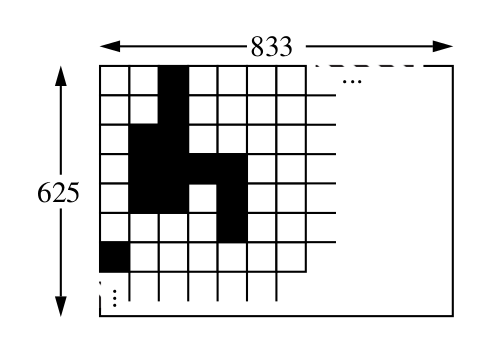
\includegraphics[width=0.8\textwidth]{decomposition-of-motion-picture}
	\caption{Decomposition of a motion picture.}{\label{fig:decomposition-of-motion-picture}}
\end{figure}
%--------------------------Figure end -------------------
The viewing distance $ D $ determines the angular field of view. This angle is usually calculated as the ratio of the viewing distance to the picture height ($ D/H $).

\item \textit{Horizontal detail and picture width}

The picture width normally used for television is $ (\frac{4}{3}  \times picture \:height )$ i.\ e.\ ($ 4/3 $ times the picture height). The horizontal field of view can be determined using the aspect ratio.

\item \textit{Total detail content of a picture}

The vertical resolution is equal to the number of picture elements of the picture height, while the number of horizontal picture elements is equal to the product of the vertical resolution and the aspect ratio. 

The product of the picture’s elements	vertically and horizontally is the total number of picture elements in the image. 

However, in the case of television pictures, not all lines (and columns) are visible to the observer. The invisible areas are often used to transmit additional information.

\item \textit{Depth perception}

In nature, humans perceive the third dimension, depth, by comparing the images perceived by each eye, which view from different angles. In a flat television picture, a considerable portion of depth perception is derived from the perspective appearance of the subject matter. 

Further, the choice of the focal length of the camera lens and changes in depth of focus influence depth perception.
	
\item \textit{Luminance and Chrominance}

Color perception is achieved by three signals, proportional to the relative intensities of \textit{red}, \textit{green}, and \textit{blue} light (RGB) present in each portion of the scene. These	are conveyed to the monitor separately and the tube reproduces them at each point in time (unlike a camera). Often a different signal division is used for transmission and storage: 
\begin{itemize}
	\item one brightness signal (luminance), and 
	\item two color difference signals (chrominance).
\end{itemize}


\item \textit{Temporal aspects of illumination}	 

This property is used in television, in films, and for video data in computer systems. The impression of motion is created by presenting a rapid succession of barely differing still pictures (frames). Between frames, the light is cut off briefly. 

Two conditions must be met in order to represent a visual reality through motion pictures.
\begin{itemize}
	\item First, the rate of repetition of the images must be high enough to ensure continuity of movements (smooth transition) from frame to frame. 
	\item Second, the rate must be high enough that the continuity of perception is not disrupted by the dark intervals between pictures.
\end{itemize}


\item \textit{Continuity of motion}

	It is known that continuous motion is only perceived as such if the frame rate is higher than 15 frames per second. To make motion appear smooth, at least 30 frames per second must be used if the scene is filmed by a camera and not generated synthetically.
		
\item \textit{Flicker}
	
	If the refresh rate is too low, a periodic fluctuation of the perceived brightness can result. This is called the flicker effect. The minimum refresh rate to avoid flicker is $ 50Hz $. Achieving continuous, flicker-free motion would thus require a high refresh rate. However, in both movies and television, there are technical measures	that allow lower refresh rates to be used.

\item \textit{Temporal aspect of video bandwidth}

	Temporal specification depends on the rate of the visual system to scan pixels, as well as on the human eye's scanning capabilities. From human visual perspective, the eye requires that a video frame be scanned every $ 1/25 $ second. This time is equivalent to the time during which a human eye does not see the flicker effect.
\end{enumerate}


\subsubsection{Transmission}
Video signals are often transmitted to the receiver over a single television channel. In order to encode color, consider the decomposition of a video signal into three subsignals. For reasons of transmission, a video signal is comprised of a luminance signal and two chrominance (color) signals. 


Several approaches to color encoding are described below.

\begin{itemize}
	\item \textit{RGB Signal}
	
	An RGB signal consists of separate signals for red, green, and blue. Every color can be encoded as a combination of these three primary colors. The values $ R $ (for red), $ G $ (for green), and $ B $ (for blue), are normalized such that white results when $ R+G+B = 1 $ in the normalized representation.
	
	\item \textit{YUV Signal}
	
	Since human vision is more sensitive to brightness than to color, a more suitable encoding separates the luminance from the chrominance (color information). Instead of separating colors, the brightness information (luminance $ Y $) is separated from the color information (two chrominance channels $ U $ and $ V $).⎄
	
	The YUV signal can be calculated as follows:
	\begin{align*}
	 	& Y = 0.30R + 0.59G + 0.11B  \\
	 	& U = (B-Y) \times 0.493  \\
		& V = (R-Y) \times 0.877&&
	\end{align*}

\item \textit{YIQ signal}

A similar encoding exists for NTSC’s YIQ signal:
	\begin{align*}
		& Y = 0.30R + 0.59G + 0.11B \\
		& I = 0.60R - 0.28G - 0.32B  \\
		& Q = 0.21R - 0.52G + 0.31B &&
	\end{align*}
\end{itemize}
\subsubsection*{Digitalization}
Before a motion picture can be processed by a computer or transmitted over a network, it must be converted from an analog to a digital representation.

This digitization process consists of the three steps of:
\begin{multicols}{3}
	\begin{enumerate}
		\item \textit{sampling},
		\item \textit{quantization}, and
		\item \textit{coding}.
	\end{enumerate}
\end{multicols}

In determining the sampling frequency, the \textbf{Nyquist Theorem} must be followed.
 
Nyquist theorem states that the signal being sampled cannot contain any frequency components that exceed half the sampling frequency. 

In order to prevent the base band from overlapping with repeating spectra and to allow for real hardware components not behaving ideally, the sampling rate is normally chosen somewhat higher than the limit dictated by the Nyquist Theorem.

Digitalization consists of sampling the gray (color) level in the picture at $ M \times N $ array of points. The next step in the creation of digital motion video is to digitize pictures in time and get a sequence of digital image per second for analog motion video.

Since the gray value of a sampled spot can take on any value in a continuous range, it must be quantized in order to be processed digitally. The gray-scale is subdivided into several ranges, and each pixel is assigned only one of these values.


\subsection{Computer Video Format}
The computer video format depends on the input and output devices for the motion video medium.

Current video digitalization hardware differs with respect to the resolution of the digital images (frames), quantization, and the frame rate (frames/second).

Motion video output depends on the display hardware used, usually a raster display. The typical architecture of such a device is shown in Figure {\ref{fig:raster-arch}}.


%%%%%%%%%%%%%%%%%%%%%%%%%%%%%%%%%%%%%%%%%
%										%
%				FIGURE				   	%
%										%
%%%%%%%%%%%%%%%%%%%%%%%%%%%%%%%%%%%%%%%%%
\begin{figure}[H]
	\centering
	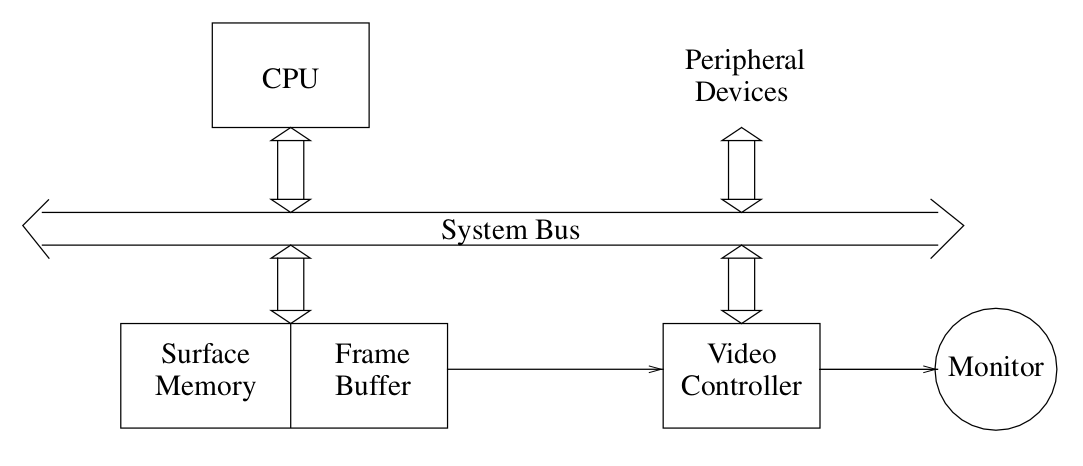
\includegraphics[width=0.8\textwidth]{raster-arch}
	\caption{Architecture of a raster display.}{\label{fig:raster-arch}}
\end{figure}
%--------------------------Figure end -------------------

\begin{itemize}
	\item The video controller displays the image stored in the frame buffer, accessing the buffer through a separate port as often as required by the video scanning rate. 
	\item The most important task is the constant refresh of the display. 
	\item Due to the disturbing flicker effect, the video controller cycles through the frame buffer, one scan line at a time, typically 60 times/second. 
	\item To display different colors on the screen, the system works with a Color Look-Up Table (CLUT or LUT). 
	\item At any given time, a limited number of colors ($ n $) are available for the whole picture. 
	\item The set of the $ n $ most frequently used colors is chosen from a color palette consisting of $ m $ colors, whereby in general  $n \ll m$.
\end{itemize}


Some computer video controller standards are given here as examples. Each of these systems supports different resolution and color presentation.

\begin{itemize}
	\item The \textit{Color Graphics Adapter (CGA)} has a resolution of $ 320 \times 200  $pixels with simultaneous presentation of four colors. Therefore, the storage capacity per image is:
	
	\begin{align*}
		320 \times 200 \: pixels \times \frac{2 \: bit/pixel}{8 \: bit/byte} = 16,000 \: bytes
	\end{align*}

\item The \textit{Enhanced Graphics Adapter (EGA)} supports display resolution of $ 640 \times 350 $ pixels with 16 simultaneous colors. The necessary storage capacity per frame is:

\begin{align*}
	640 \times 350 \: pixels \times \frac{4 \: bit/pixel}{8 \: bit/byte} = 1, 12,000 \: bytes
\end{align*}

\item The \textit{Video Graphics Array (VGA}) works mostly with a resolution of $ 640 \times 480 $ pixels with 256 simultaneous colors. The monitor is controlled via an analog RGB output. The necessary storage capacity per frame is:

\begin{align*}
	640 \times 480 \: pixels \times \frac{8 \: bit/pixel}{8 \: bit/byte} = 3, 07,200 \: bytes
\end{align*}

\item The \textit{Super Video Graphics Array (SVGA}) can present 256 colors at a resolution of $ 1,024 \times 768  $pixels. The necessary storage capacity per frame is:

\begin{align*}
	1,024 \times 768 \: pixels \times \frac{8 \: bit/pixel}{8 \: bit/byte} = 7,86,432 \: bytes
\end{align*}

Other SVGA modes include $ 1,280 \times 1,024 $ pixels and $ 1,600 \times 1,280 $ pixels.

\end{itemize}

\section{Animation}
To animate something is, literally, to bring it to life. An animation covers all changes that have a visual effect. Visual effects can be very different attributes: 

\begin{itemize}
	\item positions (\textit{motion dynamics}), form, color, transparency, structure, and 
	\item texture of an object (\textit{update dynamics}), as well as 
	\item changes in lighting, camera position, orientation, and focus.
\end{itemize}




Today, computer-based animations are produced, edited, and generated with the help of a computer using graphical tools to create visual effects. Naturally, the discipline of traditional, non-computer based animation continues to exist.

\subsection{Basic Concepts of Animation}

\subsubsection{Input Process}
\begin{itemize}
	\item Before the computer can be used, drawings must be digitized to create key frames.
	\item These digitized images can be produced by the computer using appropriate programs or created by digitizing photos or drawings. 
	\item The drawings may need to be carefully post-processed (e.\ g.\ , filtering) in order to clean up any glitches arising from	the input process.
\end{itemize}


\subsubsection{Composition Stage}
\begin{itemize}
	\item Individual frames in a completed animation are generated by using image composition techniques to combine foreground and background elements. 
\end{itemize}


\subsubsection{Inbetween Process}
\begin{itemize}
	\item The animation of movement from one position to another requires the composition of frames with intermediate positions (intermediate frames) between key frames.
	\item In computer-based animation, this in-between processing is done using interpolation methods. 
	\item In interpolation, the system obtains only the beginning and end positions. 
	\item Linear interpolation, sometimes called \textit{lerping}, is the simplest method.
	\item For example, if one uses lerping to calculate the intermediate positions of a ball that has been thrown in the air and uses only three key frames, as
	shown in Figure {\ref{fig:linear-interpolation}}(a), then the resulting motion of the ball, depicted in Figure {\ref{fig:linear-interpolation}}(b),
	is totally unrealistic.
\end{itemize}


%%%%%%%%%%%%%%%%%%%%%%%%%%%%%%%%%%%%%%%%%
%										%
%				FIGURE				   	%
%										%
%%%%%%%%%%%%%%%%%%%%%%%%%%%%%%%%%%%%%%%%%
\begin{figure}[H]
	\centering
	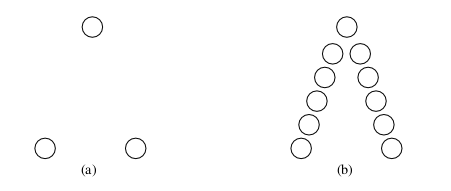
\includegraphics[width=0.8\textwidth]{linear-interpolation}
	\caption[Linear interpolation of the motion of a ball]{Linear interpolation of the motion of a ball: (a) key frames, (b) additional intermediate frames}{\label{fig:linear-interpolation}}
\end{figure}
%--------------------------Figure end -------------------

Due to the disadvantages of lerping, splines are often used to smooth out the interpolation between key frames. Splines can be used to smoothly vary different parameters as a function of time. With splines, individual points (or individual objects) can be moved in a natural fashion through space and time. 


\subsubsection{Changing Colors}
To process color changes, computer-based animation uses the Color Look-Up	Table (CLUT) or Look-Up Table (LUT). 
\begin{itemize}
	\item The animation is generated by manipulating the LUT.
	\item The simplest method is to cyclically change the colors of the LUT, thereby changing the colors of different parts of an image. 
	\item Performing LUT animation is relatively fast.
\end{itemize}

\subsection{Animation Languages}
Various languages exist to describe animations and new formal specification are currently being researched and further developed.

These specifications can be divided into the following three categories:

\subsubsection{Linear-List Notations}
In linear list notation each event in an animation is described by:
\begin{itemize}
	\item a beginning frame number, 
	\item an end frame number, and 
	\item an action (event) that is to be performed.
\end{itemize}

 Actions typically accept input parameters in the form of an instruction such as the following:
\begin{lstlisting}[numbers=none]
42, 53, B, ROTATE "PALM", 1, 30
\end{lstlisting}
This instruction means that between frames 42 and 53, the object denoted PALM should be rotated 30 degrees around axis 1. A table determines the rotation in each individual frame, allowing for animations with either uniform or accelerated movement.


\subsubsection{High-Level Programming Language Notations}
Another way to describe animations is by embedding animation control in a general-purpose programming language. The values of variables in the language can then be used as parameters for animation routines.

ASAS is an example of such a language based on an extension of LISP. The language’s primitives include vectors, colors, polygons, surfaces, groups, points of view, subworlds, and aspects of lighting. ASAS also includes a large collection of geometric transformations that operate on objects. 

The following ASAS program fragment describes an animated sequence in which an object called \textit{my-cube} is rotated while the camera pans. This fragment is evaluated for each frame in order to generate the entire sequence.


\begin{algorithm*}[H]
	(\textbf{grasp} my-cube); \textit{Make the cube the current object} \\
	
	(\textbf{cw} 0.05); \textit{Small clock-wise rotation} \\
	
	(\textbf{grasp} camera); \textit{Make the camera the current object} \\
	
	(\textbf{right} panning-speed); \textit{Move it to the right}
\end{algorithm*}


%\begin{lstlisting}
%(grasp my-cube); Make the cube the current object
%(cw 0.05); Small clock-wise rotation
%(grasp camera); Make the camera the current object
%(right panning-speed); Move it to the right
%\end{lstlisting}

\subsubsection{Graphical Languages} 
A problem with traditional, textual programming languages is that graphical actions cannot be easily visualized by examining scripts.
\begin{itemize}
	\item Graphical animation languages describe animations in a more visual fashion. 
	\item Such languages are used to name and edit the changes taking place simultaneously in an animation and to visualize the effects created. 
	\item The description of actions to be carried out is done using visual paradigms. 
	\item \textit{GENESYS}, \textit{DIAL} and the \textit{S-Dynamics System} are examples of such systems.
\end{itemize}

\subsection{Methods of Controlling Animation}
Animation control is independent of the language used to describe animation. There are various techniques for controlling animation.

\subsubsection{Full Explicit Control}
\begin{itemize}
	\item The simplest type of animation control. 
	\item The animator provides a description of all events that could occur in an animation. 
	\item This can be done by specifying simple transformations-such as \textit{scalings}, \textit{translations}, and \textit{rotations}-or by specifying key frames.
	\item An example of this type of control is the \textit{BBOP} system.
	\end{itemize}


\subsubsection{Procedural Control}
\begin{itemize}
	\item Procedural control is based on communication among different objects whereby each object obtains knowledge about the static or dynamic properties of other objects. \item This information can be used to verify that objects move consistently.
	\item In particular, in systems that represent physical processes, the position of an object can influence the movement of other objects (for example, ensuring that balls cannot move through walls). 
	\item In actor-based systems, individual actors can pass their positions along to others in order to influence their behavior.
\end{itemize}


\subsubsection{Constraint-Based Control}
Although some objects in the real world move along straight lines, this is not always the case. Many objects’ movements are determined by other objects with which they come in contact.
\begin{itemize}
	\item It is thus much simpler to specify an animation sequence using constraints instead of explicit control. 
	\item Sutherland's \textit{Sketchpad} and Borning's \textit{ThingLab} are examples of systems using constraints for control.
\end{itemize}


\subsubsection{Tracking Live Action}
By examining the motions of objects in the real world, one can animate the same movement by creating corresponding sequences of objects. Traditional animation uses \textit{rotoscoping}. 
\begin{itemize}

	\item A film is made in which people or animals act out the parts of the performers in the animation. 
	\item Afterwards, animators process the film, enhancing the background and replacing the human actors with the animated equivalents they have created.
	\item Another such technique is to attach indicators to key points on the body of a	human actor. 
	\item The coordinates of the corresponding key points in an animated model can be calculated by observing the position of these indicators.
	\item An example of this sort of interaction mechanism is the data glove, which measures the position and orientation of the wearer's hand, as well as the flexion and hyperextension of each finger point.
\end{itemize}


\subsubsection{Kinematic and Dynamic Control}

\subsubsection*{Kinematic Control}
\begin{itemize}
	\item Kinematics refers to the position and velocity of points. 
	\item A kinematic description of a scene, for example, might say, 
	\begin{quotation}
		\noindent ``The cube is at the origin at time $ t=0 $. Thereafter, it moves with constant acceleration in the direction ($ 1 \:meter, 1 \:meter, 5 \:meters $).''
	\end{quotation}

\end{itemize}

\subsubsection*{Dynamic Control}
 In contrast, dynamics takes into account the physical laws that govern kinematics (for example, the Newtonian laws for the movement of large bodies, or the Euler-Lagrange equations for fluids). 
\begin{itemize}
	\item particle moves with an acceleration proportional to the forces acting on it; the proportionality constant is the mass of the particle. 
	\item A	dynamic description of a scene might be: 
	\begin{quotation}
			\noindent ``At time $ t=0 $, the cube is at position  (\texttt{0 \:meter, 100 \:meter, 0 \:meter}). The cube has a mass of $ 100 \:grams $. The force of gravity acts on the cube.''
	\end{quotation}
	\item The natural reaction in a dynamic simulation is that the cube would fall.
\end{itemize}


\subsection{Display of Animation}\label{sec:animation_display}
\begin{itemize}
	\item To display animations with raster systems, the animated objects must be scan-converted and stored as a \textit{pixmap} in the frame buffer. 
	\item A rotating object can be shown by displaying successive views from slightly different locations.
	\item The scan-conversion must be done at least 10 (preferably 15 to 20) times per second in order to give a reasonably smooth visual effect; hence a new image must be generated in at most $ 100ms $. 
	\item The actual scan-conversion of an object should take only a small portion of this time otherwise distracting ghost effects appears.
	\item \textit{Double buffering} is used to avoid this (distracting ghost effects) problem. 
\end{itemize}

As an example, consider the display of a rotation animation. Assuming that the two halves of the pixmap are $ image_0 $ and $ image_1 $, the process is as follows:

  \begin{algorithm}[H]
  	 \texttt{Load LUT} to display values as background color \\
  	 \texttt{Scan-convert} object into $ image_0 $ \\
  	 \texttt{Load LUT }to display only $ image_0 $ \\
  	\textbf{Repeat} \\
  	
  \Indp 
  	\texttt{Scan-convert} object into $ image_1 $\\
  	\texttt{Load LUT} to display only $ image_1 $\\
  	\texttt{Rotate }object data structure description\\
  	\texttt{Scan-convert} object into $ image_0 $\\
  	\texttt{Load LUT} to display only $ image_0 $\\
  	\texttt{Rotate} object data structure description\\
  \Indm\textbf{Until} (termination condition)\\
\end{algorithm}

If rotating and scan-converting the object takes more than $ 100ms $, the animation is quite slow, but the transition from one image to the next appears to be instantaneous. Loading the LUT typically takes less than $ 1ms $.


\subsection{Transmission of Animation}
Animated objects can be represented symbolically using graphical objects or scan-converted pixmap images. Hence, the transmission of an animation may be performed using one of two approaches:

\subsubsection{Symbolic Representation}
The symbolic representation (e.g., circle) of an animation’s objects (e.\ g.\ , ball) is transmitted together with the operations performed on the object (e.\ g.\ , roll the ball). The receiver displays the animation as described earlier (see Section \ref{sec:animation_display}, Page No. \pageref{sec:animation_display}). Since the byte size of such a representation is much smaller than a pixmap representation, the transmission time is short. However, the display time is longer since the receiver must generate the corresponding pixmaps.

In this approach, the bandwidth (e.\ g.\ $ bytes/second $) required to transmit an animation depends on:
\begin{itemize}
	\item the size of the symbolic representation structure used to encode the animated object
	\item the size of the structure used to encode the operation command, and 	
	\item the number of animated objects and operation commands sent per second
\end{itemize}


\subsubsection{Pixmap Representation}
The pixmap representations of the animated objects are transmitted and displayed by the receiver. The transmission time is longer compared to the previous approach because of the size of the pixmap representation. However, the display time is shorter.

The necessary bandwidth is at least proportional to the size of a single pixmap	image and to the image repetition rate. These values are significantly higher than in the case of a symbolic representation.

\newpage\thispagestyle{empty}
 % Chapter-4: Video and Animation
% !TeX spellcheck = en_US
\chapter{Data Compression}

\section{Data Compression and Coding Fundamentals}
\subsection{Data Compression}
Uncompressed graphics, audio, and video data require substantial storage capacity, which is not possible in the case of uncompressed video data. The same is true for multimedia communications. Data transfer of uncompressed video data over digital networks requires that very high bandwidth be provided for a single point-to-point communication. To be cost-effective and feasible, multimedia systems must use compressed video and audio streams.

The most important compression techniques in use today are JPEG for single pictures, H.264 for video, MPEG for video and audio.


\subsection{Coding/Compression Fundamentals}
Images have considerably higher storage requirements than text, and audio and video have still more demanding properties for data storage. Moreover, transmitting continuous media also requires substantial communication data rates. The figures cited below clarify the qualitative transition from simple text to full-motion video data and demonstrate the need for compression. In order to be able to compare the different data⎄storage and bandwidth requirements of various visual media (text, graphics, images, and video), the following specifications are based on a small window of $ 640 \times 480 $ pixels on a display. The following holds always:
\begin{align*}
	& 1 \:kbit = 1000 \:bit  \\
	& 1 \:Kbit = 1024 \:bit  \\ 
	& 1 \:Mbit = 1024 \times 1024 \:bit &&
\end{align*}

\begin{enumerate}
	\item For the representation of the text medium, two bytes are used for every $ 8 \times 8 $ pixel character.
	% && is used to align equation to the left
\begin{flalign*}
	\textrm{Character per screen page} 
		& = {\frac{640 \times 480}{8 \times 8}} \\ 
		& = 4,800 &&
\end{flalign*}
\begin{flalign*}
	 	 \textrm{Storage required per screen page}  
		 	 	& = 4,800 \times 2 \: \textrm{byte} \\
				& = 9,600 \: \textrm{byte} \\
		 		& = 9.4 \: \textrm{Kbyte} &&
\end{flalign*}


\item For the representation of vector images, we assume that a typical image consists of $ 500 $ lines. Each line is defined by its coordinates in the $ x $ direction and
the $ y $ direction, and by an $ 8bit $ attribute field. Coordinates in the $ x $ direction require 10 bits$  (\log_2 (640) $), while coordinates in the $ y $ direction require $ 9 bits $
$ (log_2 (480) $).

\begin{flalign*}
\textrm{Bits per line} 
		&= 9\textrm{bits} + 10\textrm{bits} + 9\textrm{bits} + 10\textrm{bits} + 8\textrm{bits}\\
		& = 46 \textrm{bits} &&
\end{flalign*}
\begin{flalign*}
\textrm{Storage required per screen page} 
								& = 500 \times \frac{46}{8} \\
								& = 2,875 \: \textrm{byte} \\
								& = 2.8 \: \textrm{Kbyte} &&
\end{flalign*}	

\item Individual pixels of a bitmap can be coded using $ 256 $ different colors, requiring a single byte per pixel.
\begin{flalign*}
	\textrm{Storage required per screen page} 
	& = 640 \times 480 \times 1 \: \textrm{byte }\\
	& = 307,200 \: \textrm{byte} \\
	& = 300 \: \textrm{Kbyte} &&
\end{flalign*}

\end{enumerate}

The next examples specify continuous media and derive the storage required for one second of playback.

\begin{enumerate}
	\item Uncompressed speech of telephone quality is sampled at $ 8kHz $ and quantized using $ 8bit $ per sample, yielding a data stream of $ 64Kbit/s $.
	
	\begin{flalign*}
		\textrm{Required storage space/s}  
		& = \frac{64 \textrm{Kbit/s}}{8 \textrm{bit/byte}} \times \frac{1 \: \textrm{s}}{1,024 \: \textrm{byte/Kbyte}}\\
		& = 8 \: \textrm{Kbyte} &&
	\end{flalign*}

\item An uncompressed stereo audio signal of CD quality is sampled at $ 44.1kHZ $ and quantized using $ 16 bits $.

	\begin{flalign*}
	\textrm{Data rate}  
	& = 2 \times \frac{44,100}{s} \times \frac{16 \: \textrm{bit}}{8 \: \textrm{bit/byte}}\\
	& =  1, 76, 400 \: \textrm{byte/s} &&
\end{flalign*}

\item A video sequence consists of $ 25 $ full frames per second. The luminance and chrominance of each pixel are coded using a total of $ 3 bytes $.

According to the European PAL standard, each frame consists of $ 625 $ lines and has a horizontal resolution of more than $ 833 $ pixels. The luminance and color difference signals are encoded separately and transmitted together using a multiplexing technique $ (4:2:2) $.

According to CCIR 601 (studio standard for digital video), the luminance $ (Y) $ is sampled at $ 13.5MHz $, while chrominance ($ R - Y $ and $ B - Y $) is sampled using $ 6.75MHz $. Samples are coded uniformly using $ 8bits $.
\begin{flalign*}
	\textrm{Bandwidth}  
	& = (13.5 \textrm{MHz} + 6.75 \textrm{MHz}  + 6.75 \textrm{MHz})\times 8\textrm{bit}\\
	& = 216 \times 10^6 \:\textrm{bit/s} &&
\end{flalign*}
\begin{flalign*}
	\textrm{Data rate}  
	& = 640 \times 480 \times 25 \times 3 \: \textrm{bytes/s}\\
	& = 2,30,40,000 \:\textrm{byte/s} &&
\end{flalign*}
\begin{flalign*}
	\textrm{Required storage space/s}  
	& = 2,304 \times 10^4 \: \textrm{bytes} \times \frac{1 \: \textrm{s}}{1,024 \:\textrm{byte/Kbyte}}\\
	& = 22,500 \:\textrm{Kbyte} &&
\end{flalign*}
\end{enumerate}


\begin{landscape}
\subsubsection*{Classification of Coding/Compression Techniques}{\label{sec:compression-techniques}}
\begin{longtable}[c]{@{}p{5cm}p{8cm}p{5cm}@{}}
	\caption{Overview of some coding and compression techniques.}
	\label{tab:compression-techniques}\\
	\toprule
	\textbf{Coding Type}   & \textbf{Basis}  & \textbf{Technique} \\* \midrule
	\endfirsthead
	
	\multicolumn{3}{c}%
	{{\bfseries Table \thetable\ continued from previous page}} \\
	\toprule
	\textbf{Coding Type }   & \textbf{Basis}  & \textbf{Technique}  \\
	\endhead
	\endfoot
	
	\endlastfoot
	
	Entropy Coding & {Run-length Coding\par Huffman Coding\par  Arithmetic Coding\par}      \\
	\hline
	Source Coding  & {Prediction\par}   & {DPCM\par DM\par}           \\
	& Transformation\par  & FFT\par DCT\par \\
	
	& {Layered Coding (according to importance)\par}   & {Bit Position \par Subsampling\par Subband Coding\par }   \\
	& Vector Quantization\par & \\
	\hline

	Hybrid Coding  & {JPEG\par MPEG\par H.264\par}  &  \\
	 \bottomrule
\end{longtable}
\end{landscape}

%\begin{enumerate}
%	\item \textbf{Entropy Coding}
%		   \begin{itemize}
%		   	\item Run-length Coding
%		   	\item Huffman Coding
%		   	\item Arithmetic Coding
%		   \end{itemize}
%	   
%	\item \textbf{Source Coding}
%		 \begin{itemize}
%		 	\item Prediction
%		 	\item Transformation
%		 	\item Layered Coding
%		 	\item Vector Quantization
%		 \end{itemize}	
%	 
%	\item \textbf{Hybrid coding}
%		\begin{itemize}
%			\item JPEG
%			\item MPEG
%			\item H.264 (currently H.264)
%			\item Many proprietary systems
%		\end{itemize}
%\end{enumerate}



\section{Source, Entropy and Hybrid coding}
Compression techniques can be categorized as shown in Table \ref{tab:compression-techniques}. We distinguish among three types of coding: 
\begin{multicols}{3}
	\begin{enumerate}
		\item \textit{entropy},
		\item \textit{source}, and 
		\item \textit{hybrid} coding. 
	\end{enumerate}
\end{multicols}

Entropy coding is a lossless process, while source coding is often lossy. Most multimedia systems use hybrid techniques; most are only combinations of entropy and source coding, without any new processing algorithms.

\subsection{Entropy Coding}
\begin{itemize}
	\item Entropy coding is used regardless of the media's specific characteristics. 
	\item The data stream to be compressed is considered to be a simple digital sequence and the semantics of the data is ignored. 
	\item Entropy encoding is an example of \textit{lossless} encoding as the decompression process regenerates the data completely. 
	\item \textit{Run-length coding} is an example of entropy encoding that is used for data compression in file systems.
\end{itemize}


\subsection{Source Coding}

\begin{itemize}
	\item Source coding takes into account the semantics of the information to be encoded. 
	\item The degree of compression attainable with this often lossy technique depends on the medium. 
	\item In the case of lossy compression, a relation exists between the uncoded data and the decoded data; the data streams are similar but not identical. 
	\item In the case of speech, a considerable reduction of the amount of data can be achieved by transforming the time-dependent signal into the frequency domain, followed by an encoding of the formants\footnote{\textit{Formants} are defined as the maxima in the voice spectrum.}.
\end{itemize}





\subsection{Hybrid Coding}
To Understand the hybrid schemes, we consider a set of typical processing steps common to all techniques (entropy, source, and hybrid).

\subsubsection*{Major Steps of Data Compression}
Figure {\ref{fig:data-compression-steps}} shows the typical sequence of operations performed in the compression of still images and video and audio data streams. The following example describes the compression of one image:


\begin{enumerate}
	\item The \textit{preparation} step (here picture preparation) generates an appropriate digital	representation of the information in the medium being compressed. For example, a picture might be divided into blocks of $ 8 \times 8 \:pixels $ with a fixed number of bits per pixel.
	
	\item The \textit{processing} step (here picture processing) is the first step that makes use of the various compression algorithms. For example, a transformation from the time domain to the frequency domain can be performed using the Discrete Cosine Transform (DCT).
	
	\item \textit{Quantization} takes place after the mathematically exact picture processing step.
	
	\item \textit{Entropy coding} starts with a sequential data stream of individual bits and bytes.
\end{enumerate}


Figure {\ref{fig:data-compression-steps}} shows the compression process applied to a still image; the same principles can also be applied to video and audio data.

%%%%%%%%%%%%%%%%%%%%%%%%%%%%%%%%%%%%%%%%%
%										%
%				FIGURE				   	%
%										%
%%%%%%%%%%%%%%%%%%%%%%%%%%%%%%%%%%%%%%%%%
\begin{figure}[hb!]
	\centering
	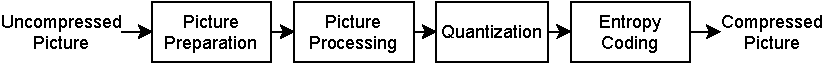
\includegraphics[width=0.9\textwidth]{data-compression-steps}
	\caption{Major steps of data compression.}{\label{fig:data-compression-steps}}
\end{figure}
%--------------------------Figure end -------------------

\textit{Decompression} is the inverse process of compression. Specific coders and decoders can be implemented very differently. Symmetric coding is characterized by comparable costs for encoding and decoding, which is especially desirable for dialogue applications. In an asymmetric technique, the decoding process is considerably less costly than the coding process. 

This is intended for applications where:
\begin{itemize}
	\item compression is performed once and 
	\item decompression takes place very frequently, or if the decompression must take place very quickly
\end{itemize}

For example, an audio-visual course module is produced once, but subsequently decoded by the many students who use it. The main requirement is real-time decompression. An asymmetric technique can be used to increase the quality of the compressed images.

\section{Basic Data Compression Techniques}
Compression basically employs redundancy in the data:
\begin{itemize}
	\item \textit{Temporal} in 1D data, 1D signals, audio, between video frames etc.
	\item \textit{Spatial} correlation between neighboring pixels or data items.
	\item \textit{Spectral} e.\ g.\ correlation between color or luminescence components. This uses the frequency domain to exploit relationships between frequency of change in data.
	\item \textit{Psycho-visual} exploit perceptual properties of the human visual system.
\end{itemize}

Compression methods can also be categorized in two broad ways:
\begin{enumerate}
	\item \textit{Lossless compression}:
	\begin{itemize}
		\item after decompression gives an exact copy of the original data.
		\item \textit{Example}: Entropy encoding schemes (Shannon-Fano, Huffman coding),	arithmetic coding, LZ/LZW algorithm (used in GIF image file format).
	\end{itemize}
	\item \textit{Lossy compression}:
		\begin{itemize}
		\item \textit{Example}: Transform coding — FFT/DCT based quantization used in	JPEG/MPEG differential encoding, vector quantization.
		\item Lossy methods are typically applied to high resolution audio, image compression.
		\item Have to be employed in video compression (apart from special cases).
	\end{itemize}
\end{enumerate}
 

%The hybrid compression techniques often used on audio and video data in multimedia systems are themselves composed of several techniques.
%
%The simplest techniques are based on \textit{interpolation} and \textit{subsampling}, whereby it is possible to make use of properties of the human eye or ear. For example, the eye is more sensitive to changes in brightness than to color changes. Therefore, instead of dividing an image into $ RGB $ (red, green, blue) components, a $ YUV $ representation can be used. The $ U $ and $ V $ components can then be sampled with lower horizontal and
%vertical resolution, a technique called \textit{subsampling}.

\subsection{Run-Length Coding}
\begin{itemize}
	\item Data often contains sequences of identical bytes. 
	\item By replacing these repeated byte sequences with the number of occurrences, a substantial reduction of data can be	achieved. 
	\item This is known as \textit{run-length coding}. 
\end{itemize}


A special marker $ M $ is needed in the data that does not occur as part of the data stream itself. 
To illustrate this, we define the exclamation mark `!' to be the `M-byte'. A single occurrence of an exclamation mark is interpreted as the `M-byte' during decompression. Two consecutive exclamation marks are interpreted as an exclamation mark occurring within the data.

The `M-byte' can thus be used to mark the beginning of a run-length coding. In the following example, the character \verb|C| occurs eight times in a row and is compressed to the three characters \verb|C!8| :

\[ \textrm{Uncompressed data:}\: \verb|ABCCCCCCCCDEFGGG|\]
\[ \textrm{Run-length coded:}\: \verb|ABC!8DEFGGG|\]


\subsection{Zero Suppression}
\begin{itemize}
	\item Run-length coding is a generalization of \textbf{zero suppression}, which assumes that just one symbol appears particularly often in sequences. 
	\item The blank (space) character in text is such a symbol; single blanks or pairs of blanks are ignored. 
\end{itemize}


\subsection{Pattern Substitution / Diatomic Encoding}
\begin{itemize}
	\item A technique that can be used for text compression substitutes single bytes for patterns that occur frequently. 
\end{itemize}


\subsection{Huffman Coding}
\begin{itemize}
	\item Huffman coding algorithm determines the optimal coding using the minimum number of bits. 
	\item Hence, the length (number of bits) of the coded characters will differ.
	\item The most frequently occurring characters are assigned to the shortest	code words. 
	\item A Huffman code can be determined by successively constructing a binary tree, whereby the leaves represent the characters that are to be encoded. 
	\item Every node contains the relative probability of occurrence of the characters belonging to the subtree beneath the node. 
	\item The edges are labeled with the bits $ 0 $ and $ 1 $.
\end{itemize}

\subsubsection*{Algorithm}
\begin{enumerate}
	\item Initialization: put all nodes in a list L, keep it sorted at all times (e.\ g.\ , ABCDE).
	\item Repeat until the list L has more than one node left.
	\begin{enumerate}[label=(\alph*)]
		\item From L pick two nodes having the lowest frequencies/probabilities, create a parent node of them.
		\item Assign the sum of the children’s frequencies/probabilities to the	parent node and insert it into L.
		\item Assign code 0/1 to the two branches of the tree, and delete the children from L
\end{enumerate}
\item Assign a codeword for each leaf based on the path from the root.
\end{enumerate}



%%%%%%%%%%%%%%%%%%%%%%%%%%%%%%%%%%%%%%%%%
%										%
%				FIGURE				   	%
%										%
%%%%%%%%%%%%%%%%%%%%%%%%%%%%%%%%%%%%%%%%%
\begin{figure}[ht!]
	\centering
	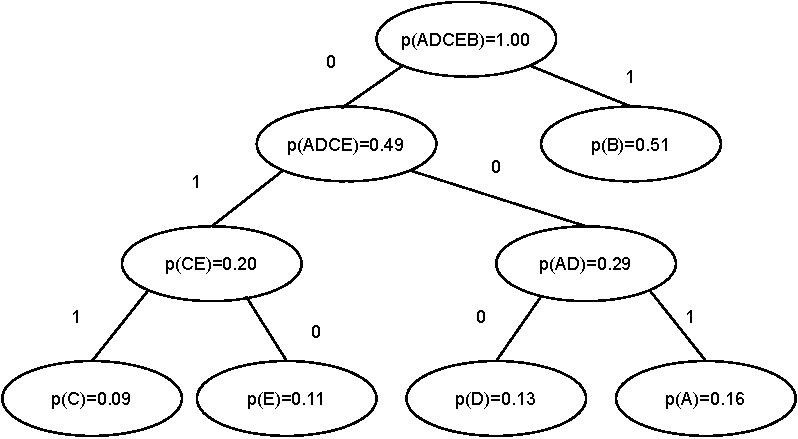
\includegraphics[width=0.8\textwidth]{huffman-coding}
	\caption{Example of a Huffman code represented as a binary tree}{\label{fig:huffman-coding}}
\end{figure}
%--------------------------Figure end -------------------

The following brief example illustrates this process:

\begin{enumerate}
	\item The letters $ A $, $ B $, $ C $, $ D $, and E are to be encoded and have relative probabilities of occurrence as follows:
	\[p(A)=0.16, p(B)=0.51, p(C)=0.09, p(D)=0.13, p(E)=0.11\]
	
	\item The two characters with the lowest probabilities, $ C $ and $ E $, are combined in the first binary tree, which gives the probability of $ 0.20 $ to their root node $ CE $. 
	
	\item Nodes with the following relative probabilities remain:
	\[p(A)=0.16, p(B)=0.51, p(CE)=0.20, p(D)=0.13\]
	
	The two nodes with the lowest probabilities are $ D $ and $ A $. These nodes are combined to form the leaves of a new binary tree. The combined probability of the
	root node $ AD $ is $ 0.29 $.
	
	
	\item Nodes with the following relative probabilities remain:
	\[p(AD)=0.29, p(B)=0.51, p(CE)=0.20\]
	
	The two nodes with the lowest probabilities are $ AD $ and $ CE $. These are combined into a binary tree. The combined probability of their root node $ ADCE $ is $ 0.49 $. 
	
	\item Two nodes remain with the following relative probabilities:
	\[p(ADCE)=0.49, p(B)=0.51\]
	
	These are combined to a final binary tree with the root node $ ADCEB $. 
	\item Figure {\ref{fig:huffman-coding}} shows the resulting Huffman code as a binary tree. The result is the following code words, which are stored in a table:
	\[w(A)=001, w(B)=1, w(C)=011, w(D)=000, w(E)=010\]
\end{enumerate}

Such a table could be generated for a single image or for multiple images together. The same table must be available for both encoding and decoding. 

\subsection{Arithmetic Coding}

\begin{itemize}
 \item Unlike Huffman coding, arithmetic coding does not code each symbol separately.
 \item Each symbol is instead coded by considering all prior data.
\end{itemize}

\subsection{Other Basic Techniques}
Apart from the compression techniques described earlier, some additional well
known techniques are used today:

\begin{itemize}
	\item Video compression techniques often use \textit{Color Look-Up Tables (CLUT)}.
	\item A simple technique for audio is silence suppression, whereby data is only encoded
	if the volume exceeds a certain threshold.
\end{itemize}

\section{Coding Standard JPEG, MPEG and DVI}

\subsection{JPEG}
\textit{Joint Photographic Experts Group (JPEG)} is an adaptive transformation coding techniques based on the Discrete Cosine Transform (DCT). In 1992, JPEG became an ISO International Standard. JPEG applies to color and gray-scaled still images.

Figure {\ref{fig:jpeg-compression-steps}} outlines the fundamental steps of JPEG compression in accordance with the general scheme illustrated in Figure {\ref{fig:data-compression-steps}}. JPEG defines several image compression modes by selecting different combinations of these steps.

\subsubsection*{JPEG Modes}
JPEG defines four modes, which themselves include additional variations:

\begin{itemize}
	\item The \textit{lossy}, sequential DCT-based mode (baseline process, base mode) must be
	supported by every JPEG decoder.
	\item The \textit{expanded lossy}, DCT-based mode provides a set of further enhancements to
	the base mode.
	\item The \textit{lossles}s mode has a low compression ratio and allows a perfect reconstruction
	of the original image.
	\item The \textit{hierarchical} mode accommodates images of different resolutions by using
	algorithms defined for the other three modes.
\end{itemize}

%%%%%%%%%%%%%%%%%%%%%%%%%%%%%%%%%%%%%%%%%
%										%
%				FIGURE				   	%
%										%
%%%%%%%%%%%%%%%%%%%%%%%%%%%%%%%%%%%%%%%%%
\begin{figure}[ht!]
	\centering
	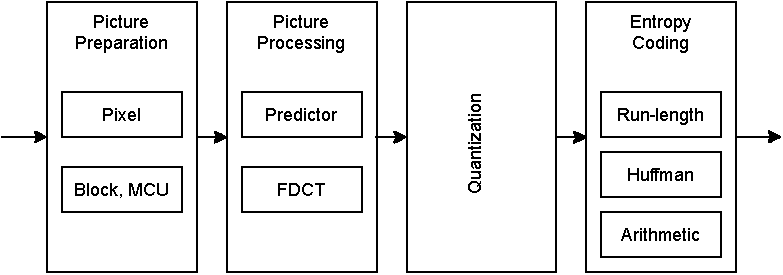
\includegraphics[width=0.8\textwidth]{jpeg-compression-steps}
	\caption[Steps of the JPEG compression technique]{Steps of the JPEG compression technique: summary of the different modes.}{\label{fig:jpeg-compression-steps}}
\end{figure}
%--------------------------Figure end -------------------



%\subsubsection{Image Preparation}
%For image preparation, JPEG specifies a very general image model that can
%describe most commonly used still image representations. For instance, the model is not
%based on three image components with $ 9-bit $ $ YUV $ coding and a fixed numbers of lines
%and columns. The mapping between coded color values and the colors they represent is
%also not coded. This fulfills the JPEG requirement of independence from image
%parameters such as image size or the image and pixel aspect ratios.
%
%An image consists of at least one and at most $ N=255 $ components or planes, as
%shown on the left side of Figure {\ref{fig:uncompressed-digital-image}}. These planes can be assigned to individual $ RGB $
%(red, green, blue) colors, or to the $ YIQ $ or $ YUV $ signals, for example.
%
%Each component is a rectangular array $ X_i \times Y_i $ of pixels (the samples). Figure {\ref{fig:jpeg-image-preparation}}
%shows an image with three planes, each with the same resolution.
%
%%%%%%%%%%%%%%%%%%%%%%%%%%%%%%%%%%%%%%%%%%
%%										%
%%				FIGURE				   	%
%%										%
%%%%%%%%%%%%%%%%%%%%%%%%%%%%%%%%%%%%%%%%%%
%\begin{figure}[H]
%	\centering
%	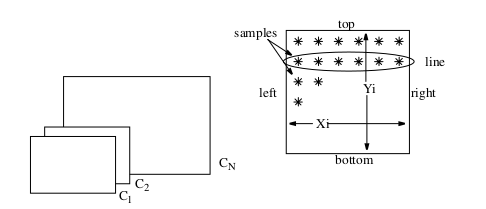
\includegraphics[width=0.8\textwidth]{uncompressed-digital-image}
%	\caption[Uncompressed digital image]{Digital uncompressed still image with the definition of the respective image components according to the JPEG standard}{\label{fig:uncompressed-digital-image}}
%\end{figure}
%%--------------------------Figure end -------------------
%
%The resolution of the individual components may be different. Figure {\ref{fig:jpeg-image-preparation-diff-res}} shows
%an image with three planes where the second and third planes have half as many columns as the first plane. A gray-scale image will, in most cases, consist of a single component, while an RGB color image will have three components with the same resolution (same number of lines $ Y_1 = Y_2 = Y_3  $and the same number of columns
%$ X_1 = X_2 = X_3 $ ). In JPEG image preparation, $ YUV $ color images with \textit{subsampling} of the
%chrominance components use three planes with $ Y_1 = 4Y_2 = 4Y_3 $ and $ X_1 = 4X_2 = 4X_3 $ .
%
%%%%%%%%%%%%%%%%%%%%%%%%%%%%%%%%%%%%%%%%%%
%%										%
%%				FIGURE				   	%
%%										%
%%%%%%%%%%%%%%%%%%%%%%%%%%%%%%%%%%%%%%%%%%
%\begin{figure}[H]
%	\centering
%	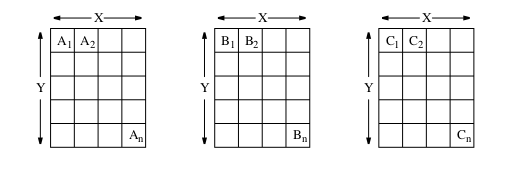
\includegraphics[width=0.8\textwidth]{jpeg-image-preparation}
%	\caption[Example of JPEG image preparation]{Example of JPEG image preparation with three components having the same resolution}{\label{fig:jpeg-image-preparation}}
%\end{figure}
%%--------------------------Figure end -------------------
%
%%%%%%%%%%%%%%%%%%%%%%%%%%%%%%%%%%%%%%%%%%
%%										%
%%				FIGURE				   	%
%%										%
%%%%%%%%%%%%%%%%%%%%%%%%%%%%%%%%%%%%%%%%%%
%\begin{figure}[H]
%	\centering
%	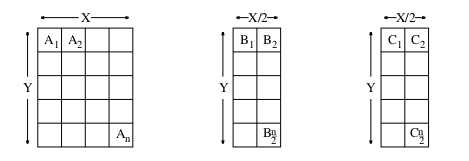
\includegraphics[width=0.8\textwidth]{jpeg-image-preparation-diff-res}
%	\caption[Example of JPEG image preparation having the different resolutions]{Example of JPEG image preparation with three components having the different resolutions}{\label{fig:jpeg-image-preparation-diff-res}}
%\end{figure}
%%--------------------------Figure end -------------------

\subsubsection*{Lossy Sequential DCT-Based Mode}
After image preparation, the uncompressed image samples are grouped into data units of $ 8 \times 8 $ pixels, as shown in Figure {\ref{fig:lossy-seq-dct}}; the order of these data units is defined by the MCUs. In this baseline mode, each sample is encoded using $ p=8bit $. Each pixel is an integer in the range $ 0 $ to $ 255 $.

%%%%%%%%%%%%%%%%%%%%%%%%%%%%%%%%%%%%%%%%%
%										%
%				FIGURE				   	%
%										%
%%%%%%%%%%%%%%%%%%%%%%%%%%%%%%%%%%%%%%%%%
\begin{figure}[h]
	\centering
	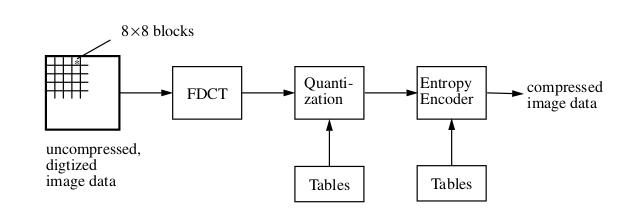
\includegraphics[width=\textwidth]{lossy-seq-dct}
	\caption[Steps of the lossy sequential DCT-based coding mode]{Steps of the lossy sequential DCT-based coding mode, starting with an
		uncompressed image after image preparation.}{\label{fig:lossy-seq-dct}}
\end{figure}
% --------------------------Figure end -------------------

%\paragraph*{Image Processing}
%The first step of image processing in the baseline mode, as shown in Figure {\ref{fig:lossy-seq-dct}}, is a transformation coding performed using the \textit{Discrete Cosine Transform (DCT)}. 

%The following \textit{FDCT (Forward DCT)} is then applied to each transformed pixel value:
%\[S_{vu}= \frac{1}{4}c_{u}c_{v}\sum_{x=0}^{7}\sum_{y=0}^{7}S_{yx}\cos \frac{(2x+1)u\pi}{16}\cos\frac{(2y+1)v\pi}{16}\]
%
%where, 
%\[c_{u}, c_{v}= \frac{1}{\sqrt{2}} \: \textrm{for} \: u, v=0; \: \textrm{otherwise}\: c_{u}, c_{v}=1\]
%
%Altogether, this transformation must be carried out 64 times per data unit. The result is $ 64 $ coefficients $ S_{vu} $.
%
%Due to the dependence of DCT on the Discrete Fourier
%Transform (DFT), which maps values from the time domain to the frequency domain,
%each coefficient can be regarded as a two-dimensional frequency.
%
%\subsubsection{Quantization}
%Image processing is followed by the quantization of all DCT coefficients; this is a
%lossy process. For this step, the JPEG application provides a table with 64 entries, one
%for each of the 64 DCT coefficients. This allows each of the 64 coefficients to be
%adjusted separately. The application can thus influence the relative significance of the
%different coefficients. Specific frequencies can be given more importance than others
%depending on the characteristics of the image material to be compressed. The possible
%compression is influenced at the expense of achievable image quality.
%
%The table entries $ Q_{vu} $ are integer values coded with $ 8 bits $. Quantization is
%performed according to the formula:
%\[sq_{vu}=round\frac{S_{vu}}{Q_{vu}}\]
%
%The greater the table entries, the coarser the quantization. Dequantization is per-
%formed prior to the IDCT according to the formula:
%\[R_{vu}=Sq_{vu} \times Q_{vu}\]
%Quantization and dequantization must use the same tables.
%
%\subsubsection{Entropy Encoding}
%During the next step, either the initial step of entropy encoding or preparation for
%the coding process, the quantized DC-coefficients are treated differently than the quan-
%tized AC-coefficients. The processing order of all coefficients is specified by the zig-zag
%sequence.
%
%JPEG uses Huffman coding and arithmetic coding as entropy encoding methods.
%For the lossy sequential DCT-based base mode, only Huffman
%encoding is allowed. In both methods, a run-length encoding of zero values is first
%applied to the quantized AC-coefficients. Additionally, non-zero AC-coefficients as
%well as the DC-coefficients are transformed into a spectral representation to further
%compress the data. The number of bits required depends on the value of each coefficient. Non-zero AC-coefficients are represented using between 1 and 10 bits. For the
%representation of DC-coefficients, a higher resolution of 1 bit to a maximum of 11 bits
%is used.

\paragraph*{Steps of JPEG Image Compression}
\begin{steps}
	\item \textit{Splitting}: The input image is divided into a small block which is having $ 8 \times 8 $ dimensions. This dimension is sum up to 64 units. Each unit of the image is called \textit{pixel}.
	\item \textit{Color Space Transform}: JPEG uses $ [Y,Cb,Cr] $ model instead of using the $ [R,G,B] $ model. $ RGB $ is converted into $ YCbCr $.
	\begin{itemize}
		\item Y is for brightness, 
		\item Cb is color blueness, and 
		\item Cr for color redness. 
	\end{itemize}
	\item \textit{Apply DCT}: After the conversion of colors, it is forwarded to DCT. DCT uses a cosine function and does not use complex numbers. It converts information which are in a block of pixels from the spatial domain to the frequency domain.
	\item \textit{Quantization}  is used to reduce the number of bits per sample.
	\item \textit{Serialization}: The zigzag scan is used to map the $ 8 \times8 $ matrix to a $ 1 \times 64 $ vector. Zigzag scanning is used to group low-frequency coefficients to the top level of the vector and the high coefficient to the bottom. 
	\item \textit{Vectoring}: The different pulse code modulation (DPCM) is applied to the DC component. DPCM encodes the difference between the current block and the previous block.
	\item \textit{Encoding}: Run Length Encoding (RLE) is applied to AC components. This is done because AC components have a lot of zeros in it. It encodes in a pair of \texttt{(skip, value)} in which \texttt{skip} is non-zero value and \texttt{value} is the actual coded value of the non-zero components.	
\end{steps}

\subsection{MPEG}
MPEG was developed and defined by ISO/IEC JTC1/SC 29/WG 11 to cover motion video as well as audio coding. 


\subsubsection{Video Encoding}
MPEG supports four types of image coding. In order to achieve a high compression ratio, temporal redundancies of successive images need to be exploited. Fast random access requires that images be coded individually. Hence the following image types are distinguished:

\paragraph{I-Frames (Intra-coded frames)}
%P-frames (predictive-coded frames)
	\begin{itemize}
	\item Are coded without using information about other frames.
	\item An $ I $-frame is treated as a still image. Here, MPEG	falls back on the results of JPEG.
	\item Unlike JPEG, real-time compression must be possible.
	\item The compression rate is thus the lowest within MPEG. 
	\item $ I $-frames form the anchors for random access.
	\item $ I $-frames are encoded by performing a DCT on the $ 8\times8 $ blocks defined within the macro blocks.
	\end{itemize}




\paragraph{P-Frames (Predictive-coded frames)}
\begin{itemize}
	\item Require information about previous I and/or $ P $	frames for encoding and decoding. 
	\item Decoding a $ P $-frame requires decompression of the last $ I $ frame and any intervening $ P $-frames. 
	\item In return, the compression ratio is considerably higher than for I frames. 
	\item A $ P $-frame allows the following $ P $-frame to	be accessed if there are no intervening $ I $ frames.
\end{itemize}


\paragraph{B-frames (Bidirectionally predictive-coded frames}
\begin{itemize}
	\item Require information from previous and following $ I $ and/or $ P $ frames. 
	\item $ B $-frames yield the highest compression ratio attainable in MPEG. 
	\item A $ B $-frame is defined as the difference from a prediction based on a previous and a following $ I $ or $ P $-frame. 
	\item It cannot serve as a reference for prediction coding of other frames.
\end{itemize}


\paragraph{D-frames (DC coded frames}
\begin{itemize}
	\item Are intraframe-coded and can be used for efficient fast forward. 
	\item During the DCT, only the DC-coefficients are coded; the AC coefficients are ignored.
\end{itemize}





\noindent Figure \ref{fig:mpeg-frames} shows a sequence of $ I $, $ P $, and $ B $-frames. This example illustrates the prediction for the first $ P $-frame and the bidirectional prediction for a $ B $-frame. The order in which the images are presented differs from the actual decoding order if $ B $-frames are present in an MPEG-coded video stream.


The pattern of $ I $, $ P $, and $ B $-frames in a sequence is determined by the MPEG application. For random access, the ultimate resolution would be attained by encoding the
entire stream using $ I $-frames. The highest compression rate can be achieved by using as many $ B $-frames as possible. For practical applications, the sequence \verb|IBBPBBPBBIBBPBBPBB...| has proven to be useful. This permits random access with a resolution of nine still images (i.\ e.\ , about $ 330ms $) and still provides a very good compression ratio. Every 15 images includes one $ I $-frame.

%%%%%%%%%%%%%%%%%%%%%%%%%%%%%%%%%%%%%%%%%
%										%
%				FIGURE				   	%
%										%
%%%%%%%%%%%%%%%%%%%%%%%%%%%%%%%%%%%%%%%%%
\begin{figure}[ht!]
	\centering
	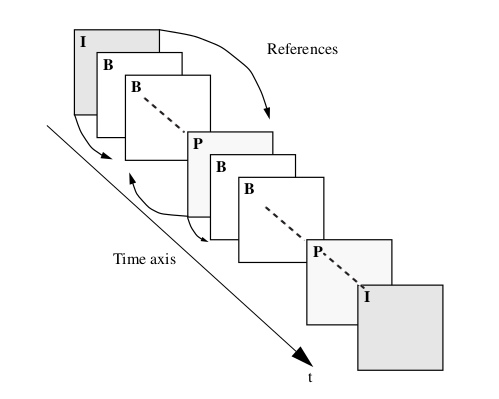
\includegraphics[width=0.7\textwidth]{mpeg-frames}
	\caption[Types of individual images in MPEG]{Types of individual images in MPEG: I, B, and P frames.}{\label{fig:mpeg-frames}}
\end{figure}
%--------------------------Figure end -------------------


%\subsubsection*{Quantization}
%Concerning quantization, it should be noted that AC-coefficients of $ B $ and $ P $-frames are usually very large values, whereas those of $ I $-frames are very small. Thus,
%MPEG quantization adjusts itself accordingly. If the data rate increases too
%much, quantization becomes more coarse. If the data rate falls, then quantization is
%performed with finer granularity.

\subsubsection{Audio Coding}
MPEG audio coding uses the same sampling frequencies as Compact Disc Digital Audio (CD-DA) and Digital Audio Tape (DAT), i.\ e.\ , $ 44.1 kHz $ and $ 48 kHz $, and additionally, $ 32kHz $ is available, all at $ 16 bits $.

Three quality levels (layers) are defined with different encoding and decoding complexity. An implementation of a higher layer must be able to decode the MPEG audio signals of lower layers.

%\paragraph*{Psychoacoustic Model}
%The noise level in each sub-band is determined using a psycho-acoustic model.

Similar to two-dimensional DCT for video, a transformation into the frequency domain is applied for audio. The Fast Fourier Transform (FFT) is a suitable technique.
As shown in Figure \ref{fig:mpeg-audio-encoding}:
\begin{itemize}
	\item The relevant portion of the spectrum is divided into 32 non-overlapping subbands. 
	\item The audio signal is thus split into 32 subbands. 
	\item Different components of the spectrum can then be quantized differently. 
	\item In parallel with the actual FFT,the noise level in each subband is determined using a psychoacoustic model. 
	\item At a higher noise level, a coarser quantization is performed. 
	\item A lower noise level results in finer quantization.
	\item In the first and second layers, the appropriately quantized spectral components are simply PCM-encoded. 
	\item The third layer additionally performs Huffman	coding.
\end{itemize}

\begin{figure}[ht!]
	\centering
	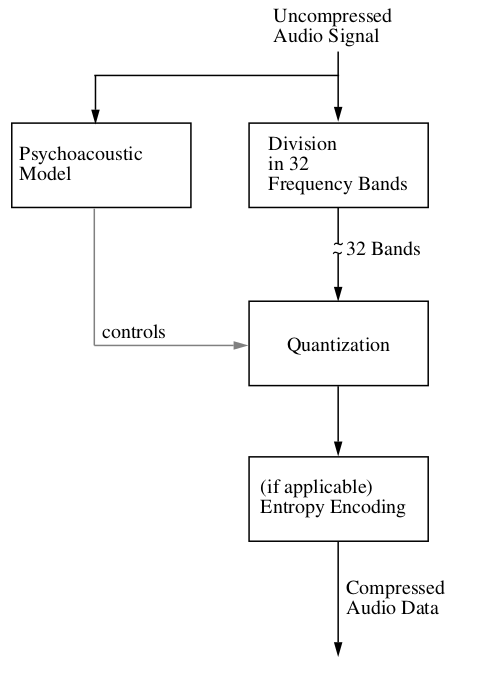
\includegraphics[width=0.6\textwidth]{mpeg-audio-encoding}
	\caption{MPEG audi encoding.}
	\label{fig:mpeg-audio-encoding}
\end{figure}

Audio coding can be performed on stereo sound, a single channel, or two independent channels. MPEG provides for two types of stereo sound. 
\begin{itemize}
	\item In the first case, two channels are processed completely independently. 
	\item In the joint stereo mode, MPEG achieves a higher compression ratio by exploiting redundancies between the two	channels.
\end{itemize}

\subsection{DVI}
\textit{Digital Video Interactive}(DVI) is a technology that includes coding algorithms. The fundamental components are a VLSI chip set for the video subsystem, a well-specified data format for audio and video files, an application user interface to the audio-visual kernel (AVK, the kernel software interface to the DVI hardware) and compression, as well as decompressing, algorithm. 

DVI can process\textit{ data, text, graphics, still images, video} and \textit{audio}. The original essential characteristic was the asymmetric technique of video compression and decompression known as Presentation-Level Video (PLV).

\subsubsection{Audio and Still Image Encoding}
Audio signals are digitized using $ 16 bits $ per sample and are either PCM-encoded or compressed using the Adaptive Differential Pulse Code Modulation (ADPCM) technique. Thereby, a reduction to about four bits per sample is achieved at a quality corresponding to stereo broadcasting.

When encoding still images, different video input formats can be used. These can be composite, as well as component video signals like, RGB. In the case of an RGB signal, the color of each pixel is split into portions of the three colors of the spectrum-red, green and blue - and each color is processed separately.

\subsubsection{Video Encoding}
For motion video encoding DVI distinguishes two techniques with different resolutions and dissimilar goals:

\begin{itemize}
	\item \textit{Presentation-Level Video (PLV)} is characterized by its better quality. This is achieved at the expense of a very time-consuming asymmetric compression
	performed by specialized compression facilities.
	
	\item \textit{Real-Time Video (RTV)} is a symmetric compression technique that works with hardware and software and can be performed in real-time.
\end{itemize}


Where,
\begin{enumerate}
	\item \textit{Asymmetric coding} requires considerably more effort for encoding than for decoding. Compression is carried out once, whereas decompression is performed many times. A typical application area is retrieval systems. 
	
	\item \textit{Symmetric compression} is characterized by a comparable effort for the compression and decompression processing.
\end{enumerate}
 % Chapter-5: Data Compression
\chapter{Optical Storage Media}
Conventional magnetic data carriers in the form of hard disks or removable disks are traditionally used in computers as secondary storage media. These offer low average access time and provide enough capacity for general computer data at an acceptable price. However, audio and video data, even in compressed form, place heavy demands on available storage capacity. The storage cost for continuous media is thus substantial unless other data carriers are used.

Optical storage media offer higher storage density at a lower cost. The \textit{audio compact disc} (CD) has been commercially successful in the consumer electronics industry as the successor to \textit{long-playing records} (LPs) and is now a mass-produced product.

\section{Basic Technology}
\begin{itemize}
	\item In optical storage media, information is represented by using the intensity of laser light reflected during reading. 
	\item A laser beam having a wave length of about $ 780nm $ can be focused to a resolution of approximately $ 1 \mu m $. 
	\item In a polycarbonate substrate layer, there are depressions, called \textit{pits}, corresponding to the	data to be encoded. 
	\item The areas between the pits are called \textit{lands}.
\end{itemize}

Figure {\ref{fig:cd-pits-lands}} shows a sectional view through an optical disc, running lengthwise along a data track. The pits and lands are represented schematically in the middle of the figure.
%%%%%%%%%%%%%%%%%%%%%%%%%%%%%%%%%%%%%%%%%
%										%
%				FIGURE				   	%
%										%
%%%%%%%%%%%%%%%%%%%%%%%%%%%%%%%%%%%%%%%%%
\begin{figure}[ht!]
	\centering
	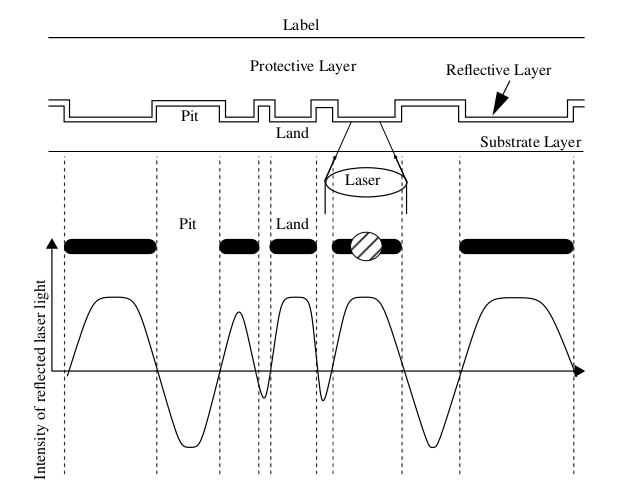
\includegraphics[width=0.8\textwidth]{cd-pits-lands}
	\caption[Sectional view of an optical disc]{Sectional view of an optical disc along the data track. Schematic representation of the layers (top), the ``lands'' and the ``pits'' (middle), and the signal waveform (bottom).}{\label{fig:cd-pits-lands}}
\end{figure}
%--------------------------Figure end -------------------

\begin{itemize}
	\item The substrate layer is smooth and coated with a thin, reflective layer. 
	\item The laser beam is focused at the height of the reflective layer from the substrate level. 
	\item The reflected beam thus has a strong intensity at the lands. 
	\item The pits have a depth of $ 0.12\mu m $ from the substrate surface. 
	\item Laser light hitting pits will be lightly scattered, that is, it will be reflected with weaker intensity. 
	\item The signal waveform shown schematically at the bottom of Figure {\ref{fig:cd-pits-lands}} represents the intensity of the reflected laser light; the horizontal
	line represents a threshold value. 
	\item The laser in the figure is currently sampling a land.
\end{itemize}

According to Figure {\ref{fig:cd-pits-lands}}, a Compact Disc (CD) consists of:
\begin{multicols}{2}
	\begin{itemize}
		\item the label,
		\item the protective layer,
		\item the reflective layer and
		\item the substrate.
	\end{itemize}
\end{multicols}

%%%%%%%%%%%%%%%%%%%%%%%%%%%%%%%%%%%%%%%%%
%										%
%				FIGURE				   	%
%										%
%%%%%%%%%%%%%%%%%%%%%%%%%%%%%%%%%%%%%%%%%
\begin{figure}[ht!]
	\centering
	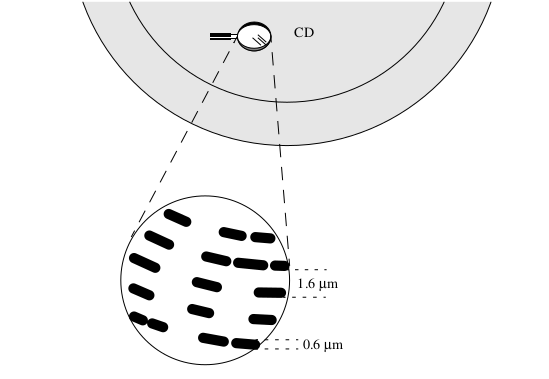
\includegraphics[width=0.7\textwidth]{data-on-cd}
	\caption[Data on a CD as an example of an optical disc]{Data on a CD as an example of an optical disc. Track with ``lands'' and ``pits''.}{\label{fig:data-on-cd}}
\end{figure}
%--------------------------Figure end -------------------

\begin{multicols}{2}
	\begin{itemize}
		\item An optical disc consists of a sequential arrangement of pits and lands within a track. 
		\item The pits and lands represent data on the surface (see Figure {\ref{fig:data-on-cd}}).
		\item All the information on an optical disc is placed on one track. 
		\item The stored information can thus be played back at a continuous data rate
		\item A track is in the form of a spiral. 
		\item In the case of a CD, the spacing between adjacent coils of the spiral—the track pitch is $ 1.6 \mu m$. 
		\item The track width of the pits is $ 0.6 \mu m $, though their lengths can vary. 
	\end{itemize}
\end{multicols}

The light source of the laser can be positioned at a distance of approximately $ 1 mm $ from the disk surface and thus does not touch the disk directly, or float on an air cushion. This reduces wear and tear on the components used and increases the life of the device.

\section{Video Disc Fundamentals}
\begin{itemize}
	\item Video discs in the form of \textit{LaserVision} are used for the reproduction of motion picture and audio data. 
	\item The data are stored on the disc in an analog-coded format, and
	\item the sound and picture quality are excellent. 
	\item \textit{LaserVision} discs have a diameter of approximately $ 30cm $ and store approximately $ 2.6Gbytes $.
\end{itemize}


Motion pictures are frequency-modulated on the video disc, and the audio signal is mixed with the modulated video signal. Figure {\ref{fig:video-disc}} shows the principle used to record data. 
\begin{itemize}
	\item The important information of the mixed audio-video signal is the temporal	sequence of the zero transitions. 
	\item Each zero transition corresponds to a change between a pit and a land on the disc.
	\item Such a change can occur at any time, and is written to the disc in a non-quantized form, that is, the pit length is not quantized. 
	\item This method is thus time-continuous and can be characterized as analog.
\end{itemize}


%%%%%%%%%%%%%%%%%%%%%%%%%%%%%%%%%%%%%%%%%
%										%
%				FIGURE				   	%
%										%
%%%%%%%%%%%%%%%%%%%%%%%%%%%%%%%%%%%%%%%%%
\begin{figure}[ht!]
	\centering
	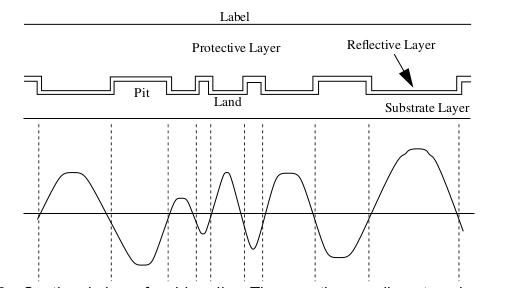
\includegraphics[width=0.8\textwidth]{video-disc}
	\caption[Sectional view of a video disc]{Sectional view of a video disc. Time-continuous discrete value coding.}{\label{fig:video-disc}}
\end{figure}
%--------------------------Figure end -------------------

The video disc was conceived as a Read Only Memory. Since then, many different write-once optical storage systems have come out, known as Write Once Read Many (WORM). An example is the Interactive Video Disc, which operates at Constant Angular Velocity (CAV). On each side, up to 36 minutes of audio and video data at 30 frames per second can be stored and played back. Alternatively, approximately 54,000 studio quality still images can be stored per side.

WORMs have the following special properties:
\begin{itemize}
	\item The term \textit{Media overflow} refers to problems that can occur when a WORM disc is almost full.
	
	\item \textit{Packaging} refers to problems stemming from the fixed block structure of WORMs.
	
	\item \textit{Revision} refers to the problem of subsequently marking areas as invalid.
\end{itemize}

\section{CD Audio, CD ROM and Extended Architecture}
\subsection[CD Audio]{Compact Disc Digital Audio}
The Compact Disc Digital Audio (CD-DA) was developed jointly by N.\ V.\ Philips and the Sony Corporation \textit{for storing audio data}. The basic technology of the CD-DA was developed by N.\ V.\ Philips.

\subsubsection{Technical Basics}
\begin{itemize}
	\item CDs have a diameter of $ 12cm $ and are played at a \textit{Constant Linear Velocity (CLV)}.
	\item The number of rotations per time unit thus depends on the radius of the data currently being sampled. 
	\item The spiral-shaped CD track has approximately 20,000 windings.
\end{itemize}


Information is stored according to the principle depicted in Figure {\ref{fig:cd-pits-lands}} and Figure {\ref{fig:cd-da}}, whereby the length of the pits is always a multiple of $ 0.3 \mu m $. A change from pit to land or from land to pit corresponds to the coding of a $ 1 $ in the data stream. If there is no change, a $ 0 $ is coded.

%%%%%%%%%%%%%%%%%%%%%%%%%%%%%%%%%%%%%%%%%
%										%
%				FIGURE				   	%
%										%
%%%%%%%%%%%%%%%%%%%%%%%%%%%%%%%%%%%%%%%%%
\begin{figure}[ht!]
	\centering
	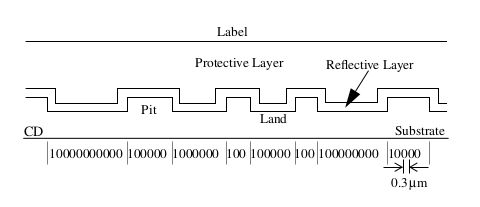
\includegraphics[width=0.8\textwidth]{cd-da}
	\caption[``Pits'' and ``lands'']{``Pits'' and ``lands''. Discrete time, discrete value storage.}{\label{fig:cd-da}}
\end{figure}
%--------------------------Figure end -------------------

\subsubsection{Audio Data Rate}
The audio data rate can easily be derived from the given sampling rate of
$ 44,100Hz $ and the $ 16bit $ linear quantization. The stereo audio signal is pulse code modulated, and the data rate is as follows:
\begin{flalign*}
	& \textrm{Audio data rate}_{CD-DA}\\
	& = 16 \frac{bits}{sample \:value} \times 2 \: channels \times 44,100 \frac{sample \:values}{s \times channel} \\
	& = 14,11,200 \times \frac{bits}{s} \\
	& = 14, 11,200 \times \frac{bits/s}{8 bits /byte} \\ 
	& = 14, 11, 200 \times \frac{\cancel{bits}}{s} \times \frac{byte}{8\cancel{bits}}\\
	& = 14,11,200 \times \frac{byte}{8s}\\
	& = 1,76,400 \times \frac{byte}{s}\\
	& = 176.4\frac{Kbytes}{s} \: \textnormal{(\textnp{१, ७६, ४०० लाई १,००० ले भाग गरेकाे}})  \\
	& \cong  172.3 \frac{Kbytes}{s} \: \textnormal{(\textnp{१, ७६, ४०० लाई १,०२४ ले भाग गरेकाे})} &&
\end{flalign*}
\noindent Where, \textit{$\cong$ means ``is congruent to (that is the equality up to a displacement)"}.\\

Analog long-playing records and casette tapes have a signal-to-noise ratio of
approximately $ 50 $ to $ 60dB $. The quality of the CD-DA is substantially higher. As a rule
of thumb, one can assume $ 6dB $ per bit used during the sampling process. Given $ 16bit $ linear sampling:
\begin{flalign*}
	S/N_{CD-DA} \cong 6\frac{dB}{bit} \times 16 bits  = 96dB
\end{flalign*}
The signal-to-noise ratio is exactly $ 98dB $.

\subsubsection*{Capacity}
The play time of a CD-DA is at least \textit{74 minutes}. Using this value, the capacity of a CD-DA can easily be determined. The capacity given below applies only to storage
used for audio data, without, for example, taking into account data used for error correction:
\begin{flalign*}
    \textrm{Capacity}_{CD-DA} 
    & = 74 min \times 14,11,200 \frac{bits}{s} \\
    & = 74 \times 60 \times 14,11,200 \frac{bits}{s} \\
    & = 6,26,57,28, 000 \frac{bits}{s}\\
   & = 6,26,57,28, 000 bits \times \frac{1}{8\frac{bits}{byte}} \times \frac{1}{1,024\frac{bytes}{Kbyte}} \times \frac{1}{1,024\frac{Kbytes}{Mbyte}} \\
   & \cong 747 Mbytes 
\end{flalign*}

\subsection{CD-ROM}
The Compact Disc Read Only Memory (CD-ROM) was conceived as a storage medium for general computer data, in addition to uncompressed audio data. Further, CD-ROM technology was intended to form the basis for the storage of other media. It was specified by N.\ V.\ Philips and the Sony Corporation in the \textit{Yellow Book} and later accepted as an ECMA standard.

CD-ROM tracks are divided into \textit{audio} (corresponding to CD-DA) and \textit{data} types. Each track may contain exclusively data of one type. A CD-ROM can contain both types of tracks. In a mixed mode disc, the data tracks are usually located at the beginning of the CD-ROM, followed by the audio tracks.

\subsubsection{Blocks}
Since CD-ROMs store general computer data, they require better error correction and higher resolution random access to data units than are specified for CD-DA. A CD-DA has an error rate of $ 10^{-8} $ and allows random access to individual tracks and index points.

This data unit is called a \textit{block}, meaning the \textit{physical block}. In the ISO 9660 standard, there also exists the notion of a \textit{logical block}. The logical block has similar properties to the sectors of other media and file system. 

A CD-ROM block consists of the $ 2,352 bytes $ of a CD-DA block. Thus the $ de facto $ CD-DA standard can serve as the basis for the de facto CD-ROM standard.

Of the $ 2,352 bytes $ of a block, $ 2,048 bytes $ (computer data) or $ 2,336 bytes $ (audio data) are available for user data. The remaining bytes are used for identification for random access and for another error correction layer that further reduces the error rate.

Figure {\ref{fig:cd-rom-data-hierarchy}} shows the data hierarchy of a CD-ROM or CD-DA.

$ 75 blocks $ per second are played back, each consisting of $ 32 frames $. Each frame is
$ 73.5 bytes $ ($ 588 bits $).
\begin{flalign*}
   \textrm{Blocks} &= 14,11, 200 \frac{bits}{s} \times \frac{1}{75}s \times \frac{1}{8bits/byte} \\
   & = 2, 352 bytes 
\end{flalign*}

%cd-rom-data-hierarchy

%%%%%%%%%%%%%%%%%%%%%%%%%%%%%%%%%%%%%%%%%
%										%
%				FIGURE				   	%
%										%
%%%%%%%%%%%%%%%%%%%%%%%%%%%%%%%%%%%%%%%%%
\begin{figure}[hb!]
	\centering
	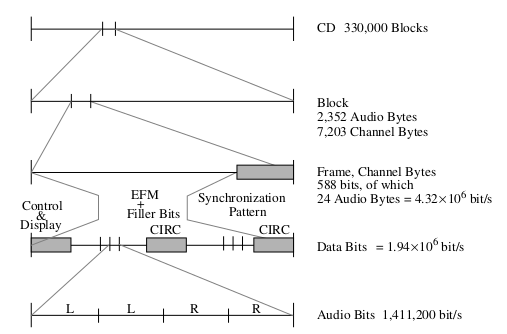
\includegraphics[width=0.8\textwidth]{cd-rom-data-hierarchy}
	\caption[CD-ROM data hierarchy]{CD-ROM data hierarchy. Audio blocks as on a CD-DA}{\label{fig:cd-rom-data-hierarchy}}
\end{figure}
%--------------------------Figure end -------------------

\subsubsection{Modes}
The CD-ROM specification was defined with the goal of storing uncompressed CD-DA data and computer data, as well as serving as the basis for other media. This is
achieved by using two CD-ROM modes:
\begin{multicols}{2}
\begin{itemize}
	\item \textit{mode 1} and
	\item \textit{mode 2}
\end{itemize} 
\end{multicols}


An additional mode $ 0 $, where all $ 2,336 $ user data bytes are set to zero, serves to separate storage areas.

\paragraph*{CD-ROM Mode 1}
\begin{itemize}
	\item CD-ROM mode 1 is used to store computer data, as shown in Figure {\ref{fig:cd-rom-mode-1}}. 
	\item Of the $ 2,352 $ total bytes in each block, $ 2,048 bytes $ are available for storing information.
\end{itemize}

%%%%%%%%%%%%%%%%%%%%%%%%%%%%%%%%%%%%%%%%%
%										%
%				FIGURE				   	%
%										%
%%%%%%%%%%%%%%%%%%%%%%%%%%%%%%%%%%%%%%%%%
\begin{figure}[H]
	\centering
	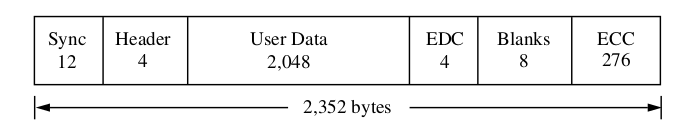
\includegraphics[width=0.8\textwidth]{cd-rom-mode-1}
	\caption[CD-ROM mode 1]{CD-ROM mode 1 block (sector) layout.}{\label{fig:cd-rom-mode-1}}
\end{figure}
%--------------------------Figure end -------------------
To be more exact, the $ 2,352 bytes $ can be broken down into the following groups:

\begin{itemize}
	\item $ 12 bytes $ for synchronization as the start-of-block indicator,
	\item $ 4 bytes $ for the header. This contains an unambiguous block identifier.
	\begin{itemize}
		\item The first	two bytes contain minutes and seconds, respectively; 
		\item the third byte contains the block number, 
		\item while the fourth byte identifies the mode.
	\end{itemize}
	
	\item $ 2,048 bytes $ of user data,
	\item $ 4 bytes $ for error detection,
	\item $ 8 $ unused bytes, and
	\item $ 276 bytes $ for error correction, whereby an error rate of $ 10^{-12} $ can be achieved.
\end{itemize}

A CD-ROM contains $ 3,33,000 blocks $ to be played in$  74 minutes $. The capacity of a CD-ROM with all blocks in \textit{mode 1} can be calculated as follows:

\begin{flalign*}
     {Capacity}_{{CD-ROM}_{Mode \:1}} 
    & = 3,33,000 blocks \times 2, 048 \frac{bytes}{block} \\
    & = 68,19,84,000 bytes \\
    & = 68,19,84,000 bytes \times \frac{1}{1,024 \frac{bytes}{Kbyte}} \times \frac{1}{1,024 \frac{Kbytes}{Mbyte}} \\
    &  \cong 650 Mbytes &
\end{flalign*}

The data rate in \textit{mode 1} is:
\begin{flalign*}
	  {Rate}_{{CD-ROM}_{Mode \:1}}  
     & = 2, 048 \frac{bytes}{block} \times 75 \frac{blocks}{s}\\
     & = 153.6 \frac{Kbytes}{s} \\
     & \cong 150 \frac{Kbytes}{s} 
\end{flalign*}


\paragraph*{CD-ROM Mode 2}
\begin{itemize}
	\item CD-ROM mode 2 serves as the basis for additional specifications for storage of other media.
	\item A block in this mode is shown in Figure {\ref{fig:cd-rom-mode-2}}. 
	\item Of the $ 2,352 $ total bytes in each block, $ 2,336 bytes $ are available for storing information.
\end{itemize}

%%%%%%%%%%%%%%%%%%%%%%%%%%%%%%%%%%%%%%%%%
%										%
%				FIGURE				   	%
%										%
%%%%%%%%%%%%%%%%%%%%%%%%%%%%%%%%%%%%%%%%%
\begin{figure}[H]
	\centering
	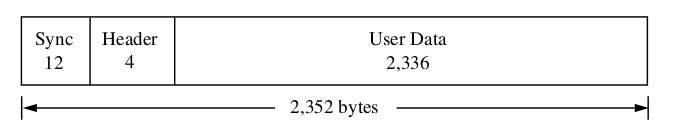
\includegraphics[width=0.8\textwidth]{cd-rom-mode-2}
	\caption[CD-ROM mode 2]{CD-ROM mode 2 block (sector) layout.}{\label{fig:cd-rom-mode-2}}
\end{figure}
%--------------------------Figure end -------------------

The synchronization and header are dealt with as in mode 1. The additional error correction is left out.

The capacity of a CD-ROM with all blocks in mode 2 can be calculated as follows:
\begin{flalign*}
	{Capacity}_{{CD-ROM}_{Mode \:2}} 
	& = 3,33, 000 blocks \times 2,336 \frac{bytes}{block} \\
	& = 77,78,88, 000 bytes \\
	& = 741.8518 Mbytes
\end{flalign*}

The data rate in \textit{mode 2} is:
\begin{flalign*}
	{Rate}_{{CD-ROM}_{Mode \:2}}  
	& = 2,336 \frac{bytes}{block} \times 75 \frac{blocks}{s}\\
	& = 175.2 \frac{Kbytes}{s} \\
\end{flalign*}


\subsection{CD ROM Extended Architecture}
\begin{itemize}
	\item The \textit{Compact Disc Read Only Memory Extended Architecture} (CD-ROM/XA), is based on the CD-ROM specification.
	\item Was established by N.\ V.\ Philips, the Sony Corporation, and Microsoft. 
	\item The main motivation was to address the inadequate consideration paid until then to concurrent output of multiple media.
\end{itemize}


The \textit{Red Book} specifies a track for uncompressed audio data. The \textit{Yellow Book} specifies tracks for computer data using CD-ROM \textit{mode 1} (Figure {\ref{fig:cd-rom-mode-1}}) and tracks for compressed media using CD-ROM \textit{mode 2} (Figure {\ref{fig:cd-rom-mode-2}}).

\begin{itemize}
	\item CD-ROM/XA uses CD-ROM \textit{mode 2} in order to define its own blocks and additionally defines a sub-header that describes each block (sector) as shown in Figure {\ref{fig:cd-xa-form-1}} and Figure {\ref{fig:cd-xa-form-2}}. 
	\item This makes it possible to interleave different media using only \textit{mode 2} blocks, since these can contain different media. 
	\item The individual CD-ROM/XA data	streams are separated during playback.
\end{itemize}





\subsubsection*{Form 1 and Form 2}
CD-ROM/XA differentiates blocks with form 1 and form 2 formats, similar to the CD-ROM modes:

\subsubsection{Form 1}
\begin{itemize}
	\item The XA format form 1 in CD-ROM mode 2 provides improved error detection and correction. 
	\item Like CD-ROM mode 1, 4 bytes are needed for error detection and $ 276 bytes $ for error correction.
	\item Unlike CD-ROM mode 1, the 8 bytes	unused in CD-ROM mode 1 are used for the subheader. 
	\item Figure \ref{fig:cd-xa-form-1} shows a block (sector), where  $2,048 bytes$ are used for data.
\end{itemize}

%%%%%%%%%%%%%%%%%%%%%%%%%%%%%%%%%%%%%%%%%
%										%
%				FIGURE				   	%
%										%
%%%%%%%%%%%%%%%%%%%%%%%%%%%%%%%%%%%%%%%%%
\begin{figure}[ht!]
	\centering
	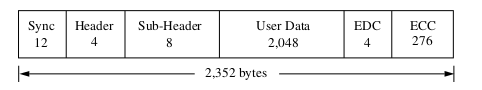
\includegraphics[width=0.8\textwidth]{cd-xa-form-1}
	\caption[Sector layout (1) for CD-ROM/XA according to the ``Green Book''.]{Sector layout (1) for CD-ROM/XA according to the ``Green Book''. Data layout of a CD-ROM block in mode 2, form 1}{\label{fig:cd-xa-form-1}}
\end{figure}
%--------------------------Figure end -------------------


\subsubsection{Form 2}

\begin{itemize}
	\item The XA format form 2 in CD-ROM mode 2 allows a 13 percent increase in actual data capacity, to $ 2,324 bytes $ per block, at the expense of error handling.
	\item Form 2 blocks can be used to store compressed data of various media, including audio and video data.
\end{itemize}

%%%%%%%%%%%%%%%%%%%%%%%%%%%%%%%%%%%%%%%%%
%										%
%				FIGURE				   	%
%										%
%%%%%%%%%%%%%%%%%%%%%%%%%%%%%%%%%%%%%%%%%
\begin{figure}[ht!]
	\centering
	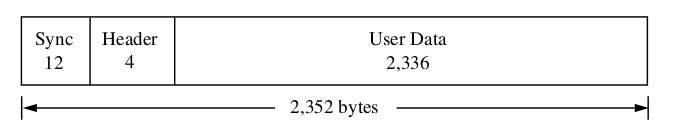
\includegraphics[width=0.8\textwidth]{cd-rom-mode-2}
	\caption[Sector layout (2) for CD-ROM/XA according to the ``Green Book''.]{Sector layout (2) for CD-ROM/XA according to the ``Green Book''. Data layout of a CD-ROM block in mode 2, form 2.}{\label{fig:cd-xa-form-2}}
\end{figure}
%--------------------------Figure end -------------------

\noindent On a CD-DA, CD-ROM, or mixed mode disc, a track always consists of homogeneous data, meaning exclusively audio or computer data. It is thus not possible for the
computer to, for example, concurrently read uncompressed audio data and computer data. 


\subsubsection*{Advantage of CD-ROM/XA}
\begin{itemize}
	\item Blocks of different media can be stored in one track since they are all coded in CD-ROM mode 2.
\end{itemize}

\section{Principles of CD-WO and CD-MO}
\section*{CD Write-Once}
So far, all the CD technologies considered do not allow the user to write to the disk. Thus, the application scope is limited. This has led research laboratories
to develop, besides the \textit{Read Only Storage Media}, compact disks that can be recorded once or several times.

The \textit{Compact Disk Write Once} (CD-WO), like WORM (Write Once Read Many), allows the user to write once to a CD and afterwards to read it many times. CD-WO is specified in the second part of the \textit{Orange Book}.

\subsection{Principle of CD-WO}
Figure {\ref{fig:cd-wo}} shows a cross-section of a CD-WO, vertical to the disk surface and data track. In the case of read-only CDs, the substrate (a polycarbonate) lies directly next to the reflection layer.

%%%%%%%%%%%%%%%%%%%%%%%%%%%%%%%%%%%%%%%%%
%										%
%				FIGURE				   	%
%										%
%%%%%%%%%%%%%%%%%%%%%%%%%%%%%%%%%%%%%%%%%
\begin{figure}[h]
	\centering
	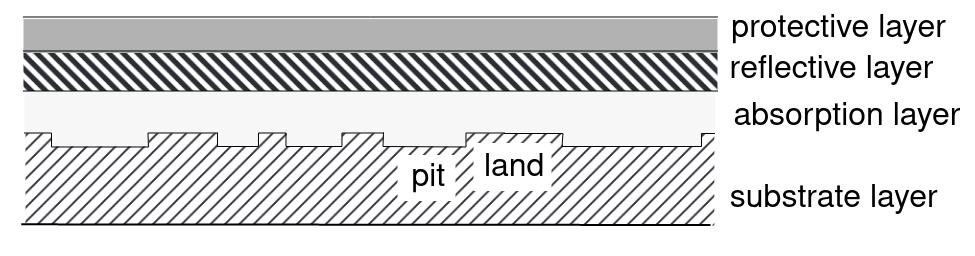
\includegraphics[width=0.8\textwidth]{cd-wo}
	\caption{Cross-section of a CD-WO disc.}\label{fig:cd-wo}
\end{figure}
%--------------------------Figure end -------------------

%\begin{multicols}{2}
\begin{itemize}
	\item In the case of a CD-WO, an \textit{absorption layer} exists between the substrate and the reflection layer. 
	\item This layer can be irreversibly modified through strong thermal influence, which changes the reflection properties	of the laser beams.

		\item In its original state, a CD-WO player recognizes a track consisting of lands. 
		\item The absorption layer in the pre-grooved track is heated to above $ 250 \degree C $ with a laser three to four times the intensity of a reading player. 
		\item Hence, the absorption layer changes such that the reflection of the laser light now corresponds to a pit. 
		\item This method determines the most remarkable property of the CD-WO: its data can be played by any devices which are meant only for read-only CDs.
%\end{multicols}
\end{itemize}

%\subsection*{Sessions}
%\begin{itemize}
%	\item All CD systems described so far assume that a \textit{lead-in area} exists before the actual
%	data area of a CD, and  
%	\item A \textit{lead-out area} exists after the actual data of a CD
%	\item The content is written in a \textit{table of contents} in the lead-in area
%	\item Each player needs this table of contents to position the player correctly
%	\item In the case of writing to a CD-WO, this lead-in area with the table of contents can be
%	overwritten only after the entire write activity is complete
%	\item This means that the actual data of a CD-WO must be written before the table of contents is created
%	\item Therefore, the principle of seueral sessions was introduced, as shown in Figure {\ref{fig:cd-wo-sessions}}
%	\item Bach session has its own lead-in area and lead-out area
%	\item During one write activity, all data for a session are written together with their table of contents, after which the disk can be played on other device
%	\item Thereby the structure of a CD can be extended up to a maximal 99 session
%	\item However, because of the space requirement for lead-in and lead-out areas, at most 46 sessions can be stored
%	\item Each session consists again of its lead-in area, the data area and lead-out area
%	\item Until 1992, all available devices could read only one session
%	\item CD-WOs with only one session are called \textit{regular} CD-WOs. 
%	\item A CD-WO with more than one session is called a \textit{hybrid} CD-WO
%\end{itemize}
%
%
%%%%%%%%%%%%%%%%%%%%%%%%%%%%%%%%%%%%%%%%%%
%%										%
%%				FIGURE				   	%
%%										%
%%%%%%%%%%%%%%%%%%%%%%%%%%%%%%%%%%%%%%%%%%
%\begin{figure}[H]
%	\centering
%	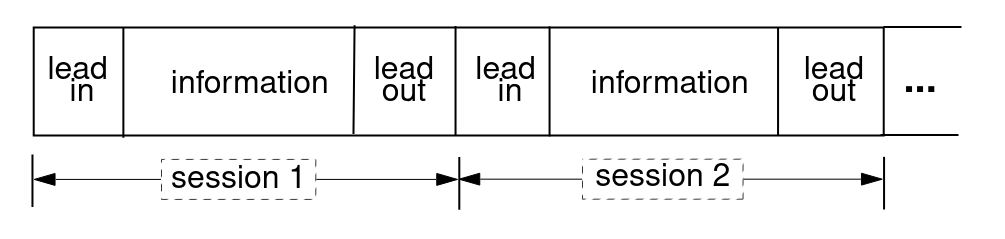
\includegraphics[width=\textwidth]{cd-wo-sessions}
%	\caption{Cross-section of a CD-WO disc}\label{fig:cd-wo-sessions}
%\end{figure}
%%--------------------------Figure end -------------------

\subsection*{CD Magneto Optical}
The Compact Disc Magneto Optical (CD-MO), specified in the first part of the \textit{Orange Book}, has a high storage capacity and allows the CD to be written multiple times.

%%%%%%%%%%%%%%%%%%%%%%%%%%%%%%%%%%%%%%%%%
%										%
%				FIGURE				   	%
%										%
%%%%%%%%%%%%%%%%%%%%%%%%%%%%%%%%%%%%%%%%%
\begin{figure}[ht!]
	\centering
	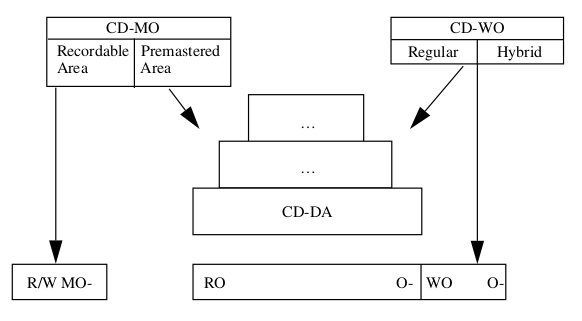
\includegraphics[width=0.8\textwidth]{cd-mo}
	\caption[CD-WO and CD-MO in relation to other CD technologies.]{CD-WO and CD-MO in relation to other CD technologies: structure in multiple layers.}\label{fig:cd-mo}
\end{figure}
%--------------------------Figure end -------------------


\subsection[Principle of CD-MO]{Principle of CD Magnetic-Optical}
\begin{itemize}
	\item The magneto-optical technique is based on the principle that at higher temperatures, a weak magnetic field is needed to polarize the dipoles in certain materials. 
	\item The block (sector) to be written is heated to above $150 \degree C$. 
	\item At the same time, a magnetic field about ten times the strength of the Earth’s magnetic field is applied. 
	\item At this point, the material’s dipoles are polarized towards this magnetic field.
	\item A pit is coded with a downwards-facing magnetic north pole. 
	\item A land is coded using the opposite orientation.
\end{itemize}

In order to erase a block (sector), the area around the block is subjected to a constant magnetic field while it is heated.

If the CD is illuminated by a laser, the polarization of the light changes depending on the magnetization of the CD. In this way, the information can be read.

\subsection*{Areas of a CD-MO}
\begin{itemize}
	\item A CD-MO consists of an optional read-only area and the actual rewritable area.
	\item The read only area (premastered area in Figure {\ref{fig:cd-mo}}) contains data written on the disc in a format specified for this purpose. 
	\item In Figure {\ref{fig:cd-mo}}, this relationship is indicated using the arrows between the premastered area of a CD-MO and the read only technologies. 
	\item Thus, the read only area can be read using existing playback devices.
\end{itemize}

 The rewritable area of a CD-MO cannot be read using existing CD-DA, CD-ROM, CD-ROM/XA, or CD-WO devices due to the fundamentally different technology used for reading and writing. Figure {\ref{fig:cd-mo}} shows the relationships between this recordable area and the underlying magneto-optical technology. This technology is thus incompatible with all the other CD technologies.

\newpage\thispagestyle{empty} % Chapter-6: Optical Storage Media
\chapter{Documents, Hypertext and MHEG}

\section{Document Architecture and Multimedia Integration}
Document is a set of structured information which may be present in various media and may be generated or input at the time of presentation. A document is used by humans and is available for editing in a computer.

\subsection*{Documents}
\begin{itemize}
	\item A \emph{multimedia document} is characterized by information which is coded in at least one continuous (time-dependent) and one discrete (time-independent) medium. \item The integration of various media is possible because of close relationships between information units. 
	\item This is also called \emph{synchronization}. 
	\item A multimedia document should be viewed in the environment of tools, data abstractions, basic concepts, and document architectures.
	
\end{itemize}

%Continuous and discrete data are still viewed and treated in many different ways. A text within an editing program is treated as a type of programming language (type character), and a motion picture is manipulated in the same editing program only via library calls. The levels of view are different, and so are the manipulation options. The goal of abstraction of multimedia data is an integrated, uniform way of describing and handling all media. This means an essential reduction of the complexity with regard to setting up and maintaining such programs. Abstractions of multimedia data serve as a basis for writing code for many different types of multimedia programs, in particular editors and other document processing tools.


Fundamental system concepts use abstractions of multimedia data, they serve as a concept for information architectures, and they can be implemented by use of tools. In this respect, the terms \textit{document architecture} and \textit{information architecture} are synonymous.


\subsection{Document Architecture}
\begin{itemize}
	\item Exchange of documents means the communication of both content and structure. 
	\item In addition to common communication protocols, it also requires the use of a document architecture. 
	\item This includes standardized architectures, such as SGML (Standard Generalized Markup Language).
	\item Such information architectures use data abstractions and their concepts for specification and implementation. 
	\item A document architecture describes the interplay of models (see Figure {\ref{fig:document-arch}}).
\end{itemize}


Figure {\ref{fig:document-arch-component}} shows a multimedia information architecture characterized by the internal interplay of individual information units from discrete and continuous media.


In the interplay of models, the manipulation describes operations that can be performed on multimedia information. 
\begin{itemize}
	\item \textit{Communication} and \textit{storage} define the protocols used to exchange this information between different computers and the format used to store data.
	\item The \textit{presentation} of multimedia information collects relationships between individual parts of information, which have to be maintained in the presentation of this information. 
\end{itemize}

Not every architecture includes all properties or models mentioned here.




%%%%%%%%%%%%%%%%%%%%%%%%%%%%%%%%%%%%%%%%%
%										%
%				FIGURE				   	%
%										%
%%%%%%%%%%%%%%%%%%%%%%%%%%%%%%%%%%%%%%%%%
\begin{figure}[ht!]
	\centering
	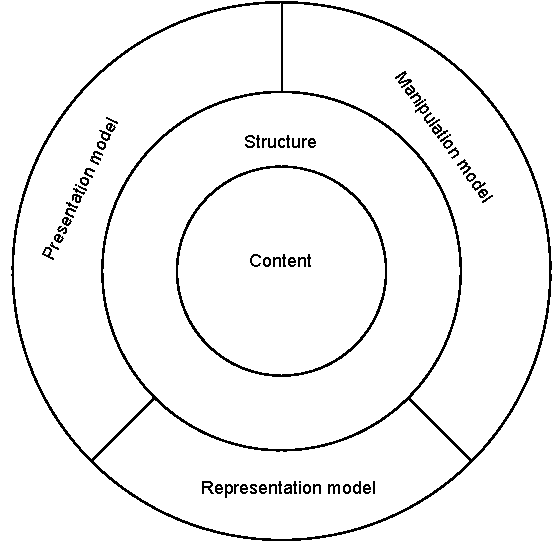
\includegraphics[width=0.6\textwidth]{document-arch}
	\caption{Architecture of documents and their components.}{\label{fig:document-arch}}
\end{figure}
%--------------------------Figure end -------------------

%%%%%%%%%%%%%%%%%%%%%%%%%%%%%%%%%%%%%%%%%
%										%
%				FIGURE				   	%
%										%
%%%%%%%%%%%%%%%%%%%%%%%%%%%%%%%%%%%%%%%%%
\begin{figure}[hb!]
	\centering
	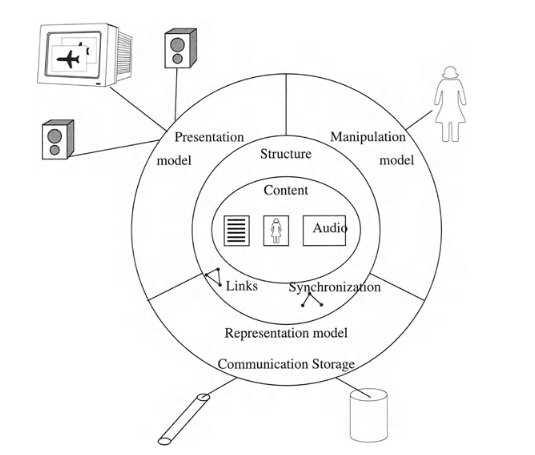
\includegraphics[width=0.8\textwidth]{document-arch-components}
	\caption{Architecture of multimedia documents and their components.}{\label{fig:document-arch-component}}
\end{figure}
%--------------------------Figure end -------------------


\subsection{Multimedia Integration}
See Section \ref{sec:notion-of-synchronization}, Page No.\ \pageref{sec:notion-of-synchronization}.
\section{Hypertext, Hypermedia and Multimedia}
A book or an article in paper form has a pre-determined structure and is present in sequential form. However, we can read specific sections in a targeted way without having read previous sections. Authors normally assume sequential reading, so that many sections are based on knowledge previously acquired. Both fictional literature and movies always assume a purely sequential reception. Scientific literature can consist of independent chapters. However, in this context too, sequential reading is assumed.


Technical documentation (e.\ g.\, manuals) consists often of a collection of relatively independent information units. A lexicon or reference book about the Airbus, for example, is generated by several authors and always only parts are read sequentially. There also exist many cross-references in such documentations which lead to
multiple searches at different places for the reader. Here, an electronic help facility, consisting of information links, can be very significant.

Figure \ref{fig:hypertext-data} shows an example of such a concatenation or linking. 

\begin{figure}[ht!]
	\centering
	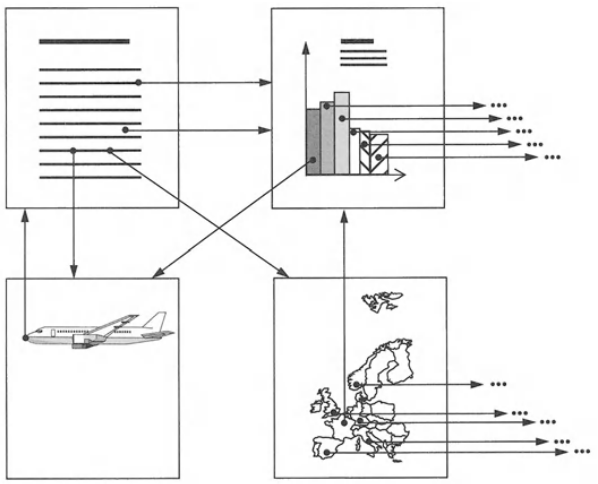
\includegraphics[width=0.7\textwidth]{hypertext-data}
	\caption[Hypertext data.]{Hypertext data. An example of linking information of different media.}
	\label{fig:hypertext-data}
\end{figure}

\begin{multicols}{2}
\begin{enumerate}
	\item Each arrow specifies a relationship between logical information units (LDUs). 
	\item A piece of text (top left in the figure) includes a reference to the climb properties of an aircraft. 
	\item These properties are demonstrated in a video sequence (bottom left in the figure). 
	\item At a different location in the same text, the sales subsidiaries located in Europe are listed (and the list is visualized in a graphical map, shown at the bottom right in the figure).
	\item More information about each sales point can be viewed by selecting that location in the graphical	map. 
	\item A special piece of information about the number of different aircrafts sold in the Paris subsidiary is shown in the form of a bar chart (top right in the figure). \item Internally, all information contained in this chart are present only in tabular form. 
	\item The left bar refers to the aircraft, which can be seen in a video.
\end{enumerate}

\end{multicols}


\subsection*{Non-linear Linking of Information}
\begin{multicols}{2}
	\begin{enumerate}
	\item The most important property of hypertext and hypermedia is non-linear information linking. 
	\item There is a reading sequence, but the reader also decides about the reading path. 
	\item For example, when browsing in a lexicon, the reader can start with the term hypertext and then use the cross-reference systems to jump to a description of AppleTalk. 
	\item Using this association, based on reference links, the	author of the information normally determines the links.
	\end{enumerate}
\end{multicols}


A hypertext structure is a \textit{graph}, consisting of \textit{nodes} and \textit{edges}.
\begin{multicols}{2}
	\begin{enumerate}[label=(\alph*)]
		\item The \textit{nodes} are the actual information units. 
		\item They are, for example, the text elements, individual graphics, audio or video LDUs. 
		\item The \textit{edges} form a relationship between different information units. They are called \textit{reference} or \textit{link}. 
		\item A reference is normally a directed edge. 
		\item All linking elements contain information.
	\end{enumerate}
\end{multicols}

Figure {\ref{fig:hyper-multi}} shows the relationship between multimedia, hypertext, and hypermedia.

%%%%%%%%%%%%%%%%%%%%%%%%%%%%%%%%%%%%%%%%%
%										%
%				FIGURE				   	%
%										%
%%%%%%%%%%%%%%%%%%%%%%%%%%%%%%%%%%%%%%%%%
\begin{figure}[ht!]
	\centering
	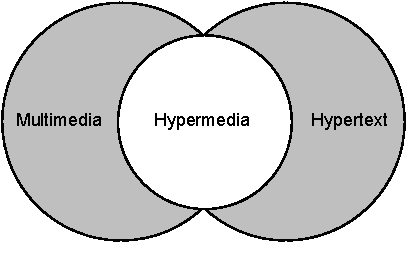
\includegraphics[width=0.5\textwidth]{hyper-multi}
	\caption{Hypertext, hypermedia and multimedia, and their relationships.}{\label{fig:hyper-multi}}
\end{figure}
%--------------------------Figure end -------------------


\subsection[Hypertext]{Hypertext System}
\begin{multicols}{2}
	\begin{itemize}
		\item A hypertext system is essentially characterized by non-linear linkage of information. 
		\item Pointers/References connect the nodes. 
		\item The data of various nodes can be present in one medium or several media. 
		\item In a pure text system, only the text sections are	linked. 
		\item The term \textit{hypertext} means that several media can be linked, in addition to simple	text.
	\end{itemize}
\end{multicols}


\subsection[Multimedia]{Multimedia System}
\begin{multicols}{2}
	\begin{itemize}
		\item A multimedia system contains information encoded at least in one continuous and one discrete medium. 
		\item For example, when text data are connected by a non-linear link, then this belongs to the hypertext category. 
		\item A video conference with simultaneous transmission of text and graphics from a conventional linear program for document editing is a multimedia application.
	\end{itemize}
\end{multicols}


\subsection[Hypermedia]{Hypermedia System}
\begin{multicols}{2}
	\begin{itemize}
		\item A hypermedia system includes the non-linear linkage of information which is normally present in either a continuous or a discrete medium. 
		\item For example, text and video data within a non-linear linkage structure belong to the hypermedia, multimedia, and hypertext categories.
	\end{itemize}
\end{multicols}



Figure {\ref{fig:hyper-multi}} shows that each hypermedia system belongs to the hypertext category and is a multimedia system at the same time. It forms the intersection set of both multimedia and hypertext.

\subsubsection*{Application Areas of of Hypermedia}
\begin{multicols}{2}
	\begin{itemize}
		\item \textit{Computer-based applications} to include the help function of modern graphical interface.
		\item \textit{Commercial applications} include repair and operating instructions.
		\item \textit{Intellectual applications} include organization of ideas, brainstorming, or text creation.
		\item \textit{Education and research} are areas with a large potential for improvement by use of continuous media.
		\item The \textit{entertainment industry} has used hypertext for information or guiding systems for tourists and interactive science-fiction movies.
	\end{itemize}
\end{multicols}


\section{Systems: Architecture, Nodes and Pointers}

\subsection{Architecture}
The architecture of a hypertext system can be divided into \textit{three levels} with different functionalities.
%\begin{center}
%	\begin{framed}
%			\begin{nepali}
%			\textbf{नाेट}: याे शीर्षक भित्र level अथवा layer भनेमा एउटै हुन् भन्ने बुझिन्छ। अरुकाे नाेटमा layer लेखेकाे भएपनि दुवै एकै हाे भनेर मान्ने।
%		\end{nepali}
%	\end{framed}
%%	%\end{center}

\begin{multicols}{2}
	\begin{enumerate}
		\item \textit{Presentation Level}
		\item \textit{Hypertext Abstract Machine} 
		\item \textit{Storage/Databse Level}
	\end{enumerate}
\end{multicols}

\subsubsection[Presentation Level]{Top Level: Presentation Level}
\begin{multicols}{2}
	\begin{itemize}
		\item The top or \textit{presentation level} accommodates all functions relating to the user interface. 
		\item This level is used to map nodes and references to the user interface. 
		\item The user interface offers the visualization of one or several sections. 
		\item This level determines the data to be displayed and how it should be represented based on the structure and the display chosen by the user.
		\item This level is also responsible for the control of all inputs.
	\end{itemize}
\end{multicols}


\subsubsection[Hypertext Abstract Machine]{Hypertext Abstract Machine (HAM)}
\begin{multicols}{2}
	\begin{itemize}
		\item The HAM is located between the presentation level (level One) and the storage level (level Two).
		\item This level takes database-like functions to store multimedia data within a local or distributed environment from the lower level. 
		\item HAM level does not have to worry about the input and output of the upper level. 
		\item HAM knows the structure of a document, and it disposes of knowledge about the references and their attributes. 
		\item This means that the HAM level builds the data structure, or an object hierarchy, for document management. 
	\end{itemize}
\end{multicols}

Compared to the other two levels, the HAM level is the one least dependent on the system. This means that it is also best suitable for standardization.

\subsubsection[Storage Level]{Storage/Database Level}
\begin{multicols}{2}
\begin{itemize}
	\item The \textit{storage level} (also called \textit{database level}) forms the lowest level. 
	\item It includes all functions relating to the storage of data, i.\ e.\ , secondary storage management. 
	\item In this respect, the specific properties of the different sets of data from discrete and continuous media are important. 
	\item This is also the level where capabilities of traditional database systems, i.\ e.\ , persistence, multi-user operation
	(synchronization, locking), and error recovery (transaction concept), are expected. 
	\item The nodes and pointers of a hypertext document are processed as data objects without any special semantics.
\end{itemize}
\end{multicols}



\noindent Unfortunately, most implementations of hypertext systems do not clearly separate these different levels. The reasons are normally a shorter development phase, a more efficient implementation, and shortcomings in most generally available multimedia interfaces for the lowest level.

\subsection{Nodes}
A node is an information unit (LDU) in a hypertext document. The most important distinguishing criterion between different implementations is the maximum data quantity a node can accommodate.

\subsubsection{Maximum Data Quantity}

\begin{multicols}{2}
	\begin{itemize}
		\item The \textit{maximum data quantity} contained in a node can be limited to match the screen size.
		\item A motion picture sequence and an audio clip could be limited to a duration of, for example, 36 seconds.
	\end{itemize}
\end{multicols}
An author is forced eventually to distribute logical connected text content to several cards, although it is not desired. Applying it to video clips and audio passages, it would mean that the close interconnection among the distributed sequences could get lost easily. An advantage is the \textit{clear and intuitive environment}.


\subsubsection{Unlimited Data Quantity}
\begin{multicols}{2}
	\begin{itemize}
		\item One alternative are window-based systems with a basically \textit{unlimited data quantity} per node. 
		\item Forward and backward scrolling of pages is offered analogous to other windows at the user interface. 
		\item \textit{Intermedia} is such a system. Intermedia does not limit the duration of continuous media with regard to the data volume its nodes can accommodate.
	\end{itemize}
\end{multicols}

This means that single nodes can have very different lengths and still appear equal-ranking. The presentation of additional information also uses two different methods at the user interface: 

	\begin{itemize}
			\item First, there is a way to switch between the nodes,
			\item and second, a node uses the mechanisms known from window-based systems for \textit{scrolling}.
	\end{itemize}

	

\noindent A secondary criterion concerns the \textit{time when a piece of information is created}. In general, the author can specify the entire contents of the nodes while creating a document.

\subsection{Pointers}
%\begin{center}
%	\begin{framed}
%	\begin{nepali}
%		नाेटः यस शीर्षक भित्र pointer अथवा reference भन्नु एउटै हाे।
%	\end{nepali}
%	\end{framed}
%\end{center}
\textit{Pointers/References} form the edges in a hypertext graph. Hypertext systems differ by various edge criteria. One of the first questions to ask here would be: \textit{Which information is contained in a pointer?}

\begin{multicols}{2}
	\begin{itemize}
		\item \textit{Simple pointers} connect two nodes of a graph without containing any information themselves. They merely establish a relationship between those nodes.
		
		\item \textit{Typified pointers} connect two nodes and include additional information. A label is assigned to each reference. This label is used to create comments to each reference (e.\ g.\ , author and creation date).
	\end{itemize}
\end{multicols}


Another Property of the pointers is connected to the question: \textit{What does the pointer mean?} Often, pointers with very different meanings are used together. This usage complicates the understanding. The author of a hypertext should know about this problem and use unambiguous pointers. The following relations can be expressed through pointers:

\begin{multicols}{2}
	\begin{itemize}
		\item \textit{To be} - $ A $ is part of $ B $. This represents a quantity relationship.
		\item \textit{To present} - $ A $ is an example of $ B $, or $ A $ demonstrates $ B $. This case uses an example to state a fact.
		\item \textit{To produce} - $ A $ produces $ B $, or $ B $ is a result of $ A $. This case can describe consequences from a fact in more detail.
		\item \textit{To require or required by} - $ A $ requires $ B $, $ B $ needs $ A $. This relationship expresses
		an absolute necessity.
		\item \textit{To own} - $ A $ owns $ B $, or $ A $ is associated to $ B $. This relationship expresses an ownership.
		\item \textit{To include} - $ A $ includes $ B $, or $ A $ consists of $ B $, or $ A $ occurs in $ B $. This relationship
		represents different meanings of an inclusion.
		\item \textit{Similarity} - $ A $ is similar to $ B $, $ A $ is different from $ B $, $ A $ replaces $ B $, $ A $ is the alternative to $ B $. This relationship expresses similarities.
	\end{itemize}
	
\end{multicols}

Another fundamental property of pointers can be described by the following question: \textit{Who states a pointer?} We distinguish as follows:
\begin{multicols}{2}
	\begin{itemize}
		\item \textit{Implicit References}: A relationship between nodes can be created automatically by a hypertext system. The author specifies only the algorithms used to create the references. 
		
		\item \textit{Explicit References}: All references are created by the author.
	\end{itemize}
\end{multicols}


A reference can be created at different times, which leads us to the question: \textit{When is the target of a pointer stated?}

\begin{multicols}{2}
	\begin{itemize}
		\item In the classical case, a reference is created during the creation of the hypertext document, and both the origin and the target node are specified. When editing the	document, the author specifies explicitly how the information units should be
		linked.
		
		\item A target node can be determined when the reference is used, i.\ e.\ , while the document is read. The author specifies an algorithm to be used to create the references, while the references are determined when the user reads the context. The system 	calculates the target node.
	\end{itemize}
\end{multicols}

In most systems, however, each pointer has exactly one origin and one target node. On the other hand, we could ask the following question:
\begin{itemize}
	\item \textit{ What direction does the pointer have?} and
	\item \textit{What is the number of outgoing pointers?}
\end{itemize}


\begin{multicols}{2}
	\begin{itemize}
		\item The direction is normally unidirectional, while the system itself supports \textit{backtracking}. This means that we would always get back on track.
		\item The alternative would be bidirectional references, which means that we would have to highlight or mark both the target nodes and the anchors. When introducing bidirectional references, it could easily happen that several nodes refer to the same target nodes. This means that these references have to be explicitly distinguished at the target node.
		\item The same applies to references leading from one origin to several target nodes.
		\item Most systems support unidirectional references with only one target node each. This is easier to understand and to implement.
	\end{itemize}
\end{multicols}

As our last question, we would have to deal with the appearance of an anchor on the user interface. More specifically, we can ask the following question: \textit{How can a reference be represented?}

\subsubsection*{Anchors}
The forward movement in linear sorted documents is called a \textit{navigation} through the graph. At the user interface, the origin of references has to be marked, so that the user can jump from one information unit to another. This origin of a pointer is called an \textit{anchor}.

\begin{multicols}{2}
	\begin{itemize}
		\item A \textit{media-independent representation} can be realized with general graphic elements, like the ones commonly used for selection, e.\ g.\ , buttons. The information about the target node should be included in such an element:
		\begin{itemize}
			\item If the target node is a piece of text, then an abbreviated, descriptive (verbose) summary of the contents could be represented. 
			\item For a single image, the respective image contents could be displayed on the screen in the form of a miniature or
			``thumbnail''. 
			\item A visual representation of video contents could be implemented in the form of moving icons (micons\footnote{ A micon is a reduced motion picture, representing a characteristic part of the video sequence of the target node.}). 
			\item If the contents of the target node consist of audio information, then the audio contents should be represented visually. For a music clip,	for example, this could be a picture of the composer
		\end{itemize}
	
	\item For \textit{text}, we could emphasize single words, paragraphs, or text sections of different lengths. A pointer can be positioned on a section emphasized in this way, so that the user could double-click the highlighted section to display the target node referred to by the pointer
	\item For \textit{single images}, specific graphic objects or simply areas are defined as selection	objects. A specific marking can occur through a color or stripe.
	\item For \textit{motion pictures}, media-independent representations of anchors are the preferred method.
	\item For audio, we would always have to use a media-independent solution. In this case, we would use a brief descriptive text or a single image of the size of an icon.
	\end{itemize}
\end{multicols}

\subsection*{Tools}
A hypertext system consists of several required tools:
\begin{multicols}{2}
	\begin{itemize}
		\item One or more \textit{editors} are used to edit information from various media.
		\item \textit{Search tools} are used to find information.
		\item A \textit{browser} is used to obtain a short and clear representation of the nodes and edges.
		\item During the \textit{navigation} through a document, a proper support of the phenomena \textit{Getting Lost in the Hyperspace} is needed. A \textit{backtracking} and clear representation	of the whole structure with respect to the actual position should be available.
	\end{itemize}
\end{multicols}

%\subsubsection*{Editors}
%
%
%\subsubsection*{Search tools}
%
%
%\subsubsection*{Browser}
%
%
%\subsubsection*{Navigation and Backtracking}


\section{Architecture: SGML and ODA and MHEG}
\subsection[SGML]{SGM Document Architecture}
The \textit{Standard Generalized Markup Language} (SGML) has been promoted mainly by US publishing companies. The authors provide text, i.\ e.\, contents. They use a uniform markup format to describe titles, tables, and other document elements, without actually describing the document's look (e.\ g.\ , fonts or line spacing). The final layout is determined by the publisher.

\begin{multicols}{2}
	\begin{itemize}
		\item The basic idea is that the author uses tags to mark specific text parts. 
		\item SGML defines the look of these tags, but it does not define where they should occur, or what meaning they should have. 
		\item Instead, user groups agree on the meaning of such tags.
		\item SGML offers a frame that can be used to describe the syntax in a way specific to a user group within an object-oriented system. 
		\item Classes and objects, hierarchies of classes and objects, inheritance, and embedded methods (processing instructions) can be used in	the specification.
		\item SGML defines the syntax but no semantics.
	\end{itemize}
\end{multicols}


The following example shows the use of SGML in a text document:
\begin{lstlisting}[language=xml, frame=single]
<title>Multimedia Application</title>
<course>BCA</course>
<semester>VIII</semester>
<author>Jeevan Poudel</author>
<year>2077</year>
<summary>This is for BCA  ...
...
\end{lstlisting}

\subsection*{Using SGML}
%%%%%%%%%%%%%%%%%%%%%%%%%%%%%%%%%%%%%%%%%
%										%
%				FIGURE				   	%
%										%
%%%%%%%%%%%%%%%%%%%%%%%%%%%%%%%%%%%%%%%%%
\begin{figure}[ht!]
	\centering
	\includegraphics[width=0.7\textwidth]{sgml-doc-processing}
	\caption{SGML document processing, from information to representation.}{\label{fig:sgml-doc-processing}}
\end{figure}
%--------------------------Figure end -------------------

The handling process for an SGML document shown in Figure {\ref{fig:sgml-doc-processing}} splits the processing job into two processes:
\begin{itemize}
	\item The \textit{formatter} knows the meaning of the tags, and uses these tags to produce a formatted document. 
	
	\item The \textit{parser} uses the tags contained in the document in combination with the appropriate document type.
\end{itemize}

Tags can be used to define the structure of a document, which normally includes the association of some parts of the layout. It is based on the common context between the creator of the document and the formatting process, but not defined by SGML. There are various tag categories:

\begin{itemize}
	\item \textit{Descriptive markup tags} describe the actual structure in the following form:
	
\begin{lstlisting}[language=xml, frame=single]
<start-tag> or alternatively <end-tag>
\end{lstlisting}

One example is the definition of the beginning of a paragraph:
\begin{lstlisting}[language=xml, frame=single]
<paragraph> The text of this paragraph begins here ...
\end{lstlisting}

\item An \textit{entity reference} points to another element, which then replaces the entity reference. This could also be interpreted as an abbreviation, which is later overwritten by copying the actual content in its place. The following example shows entity reference in a mathematical context:

\[\mathtt{\&square \: x ... should\: be\: x^2}\]




\item The \textit{markup declarations} define the elements to which an entity reference refers. In our example of squaring a variable $ x $, square is defined as:
\begin{lstlisting}[frame=single]
	<!ELEMENT square (...)>
\end{lstlisting}

A markup declaration can also be used to define rules for the structure (classes). The following example defines the structure of an article \textit{paper}:
	
\begin{lstlisting}[frame=single]
<!ELEMENT paper (preamble, body, postamble)>
<!ELEMENT preamble (title, author, side)>
<!ELEMENT title (#CDATA)> -- character data
<!ELEMENT body (...) >
\end{lstlisting}

\item \textit{Processing Instructions} are used to embed instructions for other programs into a piece of text, e.\ g.\ , instructions for the formatter. Processing instructions can also be used to insert various media, e.\ g.\ , images and video.
\end{itemize}

SGML uses a grammar for tags to define a syntax that has to be observed. It does not define the meaning of these tags.

Figure {\ref{fig:sgml-doc-arch}} shows the information or document architecture of SGML. Using its tags, SGML has a representation model. \textit{Objects}, \textit{classes}, and \textit{inheritance} can be used to define the structure.


%%%%%%%%%%%%%%%%%%%%%%%%%%%%%%%%%%%%%%%%%
%										%
%				FIGURE				   	%
%										%
%%%%%%%%%%%%%%%%%%%%%%%%%%%%%%%%%%%%%%%%%
\begin{figure}[ht!]
	\centering
	\includegraphics[width=0.7\textwidth]{sgml-doc-arch}
	\caption{The SGML document architecture focuses on the representation model.}{\label{fig:sgml-doc-arch}}
\end{figure}
%--------------------------Figure end -------------------

\subsubsection*{SGML and Multimedia}
\begin{multicols}{2}
	\begin{itemize}
		\item SGML standard supports multimedia data only in the form of images. 
		\item An image is embedded into an SGML document in CGM (\textit{Computer Graphics Metafile}) form. 
		\item The standard does not include specifications or recommendations for other media.
	\end{itemize}
\end{multicols}


\begin{lstlisting}[frame=single]
	<!ATTLIST video 	id 		ID #IMPLIED>
	<!ATTLIST video 	synch 	synch #IMPLIED>
	<!ELEMENT video 	(audio, movpic)>
	<!ELEMENT audio 	(#NDATA)) -- non-text media
	<!ELEMENT movpic 	(#NDATA)) -- non-text media
	...
	<!ELEMENT story 	(preamble, body, postamble)) :
\end{lstlisting}

\verb|#NDATA| can be used to set a reference that points to specific data. This data is normally external, i.\ e.\ , stored in a separate file. The above example shows a video definition, consisting of audio and motion pictures.



\subsection[ODA]{Document Architecture ODA}
The \textit{Open Document Architecture (ODA)} was initially called the \textit{Office Document Architecture} because it supports mostly office-oriented applications. The main goal of this document architecture is to support the exchange, processing and presentation of documents in open systems.

\subsection*{ODA}
\begin{itemize}
\item The main property of ODA is the distinction among \textit{content}, \textit{logical} structure and \textit{layout} structure. 
\item This is in contrast to SGML where only a logical structure and the contents are defined. 
\item ODA also defines semantics. 
\end{itemize}
Figure {\ref{fig:oda}} shows these three aspects linked to a document. One can imagine these aspects as three orthogonal views of the same document. Each of these views represent one aspect, together we get the actual document.

%%%%%%%%%%%%%%%%%%%%%%%%%%%%%%%%%%%%%%%%%
%										%
%				FIGURE				   	%
%										%
%%%%%%%%%%%%%%%%%%%%%%%%%%%%%%%%%%%%%%%%%
\begin{figure}[hpb]
	\centering
	\includegraphics[width=0.8\textwidth]{oda}
	\caption{ODA: Content, layout and logical view.}{\label{fig:oda}}
\end{figure}
%--------------------------Figure end -------------------


\begin{multicols}{2}
	\subsubsection*{Content Portions}
	\begin{itemize}
		\item The content of the document consists of \textit{Content Portions}. 
		\item These can be manipulated according to the corresponding medium.
		\item A content architecture describes for each medium:  
		\begin{itemize}
			\item the specification of the elements
			\item the possible access functions and
			\item the data coding
		\end{itemize}
		\item Individual elements are the Logical Data Units (LDUs), which are determined for each medium. 
		\item The access functions serve for the manipulation of individual elements. 
		\item The coding of the data determines the mapping with respect to bits and bytes.
		\item ODA has content architectures for media text, geometrical graphics and raster graphics.
	\end{itemize}
\end{multicols}



\subsubsection*{Layout Structure and Logical Structure}

The structure and presentation models describe — according to the information architecture — the cooperation of information units. These kinds of meta information distinguish layout and logical structure.

\subsubsection*{Layout Structure}
\begin{multicols}{2}
	\begin{itemize}
		\item The \textit{layout structure} specifies mainly the representation of a document. 
		\item It is related to a two-dimensional representation with respect to a screen or paper. 
		\item The presentation model is a tree. 
		\item Using \textit{frames} the position and size of individual layout elements is established. 
		\item For example, the page size and type style are also determined.
	\end{itemize}
\end{multicols}

\subsubsection*{Logical Structure}
\begin{multicols}{2}
	\begin{itemize}
		\item The \textit{logical structure} includes the partitioning of the content. 
		\item Here, paragraphs and individual headings are specified according to the tree structure. 
	\end{itemize}
\end{multicols}
		

%Lists with their entries are defined (example) as:

%\begin{verbatim}
%	paper = preamble body postamble
%	body = chapter 1, chapter 2
%	chapter 1 = heading, paragraph ... picture ...
%	chapter 2 = heading paragraph picture paragraph
%\end{verbatim}
%The fundamental descriptive means of the structural and presentational models
%are linked to the individual nodes which build a document. The document is seen
%as a tree. Each node (also a document) is a constituent) or an object. It consists of
%a set of attributes, which represent the properties of the nodes. A node itself
%includes a concrete value or it defines relations between other nodes. The
%simplified distinction is between the editing, formatting (Document Layout
%Process and Content Layout Process) and actual presentation (Imaging Process).
%\begin{itemize}
%	\item A \textit{formatted document} includes the specific layout structure, and
%	eventually the generic layout structure. It can be printed directly or
%	displayed, but it cannot be changed.
%	
%	\item A \textit{processable document} consists of the specific logical structure, eventually
%	the generic logical structure, and later of the generic layout structure. The
%	document cannot be printed directly or displayed. Change of content is
%	possible.
%	
%	\item A \textit{formatted processable} document is a mixed form. It can be printed,
%	displayed and the content can be changed.
%\end{itemize}

\subsection{MHEG}
The committee ISO/IEC JTC1/SC29 (\textit{Coding of Audio, Picture, Multimedia and Hypermedia Information}) works on the standardization of the exchange format for multimedia systems. The actual standards are developed at the international level in three working groups cooperating with research and industry. The results of the working groups: the \textit{Joint Photographic Expert Group (JPEG)} and the \textit{Motion Picture Expert Group (MPEG)} are of special importance in the area of multimedia systems.

In a multimedia presentation, the contents, in the form of individual information objects, are described with the help of the above named standards. The structure is specified first through timely spatial relations between the information objects. The standard of this structure description is the subject of the working group WG12, which is known as the \textit{Multimedia and Hypermedia Information Coding Expert Group (MHEG)}. The name of the developed standard is officially called \textit{Information Technology — Coding of Multimedia and Hypermedia Information (MHEG)}. 


\subsubsection{Example of an Interactive Multimedia Presentation}
Figure {\ref{fig:timing-diagram-multimedia}} presents a time diagram of an interactive multimedia presentation. The presentation starts with some music. As soon as the voice of a news-speaker is heard in the audio sequence, a graphic should appear on the screen for a couple of seconds. After the graphic disappears, the viewer carefully reads a text. After the text presentation ends, a Stop button appears on the screen. With this button the user can abort the audio sequence. Now, using a displayed input field, the user enters the title of a desired video sequence. These video data are displayed immediately after the modification.

%timing-diagram-multimedia
%%%%%%%%%%%%%%%%%%%%%%%%%%%%%%%%%%%%%%%%%
%										%
%				FIGURE				   	%
%										%
%%%%%%%%%%%%%%%%%%%%%%%%%%%%%%%%%%%%%%%%%
\begin{figure}[ht!]
	\centering
	\includegraphics[width=0.8\textwidth]{timing-diagram-multimedia}
	\caption{The timing diagram of an interactive presentation.}{\label{fig:timing-diagram-multimedia}}
\end{figure}
%--------------------------Figure end -------------------


\begin{multicols}{2}
	\paragraph*{Content}
	\begin{itemize}
		\item A presentation consists of a sequence of information representations. 
		\item For the representation of this information, media with very different properties are available. 
		\item Because of later \textit{reuse}, it is useful to capture each information	as an individual object. 
		\item The contents in our example are: 
		\begin{itemize}
			\item the video sequence, 
			\item the audio sequence, 
			\item the graphics, and 
			\item the text.
		\end{itemize}
	\end{itemize}
\end{multicols}


\begin{multicols}{2}
	\paragraph*{Behavior}
	\begin{itemize}
	\item The notion \textit{behavior} means all information which specifies the representation of the contents as well as defines the run of the presentation. 
	\item The first part is controlled by the actions \textit{start}, \textit{set volume}, \textit{set position}, etc.
	\item The last part is generated by the definition of timely, spatial and conditional links between individual elements. 
	\item If the state of the content's presentation changes, then this may result in further commands on other objects (e.\ g.\ , the deletion of the graphic causes the display of the text). 
	\item Another possibility, how the behavior of a presentation can be determined, is when external programs or functions (script) are called.
	\end{itemize}
\end{multicols}




\begin{multicols}{2}
	\paragraph*{User Interaction}
	\begin{itemize}
		\item In the discussed scenario, the running animation could be aborted by a corresponding user interaction. 
		\item There can be two kinds of user interactions.
		\begin{itemize}
			\item \textit{simple selection}, which controls the run of the presentation through a pre-specified choice (e.\ g.\ , push the Stop button). 
			\item complex \textit{modification} which gives the user the possibility to enter data during the run of the presentation (e.\ g.\, editing of a	data input field).
		\end{itemize}
	\end{itemize}
\end{multicols}



\begin{multicols}{2}
	\paragraph*{Container}
	\begin{itemize}
		\item Merging together several elements as discussed above, a presentation,	which progresses in time, can be achieved. 
		\item To be able to exchange this presentation between the involved systems, a \textit{composite} element is necessary. 
		\item This element is comparable to a container. 
		\item It links together all the	objects into a unit. 
		\item With respect to hypertext/ hypermedia documents, such	containers can be ordered to a complex structure, if they are linked together through so-called hypertext pointers.
	\end{itemize}
\end{multicols}


\subsubsection{MHEG Class Hierarchy}
%mheg-class-hierarchy

Figure {\ref{fig:mheg-class-hierarchy} summarizes the individual elements in the MHEG class hierarchy in the form of a tree. 
\begin{multicols}{2}
	\begin{itemize}
		\item Instances can be created from all leaves(roman printed classes). 
		\item All internal nodes, including the root (\textit{italic} printed classes), are abstract classes, i.\ e.\ , no instances can be generated from them. 
		\item The leaves inherit some attributes from the root of the tree as an abstract basic class. 
		\item The internal nodes do not include any	further functions. 
		\item Their task is to unify individual classes into meaningful groups.
		\item The \textbf{action}, the \textbf{link} and the \textbf{script} classes are grouped under the \textbf{behavior} class, which defines the behavior in a presentation. 
		\item The \textbf{interaction} class includes the user interaction, which is again modeled through the \textbf{selection} and \textbf{modification} class. 
		\item All the classes together with the \textbf{content} and \textbf{composite} classes specify the individual components in the presentation and determine the \textbf{component} class. 
		\item Some properties of the particular MHEG engine can be queried by the \textbf{descriptor} class
		\item The \textbf{macro}	class serves as the simplification of the access, respectively reuse of objects. Both classes play a minor role.
	\end{itemize}
\end{multicols}


%%%%%%%%%%%%%%%%%%%%%%%%%%%%%%%%%%%%%%%%%
%										%
%				FIGURE				   	%
%										%
%%%%%%%%%%%%%%%%%%%%%%%%%%%%%%%%%%%%%%%%%
\begin{figure}[ht!]
	\centering
	\includegraphics[width=0.8\textwidth]{mheg-class-hierarchy}
	\caption{Class hierarchy of MHEG objects.}{\label{fig:mheg-class-hierarchy}}
\end{figure}
%--------------------------Figure end -------------------

\paragraph*{MH-Object Class}
The abstract MH-Object Class inherits both data structures \textit{MHEG identifier} and \textit{Descriptor}.

\begin{multicols}{2}
	\begin{itemize}
		\item MHEG identifier consists of the attributes \textit{MHEG identifier} and \textit{Object Number} and it serves as the addressing of MHEG objects. 
		\item The first attribute identifies a specific application. 
		\item The \textit{Object Number} is a number which is defined only within the application. 
		\item The data structure \textit{Descriptor} provides the possibility to characterize more precisely each MHEG object through a number of optional attributes. 
		\item For example, this can become meaningful if a presentation is decomposed into individual objects and the individual MHEG objects are stored in a database. 
		\item Any author, supported by proper search functions, can reuse existing MHEG objects.		
	\end{itemize}
\end{multicols}
 % Chapter-7: Documents, Technologies and MHEG
\chapter{Advanced Technologies in Multimedia}


\section{Multimedia Operating System}
\subsection{Introduction}

The operating system is the shield of the computer hardware against all software components. It provides a comfortable environment for the execution of programs, and it ensures effective utilization of the computer hardware. The operating system offers various services related to the essential resources of a computer: CPU, main memory, storage and all input and output devices.

For the processing of audio and video, multimedia application demands that humans perceive these media in a natural, error-free way. These continuous media data originate at sources like microphones, cameras and files. From these sources, the data
are transferred to destinations like loudspeakers, video windows and files located at the same computer or at a remote station. On the way from source to sink, the digital data are processed by at least some type of move, copy or transmit operation. In this data
manipulation process there are always many resources which are under the control of the operating system. The integration of discrete and continuous multimedia data demands additional services from many operating system components.


\subsection{Resource Management}
%\begin{multicols}{2}
	Multimedia systems with their integrated audio and video processes often reach their capacity limits despite the usage of data compression and utilization of the newest computing and communication technologies. Current multimedia systems require therefore their own resource management; here the availability of resource reservation may provide an advantage for quality provision in these systems. 
	
	The actual requirements depend on the \textit{type of media} and the \textit{nature of the applications} supported. 
	
	In integrated distributed multimedia system, several applications compete for system resources. This shortage of resources requires careful allocation. The system management must employ adequate scheduling algorithms to serve the requirements of the applications. Thereby, the resource is first allocated and then
	managed
	
	Resource management in distributed multimedia systems covers several computers and the involved communication networks. It allocates all resources involved in the data transfer process between sources and sinks
	
	Applied to operating systems, resource management covers the CPU (including process management), memory management, the file system and device management
%\end{multicols}

\subsubsection{Resources}
A resource is a system entity required by tasks for manipulating data. Each resource has a set of distinguished characteristics, and they can be classified as follows:

\begin{itemize}
	\item A resource can be \textit{active} or \textit{passive}:
		\begin{itemize}
			\item An \textit{active resource} is the CPU or a network adapter for protocol processing; it provides a service.
			
			\item A \textit{passive resourc}e is the main memory, communication bandwidth or a file system; it denotes some system capability required by active resources.
		\end{itemize}
	 
	\item A resource can be either used \textit{exclusively} one process at a time or
	\textit{shared} between various processes
		\begin{itemize}
			\item Active resources are often exclusive
			\item passive resources can usually be shared among processes
		\end{itemize}
	
	 \item A resource that exists only once in the system is known as a \textit{single},
	 otherwise it is a \textit{multiple} resource.
\end{itemize}

\subsubsection{Requirements}
The requirements of multimedia applications and data streams must be served by the single components of a multimedia system. The transmission and processing requirements of local and distributed multimedia applications can be specified according to the following characteristics:

\begin{itemize}
	\item \textit{Throughput} can be determined from the needed data rate and the data unit size, transmitted over a connection.
	\item \textit{Delay} needs to be distinguished between the local and the global (end-to-end) delay:
		\begin{itemize}
			\item \textit{Local delay} is the maximum time span for the completion of a certain task at this resource.
			
			\item \textit{End-to-end delay} is the total delay for a data unit to be transmitted from the source to its destination.
		\end{itemize}
	
	\item \textit{Jitter} (or delay jitter) determines the maximum allowed variance in the arrival of data at the destination.
	
	\item \textit{Reliability} maps to the error handling algorithms. The reliability defines error detection and correction mechanisms used for the transmission and processing of multimedia tasks.
\end{itemize}

In accordance with communication systems, these requirements are also known as \textit{Quality of Service parameters (QoS)}.

\subsubsection{Allocation Scheme}
Reservation of resources can be made either in a pessimistic or optimistic way:

\begin{itemize}
	\item The \textit{pessimistic approach} avoids resource conflicts by making reservations for the worst case, i.\ e.\ resource bandwidth for the longest processing time and the highest rate which might ever be needed by a task is reserved. Resource conflicts are therefore avoided.
	
	\item With the \textit{optimistic approach}, resources are reserved according to an	average workload only. This means that the CPU is only reserved for the average processing time.
\end{itemize}

The optimistic approach is considered to be an extension of the pessimistic approach. It requires that additional mechanisms to detect and solve resource conflicts be implemented.

\subsubsection{Continuous Media Resource Model}
To present more precisely QoS parameters and the multimedia stream characteristics at the system level, often a continuous media model is considered.

Continuous media model is frequently adopted to define QoS parameters and hence, the characteristics of the data stream. It is based on the model of \textit{Linear Bounded Arrival Processes (LBAP)}. In this model a distributed system is decomposed into a chain of resources traversed by the messages on their end-to-end path.
		
LBAP model is a message arrival process at a resource defined by three parameters: 
\begin{multicols}{2}
	\begin{enumerate}
		\item \textit{Maximum message size} $ M $, measured in bytes per message ($ bytes/ Msg $)
		\item \textit{Maximum message rate} $ R $, measured in messages per second ($ Msg/s $), and 
		\item \textit{Maximum burstiness} $ B $ measured in messages ($ Msg $).
	\end{enumerate}
\end{multicols}


\paragraph*{Example}
The LBAP model is discussed in terms of a specific example: two workstations are interconnected by a LAN. A CD player is attached to one workstation. Single channel audio data are transferred from the CD player to this workstation over the network to the other computer. The audio signal is sampled with the frequency of $ 44.1 kHz $. Each sample is coded with $ 16 bits $. This results in a data rate of:
\begin{flalign*}
R_{byte} = 44,100Hz \times \frac{16bits}{8bits/byte} = 88,200 bytes/s
\end{flalign*}

The samples on a CD are assembled into frames. These frames are the audio messages to be transmitted. $ 75 $ of these audio messages are transmitted per	second. Therefore, we encounter a maximum message size of:	
\begin{flalign*}
	M= \frac{88,200 byte/s}{75Msg/s} = 1,176byte/Msg
\end{flalign*}

Up to $ 12,000 bytes $ are assembled into one packet and transmitted over LAN. In a packet of $ 12,000 bytes $ transmitted over the LAN, we will never encounter more messages than:
\begin{flalign*}
	\frac{12,000byte}{1,176byte/Msg} \geq 10 Msg = B
\end{flalign*}
It obviously follows that:
\begin{multicols}{3}
	\begin{itemize}
		\item $M= 1176 bytes/Msg$
		\item $R= 75 Msg/s$
		\item $B=10 Msg$
	\end{itemize}
\end{multicols}


\subsubsection*{Burst}
In the following calculation we assume that because of lower adjacent data rate, a burst never exceeds the maximum data rate. Hence, bursts do not succeed one another. During the time interval of length $ t $, the maximum number of messages arriving at a resource must not exceed:
\[\bar{M} = B + R \times t\]

For example, if we assume $ t = 1 s $, then
\[\bar{M}= 10 Msg + 75 Msg/ s  \times 1s = 85 Msg\]

The introduction of burstiness B allows for short time violations of the rate constraint.

\subsubsection*{Maximum Average Data Rate}
The maximum average data rate of the LBAP can be calculated as follows:
\[R=M \times R\]
For example:
\[R = 1,176 byte/Msg \times 75 Msg/s = 88,200 byte/s\]

\subsection{Process Management}
Process management deals with the resource \textit{main processor}. The capacity of this resource is specified as processor capacity. The process manager maps single processes onto resources according to a specified scheduling policy such that all processes meet their requirements. In most systems, a process under control of the process manager can adopt one of the following states:

\begin{multicols}{2}
	\begin{itemize}
		\item In the \textbf{initial state}, no process is assigned to the program. The process is in the idle state.
		\item If a process is waiting for an event, i.\ e.\ , the process lacks one of the necessary resources for processing. It is in the \textbf{blocked state}.
		\item If all necessary resources are assigned to the process, it is ready to run. The process only needs the processor for the execution of the program. The process is in the \textbf{ready state}.
		\item A process is running as long as the system processor is assigned to it. In this case, the process is in \textbf{running state}.
	\end{itemize}
\end{multicols}

 
The process manager is the \textit{scheduler}. This entity transfers a process into the ready-to-run state by assigning it a position in the respective queue of the dispatcher, which is the essential part of the operating system kernel. The dispatcher manages the context
switch and hence the transition from the ready-to-run to the run state. In most operating systems, the next process to run is chosen according to a priority policy. Between processes with the same priority, the one with the longest ready time is chosen.
	

\subsubsection{Real-time Processing Requirement}
Continuous media data processing must occur in exactly predetermined-usually periodic-intervals. Operations on these data recur over and over and must be completed at certain deadlines. The real-time process manager determines a schedule for the CPU resource CPU that allows it to make reservations and to give processing guarantees. The problem is to find a feasible scheduler which schedules all time-critical continuous media tasks in a way that each of them can meet its deadlines. This must be guaranteed for all tasks in every period for the whole run-time of the system. In a multimedia system, continuous and discrete media data are processed concurrently.

For scheduling of multimedia tasks, two conflicting goals must be considered:

\begin{multicols}{2}
\begin{itemize}
	\item An uncritical process should not suffer from starvation because time-critical	processes are executed. Multimedia applications rely as much on text and graphics as on audio and video.
		
	\item On the other hand, a time-critical process must never be subject to priority inversion.
	\end{itemize}
\end{multicols}


%Apart from the overhead caused by the schedulability test and the connection establishment, the costs for the scheduling of every message must be minimized. They are more
%critical because they occur periodically with every message during the processing of
%real-time tasks. The overhead generated by the scheduling and operating system is part
%of the processing time and therefore must be added to the processing time of the realtime tasks. Thus, it is favorable to keep them low. It is particularly difficult to observe
%the timing behavior of the operating system and its influence on the scheduling and the
%processing of time-critical data. It can lead to time garbling of application programs.
%Therefore, operating systems in real-time systems cannot be viewed as detached from
%the application programs and vice versa.

Realtime requirements of multimedia processes can be partitioned into two groups: 
\begin{multicols}{2}
	\begin{enumerate}
		\item hard-realtime requirements
		\item soft-realtime requirements
	\end{enumerate}
\end{multicols}

\textit{Hard-realtime} requirements mean that each deadline of a multimedia process must be guaranteed by the process management.

Soft-realtime requirements mean that most of the deadlines of a multimedia process are guaranteed by the process management, but some deadlines can be violated over the duration of the task without any catastrophic consequences.

\subsubsection*{Traditional Real-time Scheduling}
The problem of realtime processing is widely known in computer science. Some realtime scheduling methods are employed in operations research. They differ from computer science realtime scheduling because they operate in a static environment, where no adaptation to changes of the workload is necessary.

The goal of traditional scheduling on time-sharing computers is optimal throughput, optimal resource utilization and fair queuing. In contrast, the main goal of realtime tasks is to provide a schedule that allows all, respectively, as many time-critical processes as possible, to be processed in time, according to their deadline. 

There are several attempts to solve real-time scheduling problems. Many of them are just variations of basic algorithms. To find the best solutions for multimedia systems, two basic algorithms are analyzed:

\begin{multicols}{2}
	 \begin{enumerate}
		\item \textit{Earliest Deadline First} Algorithm
		\item \textit{Rate Monotonic Scheduling}
	\end{enumerate}
\end{multicols}


\subsubsection{Real-time Scheduling}
All scheduling algorithms to be introduced are based on the following system model for the scheduling of real-time tasks. Their essential components are the resources, tasks and scheduling goals.

A \textit{task} is a schedulable entity of the system, and it corresponds to the notion of a thread in the previous description. In a hard real-time system, a task is characterized by its timing constraints, as well as by its resource requirements. 

The time constraints of the periodic task $ T $ are characterized by the following parameters  ($ s $, $ e $, $ d $, $ p $):


%$\Theta$
\begin{multicols}{2}
	\begin{itemize}
		\item $ s $: Starting point
		\item $ e $: Processing time of $ T $
		\item $ d $: Deadline of $ T $
		\item $ p $: Period of $ T $
		\item $ r $: Rate of $ T(r=\frac{1}{p}) $
	\end{itemize}
\end{multicols}


%%%%%%%%%%%%%%%%%%%%%%%%%%%%%%%%%%%%%%%%%
%										%
%				FIGURE				   	%
%										%
%%%%%%%%%%%%%%%%%%%%%%%%%%%%%%%%%%%%%%%%%
\begin{figure}[ht!]
	\centering
	\includegraphics[width=0.8\textwidth]{periodic-tasks}
	\caption{Characterization of periodic tasks.}\label{fig:periodic-tasks}
\end{figure}
%--------------------------Figure end -------------------

\begin{multicols}{2}
	\begin{itemize}
		\item Whereby $0 \leq e \leq d \leq p $ (see Figure {\ref{fig:periodic-tasks}}). The starting point $ s $ is the first time when the periodic task requires processing.
		\item Afterwards, it requires processing in every period with a processing time of $ e $.
		\item At $ s + (k - 1) p $, the task $ T $ is ready for k-processing.
		\item The processing of $ T $ in period $ k $ must be finished at $ s + (k - 1) p + d  $.
		\item For continuous media tasks, it is assumed that the deadline of the period $ (k - 1) $ is the ready time of period $ k $.
		\item This is known as the congestion avoiding deadlines: the deadline for each message $ (d) $
		coincides with the period of the respective periodic task $ (p) $.
	\end{itemize}
\end{multicols}


Tasks can be \textit{preemptive} or \textit{non-preemptive}:
\begin{multicols}{2}
	\begin{itemize}
		\item A \textit{preemptive} task can be interrupted by the request of any task with a higher priority. Processing is continued in the same state later on. 
		\item A \textit{non-preemptive} task cannot be interrupted until it voluntarily yields the processor. Any high-priority task must wait until the low-priority task is finished. The high-priority task is then subject to priority inversion.
	\end{itemize}
\end{multicols}

 
A major performance metric for a real-time scheduling algorithm is the guarantee ratio. The guarantee ratio is the total number of guaranteed tasks versus the number of tasks which could be processed.

Another performance metric is the processor utilization. This is the amount of processing time used by guaranteed tasks versus the total amount of processing time:

\[
U={\sum_{i=1}^{n}} \frac{e_i}{p_i}
\]
	
\subsubsection[Earliest Deadline First Algorithm]{Earliest Deadline First (EDF) Algorithm}
\begin{multicols}{2}
	\begin{itemize}
		\item One of the best-known algorithms for real-time processing. 
		\item At every new ready state, the scheduler selects the task with the earliest deadline among the tasks. 
		\item The requested resource is assigned to the selected task. 
		\item At any arrival of a new task, EDF must be computed immediately leading to a new order.
		\item The new task is processed immediately if its deadline is earlier than that of the interrupted task. 
		\item The processing of the interrupted task is continued according to the EDF algorithm later on.
	\end{itemize}
\end{multicols}


EDF is an optimal, dynamic algorithm, i.\ e.\, it produces a valid schedule whenever one exists. With n tasks which have arbitrary ready-times and deadlines, the complexity is $ \Theta ( n^2)$ [ \textnp{याे uppercase Theta \(\Theta\) हो, lowercase Theta \(\theta\) होइन। }].

For scheduling continuous media data on a single processor machine with priority scheduling, process priorities are likely to be rearranged quite often. A priority is assigned to each task ready for processing according to its deadline. If the
computed priority of a new process is not available, the priorities of other processes must be rearranged until the required priority is free. In the worst case, the priorities of all processes must be rearranged.

\subsubsection{Rate Monotonic Algorithm}
The rate monotonic scheduling principle was introduced by Liu and Layland in 1973. It is an optimal, static, priority-driven algorithm for preemptive, periodic jobs. Optimal in this context means that there is no other static algorithm that is able to schedule a task set which cannot be scheduled by the rate monotonic algorithm. A process is scheduled by a static algorithm at the beginning of the processing. Subsequently, each task is processed with the priority calculated at the beginning. No further scheduling is required. The following five assumptions are necessary prerequisites to apply the
rate monotonic algorithm:

\begin{multicols}{2}
	\begin{enumerate}
		\item The requests for all tasks with deadlines are periodic, i.\ e.\ , have constant intervals between consecutive requests.
		\item The processing of a single task must be finished before the next task of the same	data stream becomes ready for execution. 
		Deadlines consist of runability constraints only, i.\ e.\ , each task must be completed before the next request occurs.
		\item All tasks are independent. 
		\item This means that the requests for a certain task do not depend on the initiation or completion of requests for any other task.
		\item Run-time for each request of a task is constant. 
		\item Run-time denotes the maximum time which is required by a processor to execute the task without interruption.
		
		\item Any non-periodic task in the system has no required deadline. 
		\item Typically, they initiate periodic tasks or are tasks for failure recovery. 
		\item They usually displace	periodic tasks.
	\end{enumerate}
\end{multicols}

The rate monotonic algorithm is a simple method to schedule time-critical, periodic tasks on the respective resource. A task will always meet its deadline, if this can be proven to be true for the longest response time. The response time is the time span between the request and the end of processing the task. This time span is maximal when all processes with a higher priority request to be processed at the same time. This case is known as the critical instant (see Figure \ref{fig:critical-instants}). In this figure, the priority of $ a $ is, according to the rate monotonic algorithm, higher than $ b $, and $ b $ is higher than $ c $. The critical time zone is the time interval between the critical instant and the completion of a task

%%%%%%%%%%%%%%%%%%%%%%%%%%%%%%%%%%%%%%%%%
%										%
%				FIGURE				   	%
%										%
%%%%%%%%%%%%%%%%%%%%%%%%%%%%%%%%%%%%%%%%%
\begin{figure}[pht]
	\centering
	\includegraphics[width=0.8\textwidth]{critical-instants}
	\caption{Example of critical instants.}\label{fig:critical-instants}
\end{figure}
%--------------------------Figure end -------------------


%%%%%%%%%%%%%%%%%%%%%%%%%%%%%%%%%%%%%%%%%%
%%										%
%%				FIGURE				   	%
%%										%
%%%%%%%%%%%%%%%%%%%%%%%%%%%%%%%%%%%%%%%%%%
%\begin{figure}[H]
%	\centering
%	\includegraphics[width=\textwidth]{edf-vs-rate}
%	\caption[Rate monotonic versus EDF]{Rate monotonic versus EDF: context switches in preemptive systems.}{\label{fig:edf-vs-rate}}
%\end{figure}
%%--------------------------Figure end -------------------

\subsection{System Architecture}
The employment of continuous media in multimedia systems also imposes additional, new requirements to the system architecture. The audio and video data need to be copied directly from adapter to adapter for acquiring the shortest possible path. A problem with direct copying from adapter to adapter is the control and the change of quality of service parameters. In multimedia systems, such an adapter to adapter connection is defined by the capabilities of the two involved adapters and the bus performance. This architecture of low-level data streaming corresponds with proposals for using additional new busses for audio and video transfer within a computer. It also enables a switch-based rather than a bus-based transfer within a computer.

The architecture of the protocol processing system is just one issue to be considered in the system architecture of multimedia supporting operating systems. Multimedia data should be delivered from the input device (e.\ g.\ CD-ROM) to an output device (e.\ g.\ a video decompression board) across the fastest possible path. The paradigm of streaming from source to sink is an appropriate way of doing this. Hence, the multimedia application opens devices, establishes a connection between them, starts the data flow and returns to other duties.


The most dominant characteristic of multimedia applications is to preserve the temporal requirement at the presentation time. Therefore, multimedia data is handled in a \textit{Real-Time Environment (RTE)}, i.\ e.\ , its processing is scheduled according to the inherent timing requirements of multimedia data. On a multimedia computer, the RTE will usually coexist with a \textit{Non-Real-Time Environment (NRTE)}. The NRTE deals with all data that have no timing requirements. Figure \ref{fig:rte-nrte} shows the approached architecture.


%%%%%%%%%%%%%%%%%%%%%%%%%%%%%%%%%%%%%%%%%
%										%
%				FIGURE				   	%
%										%
%%%%%%%%%%%%%%%%%%%%%%%%%%%%%%%%%%%%%%%%%
\begin{figure}[ht!]
	\centering
	\includegraphics[width=0.8\textwidth]{rte-nrte}
	\caption{Real-time and non-real-time environments.}\label{fig:rte-nrte}
\end{figure}
%--------------------------Figure end -------------------

Multimedia I/O devices are, in general, accessed from both environments. Data such as a video frame, for example, is passed from the RTE to the display. The RTE is controlled by related functions in the NRTE. The establishment of communication connections at the start of a stream must not obey timing requirements, but the data processing for established connections is compelled. All control functions are performed in the NRTE. 

System programs, such as communication protocol processing and database data transfer programs, make use of this programming in the RTE. Whereas applications like authoring tools and media presentation programs are relieved from the burden of programming in the RTE, they just interface and control the RTE services. Applications determine processing paths which are needed for their data processing, as well as the control devices and paths.

To reduce data copying, buffer management functions are employed in the RTE. This buffer management is located ``between'' the stream handlers. Stream handlers are
entities in the RIE which are in charge of multimedia data.

Multimedia data usually ``enters'' the computer through an input device, a source and ``leaves" it through an output device, a sink (where storage can serve as an I/O
device in both cases). Sources and sinks are implemented by a device driver.
%\subsubsection{UNIX-based Systems}
%In the UNIX operating system, the applications in the user space generally make use of system calls in the NRTE. Either the whole operating system or a part of it is also located in the NRTE and in the kernel space. Extensions to the operating system providing real-time capabilities make up the RTE part of the kernel space (see Figure \ref{fig:rte-nrte-unix}).
%
%
%%%%%%%%%%%%%%%%%%%%%%%%%%%%%%%%%%%%%%%%%%%
%%%										%
%%%				FIGURE				   	%
%%%										%
%%%%%%%%%%%%%%%%%%%%%%%%%%%%%%%%%%%%%%%%%%%
%\begin{figure}[ht!]
%	\centering
%\includegraphics[width=0.8\textwidth]{rte-nrte-unix}
%\caption{NRTE and RTE In UNIX systems.}{\label{fig:rte-nrte-unix}}
%\end{figure}
%
%%-------------------FIGURE END---------------------------
%The actual implementation of the RTE varies substantially:
%\begin{itemize}
%	\item SUN OS includes real-time static priorities and provides a RTE.
%	
%	\item AIX includes real-time priorities. This feature provides the basis for the RTE in the AIX-based UltimediaTM server.
%		
%	\item The IRIX operating system on Silicon Graphics Workstations has real-time capabilities, i.e., it includes an RTE.
%	
%	\item Linux OS has partitioning of priority space into static real-time and dynamic priorities, hence allowing RTE. Different implementations of SRT schedulers may use either static real-time or dynamic priority mechanisms.
%\end{itemize}
%
%\subsubsection{QuickTime}
%QuickTime is a software extension to the Macintosh System. It provides the capability
%to capture, store, manage, synchronize and display continuous media data. A more
%detailed description can be found in [DM92]. It introduces digitized video as standard
%data type into the system, and it allows an easier handling of other continuous media
%like audio and animation. Standard applications are enhanced by multimedia capabili-
%ties. Apple has announced QuickTime to be available for other operating systems like
%Windows and UNIX as well. An integration of future hardware and software
%developments is possible.
%
%The standard data type of QuickTime is a movie. All kinds of continuous media
%data are stored in movie documents. Additionally, time information like the creation
%and modification date, duration, etc., are also kept in the movie document. With each
%movie, a poster frame is associated that appears in the dialog box. Other information
%like current editing selection, spatial characteristics (transformation matrix, clipping
%region) and a list of one or more tracks are associated with the movie. A track repre-
%sents a stream of information (audio or video data) that flows in parallel to every other
%track. With each track, information like creation and modification data, duration, track
%number, spatial characteristics (transformation matrix, display window, clipping
%region), a list of related tracks, volume and start time, duration, playback rate and a data
%reference for each media segment is stored. A media segment is a set of references to
%audio and video data, including time information (creation, modification, duration),
%language, display or sound quality, media data type and data pointers. Future releases
%will have, apart from audio and video tracks, "custom tracks" such as a subtitle track.
%All tracks can be viewed or heard concurrently. The tracks of a movie are always syn-
%chronized. Since movies are documents they cannot only be played (including pausing,
%stepping through, etc.), but they can also be edited. Operations like cut, copy and paste
%are possible. Movie documents can be part of other documents. QuickTime is scalable.
%Hardware components like accelerator or compressor/decompressor cards can be
%employed.
%
%The QuickTime architecture comprises three major components (see Figure 3-9):
%the Movie Toolbox offers a set of services to the user that allows himlher to incorporate
%movies into applications. These applications may directly manipulate characteristics of
%audio and video data of movies. The movie is integrated in the desktop environment.
%Movie data can be imported and exported with the system clipboard and a movie can be
%edited within the Movie Toolbox.
%
%The second component, known as the Image Compression Manager, provides a
%common interface for compression and decompression of data, independent of the
%implementation, to and from hard disk, CD-ROM and floppy. It offers a directory ser-
%vice to select the correct compression component. Different interface levels for differ-
%ent application requirements are available. The compression techniques are a
%proprietary image compression scheme, a JPEG implementation and a proprietary
%video compressor for digitized video data (leading to a compression ratio of 8:1, and if
%temporal redundancies are also removed, to a ratio of 25: 1).
%
%%%%%%%%%%%%%%%%%%%%%%%%%%%%%%%%%%%%%%%%%%
%%										%
%%				FIGURE				   	%
%%										%
%%%%%%%%%%%%%%%%%%%%%%%%%%%%%%%%%%%%%%%%%%
%\begin{figure}[H]
%	\caption{QuickTime architecture}{\label{fig:quciktime-arch}}
%\end{figure}
%
%%-------------------FIGURE END---------------------------
%
%An Animation Compressor can compress digital data in lossy and lossless (error-free)
%modes. A graphics compressor is also available. The pixel depth conversion in bits per
%pixel can be used as a filter to be applied in addition to other compressors.
%
%The Component Manager provides a directory service related to the components.
%It is the interface between the application and various system components. It shields
%developers from having to deal with the details of interfacing with specific hardware. In
%the Component Manager, object-oriented concepts (e.g., hierarchical structure, extensi-
%ble class libraries, inheritance of component functionality, instance-based client/server
%model) are applied. Thus, applications are independent of implementations, can easily
%integrate new hardware and software and can adapt to the available resources. The com-
%ponents managed by the Component Manager are the Clock, the Image Compressor
%and Image Decompressor, the Movie Controller, the Sequence Grabber, Sequence
%Grabber Channel and the Video Digitizer. Furthermore, application-defined compo-
%nents can be added.
%
%There is a simple resource management scheme applied to the local environment
%only: in the case of scarce resources, audio is prioritized over video, i.e., audio playback
%is maintained (if possible) whereas single video frames might be skipped. If an applica-
%tion calls the Movie Toolbox during playback, there are the following possibilities to
%handle these calls:
%
%\begin{itemize}
%	\item The commonly used mode is a preemptive calling sequence, where the application
%	returns to the system after each update. This might cause jerky movie output.
%	\item With a non-preemptive calling sequence, the application does not return to the
%	system while a movie is played. This counteracts the multitasking capability.
%	\item The high-performance controlled preemptive calling sequence is a compromise,
%	where the application gives up control to the Movie Toolbox for a specified time
%	period (e.g., 50 ms).
%\end{itemize}
%
%
%As an additional resource management scheme for better performance, it is recom-
%mended to tum off the virtual memory while playing QuickTime movies. If it is on, it
%will cause the sound to skip and it will lower the frame rate during the playback of a
%movie. However, no RTE exists.
%
%The concept of components in QuickTime allows for easy extension without
%affecting applications. It attempts to form a hierarchical structure of functionality by
%components. The movie controller component eases user interface programming. A
%disadvantage of QuickTime is that there is no clear layering of abstractions for
%programmers and that the functionality of managers and components sometimes
%overlaps.
%
%
%\subsubsection{Windows Multimedia Extensions}
%The Microsoft Windows Multimedia Extensions (WME) are an enhancement to the
%Windows programming environment. They provide high-level and low-level services
%for the development of multimedia applications for application developers, using the
%extended capabilities of a multimedia personal computer [Win91].
%The following services for multimedia applications are provided by the WME:
%
%
%\begin{itemize}
%	\item A Media Control Interface (MCI) for the control of media services. It comprises
%	an extensible string-based and message-based interface for communication with
%	MCI device drivers. The MCI device drivers are designed to support the playing
%	and recording of waveform audio, the playing of MIDI (Musical Instrument Digi-
%	tal Interface) file, the playing of compact disk audio from a CD-ROM disk drive
%	and the control of some video disk players.
%	
%	\item A Low-level API (Application Programming Interface) provides access to multi-
%	media-related services like playing and recording audio with waveform and MIDI
%	audio devices. It also supports the handling of input data from joysticks and
%	precise timer services.
%	
%	\item A multimedia file I/O service provides buffered and unbuffered file 110. It also
%	supports the standard IBMIMicrosoft Resource Interchange File Format (RIFF)
%	files. These services are extensible with custom 110 procedures that can be shared
%	among applications.
%	
%\item The most important device drivers available for multimedia applications are:
%
%\begin{itemize}
%	\item An enhanced high-resolution video display driver for Video 7 and Paradise
%	VGA cards providing 256 colors, improved performance, and other new
%	features.
%	\item A high-resolution VGA video display driver allowing the use of a custom 16-
%	color palette as well as the standard palette.
%	\item A low resolution VGA video display driver providing 320-by-320 resolution
%	with 256 colors.
%	\item The Control Panel Applets that allow the user to change display drivers, to
%	set up a screen saver, to install multimedia device drivers, to assign wave-
%	form sounds to system alerts, to configure the MIDI Mapper and to calibrate
%	joysticks. A MIDI Mapper supports the MIDI patch service that allows
%	MIDI files to be authored independently of end-user MIDI synthesizer
%	setups.
%\end{itemize}
%\end{itemize}
%
%Figure \ref{fig:wme-arch} shows the rough architecture of MS Windows Multimedia Extensions:
%MMSYSTEM library provides the Media Control Interface services and low-level mul-
%timedia support functions. The communication between the low-level MMSYSTEM
%functions and multimedia devices, such as waveform, MIDI, joystick and timer, is
%provided by the multimedia device drivers. The high-level control of media devices is
%provided by the drivers for the Media Control Interface.
%
%
%%%%%%%%%%%%%%%%%%%%%%%%%%%%%%%%%%%%%%%%%%
%%										%
%%				FIGURE				   	%
%%										%
%%%%%%%%%%%%%%%%%%%%%%%%%%%%%%%%%%%%%%%%%%
%\begin{figure}[H]
%	\caption{MS Windows Multimedia Extensions architecture}{\label{fig:wme-arch}}
%\end{figure}
%
%%-------------------FIGURE END---------------------------
%
%The main concepts of the architecture of the Multimedia Extensions are extensibility
%and device-independence. They are provided by a translation layer (MMSYSTEM) that
%isolates applications from device drivers and centralizes device-independent code, run-
%time linking that allows the MMSYSTEM translation layer to link to the drivers it
%needs and a well-defined and consistent driver interface that minimizes the
%development of specialized code and makes the installation and upgrade processes
%easier.
%
%Current Microsoft Windows platforms provide many advanced technologies,
%based on underlying multimedia system architectures for media streaming and media
%processing, to run and display applications rich in multimedia elements such as full-
%color graphics, video, 3-D animation and surround sound. Some of the technologies are
%the Microsoft DirectX, Windows Media, Microsoft DirectShow, and others.


%%%%%%%%%%%%%%%%%%%%%%%%%%%%%%%%%%%%%%%%%%%

%  Multimedia Communication System       %

%%%%%%%%%%%%%%%%%%%%%%%%%%%%%%%%%%%%%%%%%%%


\section{Multimedia Communication System}
From the communication perspective, we divide the higher layers of the Multimedia Communication System (MCS) into two architectural subsystems: an \textit{application subsystem} and a \textit{transport subsystem}.

\subsection{Application Subsystem}
\subsubsection{Collaborating Computing}
Infrastructure of networked workstations and PCs, and the availability of audio and video at these end-points, makes it easier for people to cooperate and bridge \textit{space} and \textit{time}. In this way, network connectivity and end-point integration of multimedia provides users with a \textit{collaborative computing} environment. Collaborative computing is generally known as \textit{Computer-Supported Cooperative Work} (CSCW).
		
There are many tools for collaborative computing, such as:
\begin{multicols}{2}
	\begin{itemize}
		 \item \textit{electronic mail}, 
		 \item \textit{internet relay chat (IRC)}, 
		 \item \textit{forums},
		 \item \textit{screen sharing tools}, 
		 \item \textit{text-based conferencing systems}, 
		 \item \textit{telephone conference systems}, 
		 \item \textit{conference rooms} and 
		 \item \textit{video conference systems}.
	\end{itemize}
\end{multicols}


We present a framework for collaborative computing and general related issues exemplified by different systems and tools.	

\subsubsection*{Collaborative Dimensions}	
Electronic collaboration can be categorized according to three main parameters:
\begin{multicols}{3}
	\begin{itemize}
		\item \textit{time}
		\item \textit{user scale} and 
		\item \textit{control}
	\end{itemize}
\end{multicols}


Therefore, the collaboration space can be partitioned into a three-dimensional space (shown in Figure {\ref{fig:cola-dim}}).

%%%%%%%%%%%%%%%%%%%%%%%%%%%%%%%%%%%%%%%%%
%										%
%				FIGURE				   	%
%										%
%%%%%%%%%%%%%%%%%%%%%%%%%%%%%%%%%%%%%%%%%
\begin{figure}[ht!]
	\centering
	\includegraphics[width=0.8\textwidth]{cola-dim}
	\caption{Dimensions of collaborative computing.}\label{fig:cola-dim}
\end{figure}
%--------------------------Figure end -------------------


\paragraph*{Time}
With respect to time, there are two modes of cooperative work: \textit{asynchronous} and \textit{synchronous}:
\begin{itemize}
	\item \textit{Asynchronous cooperative} work specifies processing activities
	that do not happen at the same time.
	\item The \textit{synchronous cooperative} work happens at the same time.
\end{itemize}

\paragraph*{User Scale}
The user scale parameter specifies whether a \textit{single user} collaborates with
another user or a \textit{group} of more than two users collaborate together. Groups can
be further classified as follows:

\begin{itemize}
	\item A group may be \textit{static} or \textit{dynamic} during its lifetime:
	\begin{itemize}
		\item A group is \textit{static} if its participating members are predetermined and membership does not	change during the activity.
		\item A group is \textit{dynamic} if the number of group members varies during the collaborative activity, i.\ e.\ , group members can join or leave the activity at any time.
	\end{itemize}
	\item Group members may have different roles in the Computer-Supported Cooperative Work (CSCW), e.\ g.\ a \textit{member} of a group, a \textit{participant} of a group activity, a \textit{conference initiator}, a \textit{conference chairman}, a \textit{token holder} or an \textit{observer}.
	
	\item Groups may consist of members which have homogeneous or heterogeneous characteristics and requirements of their collaborative environment.
\end{itemize}

\paragraph*{Control}
 Control during the collaboration can be \textit{centralized} or \textit{distributed}
\begin{itemize}
	\item \textit{Centralized} control means that there is a chairman (e.\ g.\ main manager) who controls the collaborative work and every group member (e.\ g.\ user agent) reports to him or her. 
	
	\item \textit{Distributed} control means that every group member has control over his/her
	own tasks in the collaborative work and distributed control protocols are in place
	to provide consistent collaboration.
\end{itemize}

\paragraph{Group Communication Architecture}

Group communication (GC) includes the synchronous or asynchronous communication of several users under central or distributed control. 

An architectural model for this communication comprises:
\begin{itemize}
	\item a support model, 
	\item a system model, and 
	\item an interface model.
\end{itemize}

The support model includes group \textit{communication agents}, which communicate over a network (see Figure \ref{fig:group-communication-architecture}). These agents include individual components, each dedicated to special aspects:


\begin{figure}[pht]
	\centering
	\includegraphics[width=0.7\textwidth]{group-communication-architecture}
	\caption{Group communication support model.}
	\label{fig:group-communication-architecture}
\end{figure}

\begin{itemize}
	\item \textbf{Group Rendezvous}
	Group rendezvous denotes a method which allows one to organize meetings, and to get information about the group, ongoing meetings and other static and dynamic information.
	
	\item \textbf{Shared Applications}
	Application sharing denotes techniques which allow one to replicate information to multiple users simultaneously. The remote users may point to interesting aspects (e.\ g.\, via tele-pointing) of the information and modify it so that all users can immediately see the updated information (e.\ g.\, joint editing). Shared applications mostly belong to collaboration-transparent application.
	
	\item \textbf{Conferencing}
	Conferencing is a simple form of collaborative computing. This service provides the management of multiple users for communicating with each other using multiple media. Conferencing applications belong to collaboration-aware applications.
\end{itemize}

The GC system model is based on a client-server model. 
\begin{itemize}
	\item \textbf{Clients} provide user interfaces for smooth interaction between group members and the system. 
	
	\item \textbf{Servers} supply functions for accomplishing the group communication work, and each server specializes in its own function.
\end{itemize}


The GC interface model includes two kinds of protocols for exchanging information within the GC support model:
\begin{enumerate}
	\item \textbf{User presentation protocols}
	User presentation protocols perform interactions among the clients, such as opening a conference, closing a conference, dynamic joining and leaving of a meeting and floor passing.
	
	\item \textbf{Group work management protocols}
	 Group work management protocols specify the communication between the clients and the servers. Services such as registration of active conferences and queries for further conference information are supported by these protocols.
	
\end{enumerate}


\subparagraph{Group Rendezvous}
Group rendezvous denotes a method which allows one to organize meetings, and to get information about the group, ongoing meetings and other static and dynamic information. There are \textit{synchronous} and \textit{asynchronous} methods for group rendezvous:

\begin{itemize}
	\item \textbf{Synchronous Rendezvous Methods}
	\begin{itemize}
		\item These methods use directory services and explicit invitations. 
		\item Directory	services access information stored in a knowledge base about the conference,
		such as the name of the conference, registered participants, authorized users and name and role of the participants.
		\item The explicit invitations method sends invitations either point-to-point or point-to-multipoint to conference participants.
	\end{itemize}

\item \textbf{Asynchronous Rendezvous Methods}
	\begin{itemize}
		\item These methods may be implemented through e-mail or bulletin boards. 
		\item The e-mail based mechanism encapsulates in the body message enough information about a group session establishment.
		\item Bulletin boards on the internet announces seminars, classes, conferences and other open meetings of a school or institution.
	\end{itemize}
\end{itemize}

\subparagraph{Applications Sharing}
Sharing applications is recognized as a vital mechanism for supporting group communication activities.
\begin{itemize}
	\item Sharing applications means that when a shared application program (e.\ g.\ editor) executes any input from a participant, all execution results performed in the shared object (e.\ g.\ document text) are distributed among all the participants. 
\end{itemize}

An important issue in application sharing is shared control. The primary design decision in sharing applications is to determine whether they should be \textit{centralized} or \textit{replicated}:

\begin{itemize}
	\item \textbf{Centralized Architecture}
	\begin{itemize}
		\item In a centralized architecture, a single copy of the shared application runs at
		one site. 
		\item All participants' input to the application is forwarded to the local site and the application’s output (shared object) is then distributed to all	sites.
		\item The advantage of the centralized approach is \textit{easy maintenance} because there is only one copy of the application that updates the shared object.
		\item The disadvantage is \textit{high network traffic} because the output of the application needs to be distributed every time.
	\end{itemize}
	
	\item \textbf{Replicated Architecture}
	\begin{itemize}
		\item In a replicated architecture, a copy of the shared application runs locally at each site. 
		\item Input events to each application are distributed to all sites and	each copy of the shared application is executed locally at each site.
		\item The Advantages of this architecture are:
		\begin{itemize}
			\item \textit{Low network traffic}, because only input events are distributed among the sites.
			\item \textit{Low response times}, since all participants get their output from local copies of the application.
		\end{itemize}
	\item The disadvantages are:
	\begin{itemize}
		\item The requirement of \textit{the same execution environment} for the application at each site, and 
		\item The \textit{difficulty in maintaining consistency}. 
	\end{itemize}
	\end{itemize}
\end{itemize}

Figure \ref{fig:centralized-arch} shows centralized architecture and Figure \ref{fig:replicated-arch} shows replicated architecture.
\begin{figure}[tph]
	\centering
	\includegraphics[width=0.7\textwidth]{graphics/centralized-arch}
	\caption{Centralized architecture.}
	\label{fig:centralized-arch}
\end{figure}

\begin{figure}[bph]
	\centering
	\includegraphics[width=0.7\textwidth]{graphics/replicated-arch}
	\caption{Replicated architecture.}
	\label{fig:replicated-arch}
\end{figure}


The abstraction of a \textit{floor} is used to ensure consistency of distributed data objects (e.\ g.\ multimedia documents), or applications (programs) shared among participants. Only one member of the group, namely the one who currently owns the floor, called the \textit{floor holder}, has the right to manipulate distributed objects within the shared workspace. The floor holder is the only user who can create input events for the shared application, i.\ e.\ , modify data, which will then be available to all users.

A possible shared data manipulation architecture is shown in Figure \ref{fig:shard-data-arch}. 
\begin{itemize}
	\item A CSCW control component resides at every-site and dispatches input events coming from an 	input device (e.\ g.\ , keyboard, mouse). 
	\item The control component checks whether the system is currently used by the set of floor holders. 
	\item If this is the case, then the inputs are accepted locally and processed, and then	passed on to the other systems.
	\item If the local system is not a floor holder, then the local	inputs are rejected by the control component.
	\item However, the control component accepts input events transmitted by other participating systems.
\end{itemize}


\begin{figure}[th!]
	\centering
	\includegraphics[width=0.7\textwidth]{shard-data-arch}
	\caption{Shared data manupulation architecture.}
	\label{fig:shard-data-arch}
\end{figure}


\subparagraph{Conferencing}
Conference supports collaborative computing and is also called synchronous tele-collaboration. Conferencing is a management service that controls the communication among multiple users via multiple media, such as video and
audio, to achieve simultaneous face-to-face communication.


More precisely, video and audio have the following purposes in a teleconferencing system:

\begin{itemize}
	\item \textit{Video} is used in technical discussion to display view-graphs and to indicate	how many users are still physically present at a conference. For visual support, workstations, PCs or video walls can be used.
	\item \textit{Audio} is used for describing and	clarifying visual information. Therefore, quality audio, with true full-duplex communication and echo cancellation, and possibly enhanced with spatial queues, is necessary.
\end{itemize}

Conference control includes several functions:
\begin{itemize}
	\item \textit{Establishing} a conference, where the conference participants agree upon a	common state, such as identity of a chairman (moderator), access rights (floor control) and audio encoding. Conference systems may perform
	registration, admission, and negotiation services during the conference	establishment phase.
	\item \textit{Closing} a conference.
	\item \textit{Adding} new users and removing users who leave the conference.
\end{itemize}

Conference states can be stored (located) either on a central machine (centralized control), where a central application acts as the repository for all information related to the conference, or in a distributed fashion. The control model follows from the location of the conference state. Accordingly, the control model may be either \textit{centralized} or \textit{distributed}.

\begin{itemize}
	\item \textbf{Centralized Conference Control}
	\begin{itemize}
		\item Centralized conference control means that the conference is set up at one central location. 
		\item An initiator opens the conference by selecting and explicitly inviting an initial group of participants.
		\item This means that the initiator needs to know the addresses of all conference participants.
	\end{itemize}
\item \textbf{Distributed Conference Control}
\begin{itemize}
	\item Distributed conference control is based on a distributed conference state. 
	\item This state is	achieved as follows: 
	\begin{itemize}
		\item The initiator of the conference selects one or several multicast addresses for the transmission of information to the participants, and opens the conference. 
		\item Conference participants can join by responding to the receipt of special multicast data. 
		\item The announcement information (multicast address, port) required for this purpose is previously sent or made available to the participants by use of the group rendezvous protocols.
	\end{itemize}
\end{itemize}
\end{itemize}

\subsubsection{Session Management}
Session management is the core part which separates the control, needed during the transport, from the actual transport.

\paragraph{Architecture}
A session management architecture is built around and \textit{entity-session} manager which separates the control from the transport. By creating a reusable session manager, which is separated from the user-interface, conference-oriented tools avoid a duplication of their effort. A possible session control architecture is shown in Figure \ref{fig:session-control-arch}. The session control architecture consists of the following components:

%%%%%%%%%%%%%%%%%%%%%%%%%%%%%%%%%%%%%%%%%
%										%
%				FIGURE				   	%
%										%
%%%%%%%%%%%%%%%%%%%%%%%%%%%%%%%%%%%%%%%%%
\begin{figure}[ht]
	\centering
	\includegraphics[width=0.8\textwidth]{session-control-arch}
	\caption{Example of session control architecture.}\label{fig:session-control-arch}
\end{figure}
%--------------------------Figure end -------------------

\subparagraph{Session Manager}
	Session managers assume \textit{local} and \textit{remote} functions. Local functions include:
		\begin{enumerate}
			\item membership control management, such as participant authentication or presentation of coordinated user interfaces;
			\item control management for shared workspace, such as \textit{floor control};
			\item media control management, such as intercommunication among media agents or synchronization;
			\item \textit{configuration management}, such as exchange of interrelated QoS parameters or selection of appropriate services according to QoS; and
			\item \textit{conference control management}, such as an establishment, modification and a closing of a conference.
		\end{enumerate}
	
\textit{Remote} functions include the communication with other session managers to exchange status information, which may include floor information and configuration information.
	
\subparagraph{Media Agents}	
Media agents are separate from the session manager, and they are responsible for decisions specific to each type of media. 
\begin{itemize}
	\item This modularity allows a replacement of agents. 
	\item Each agent performs its own control mechanism over the particular medium, such as mute, unmute, change video quality, start sending, stop sending, etc.
\end{itemize}


\subparagraph{Shared Workspace Agent}
The shared workspace agent transmits shared objects (e.\ g.\ telepointer coordinate, graphical or textual object) among the shared applications.

\paragraph{Session Control}
Each session is described by its \textit{session state}. The state information (name of the session, start, valid policies) is either \textit{private} (e.\ g.\ , local resources), or \textit{shared} by all participants.

Session management includes two steps to process the session state: an \textit{establishment}
and a \textit{modification} of the session. During the establishment, the session manager
negotiates, agrees, and sets the logical state of its own session. It negotiates and defines the transport topology with the transport subsystem. 

Mechanisms embedded in session management:

\subparagraph{Floor/Activity Control}
		\begin{itemize}
	\item Within shared workspaces, the floor control is employed to provide access to
	the shared workspace.
	\item Further, the floor control in shared applications is often used to maintain data consistency.
	\item Floor control, applications use a \textit{floor-passing mechanism} (gavel-passing, chalk-passing).
	\item The floor-passing mechanism means that at any time, only one
	participant has the floor. 
	\item The floor is handed off to another participant when
	requested. 
	\item To obtain the floor, the participant must explicitly take action to
	signal a floor change
\end{itemize}

\subparagraph{{Conference Control}}
For conferencing applications, conference control is employed.
	 
\subparagraph{{Media Control}}	 
Media control mainly includes a functionality, such as the synchronization of media stream.

\subparagraph{{Configuration Control}}
Configuration control includes a control of media quality, QoS handling, resource availability and other system components to provide a session according to users requirements.

\subparagraph{{Membership Control}}
Membership control may include services, for example, \textit{invitation}, on to a session, \textit{registration} into a session, \textit{modification} of the membership during the session,
etc.

\subsection{Transport Subsystem}
\subsubsection{Requirements}
Networked multimedia applications by themselves impose new requirements onto data handling in computing and communications because they need:
\begin{multicols}{2}
\begin{enumerate}
	 \item substantial data throughput,  
	 \item fast data forwarding,  
	 \item service guarantees, and 
	 \item multicasting.
\end{enumerate}
\end{multicols}


\paragraph{Data Throughput}
\begin{itemize}
	\item Audio and video data resemble a stream-like behavior, and they demand, high \textit{data throughput}. 
	\item In a workstation or network, several of those streams may exist concurrently, demanding a high throughput.
\end{itemize}

\paragraph{{Fast Data Forwarding}}
Fast data forwarding imposes a problem on end-systems where different applications exist in the same end-system, and they each require data movement ranging from normal, error-free data transmission to new time-constraint traffic types transmission. 

\paragraph{{Service Guarantees}}
	Distributed multimedia applications need service guarantees, otherwise their acceptance does not come through as these systems, working with continuous media, compete against analog radio and television services.

\paragraph{{Multicasting}}
	Multicast is important for multimedia-distributed applications in terms of sharing resources like the network bandwidth and the communication protocol processing at end-systems. 



\subsubsection{Transport Layer}
Transport protocols serve to support addressing of communication end-points within end-systems, 
%\begin{multicols}{2}
	\begin{itemize}
		\item \textit{fragmentation} and \textit{reassembly} of data, 
		\item \textit{flow} and \textit{congestion control},\textit{error control}, as well as 
		\item \textit{connection  establishment} and \textit{closure}.
	\end{itemize}
%\end{multicols}



Transport protocols, to support multimedia transmission, need to have new features and provide the following functions: 
\begin{multicols}{2}
	\begin{itemize}
		\item timing information 
		\item semi-reliability 
		\item multicasting 
		\item NAK (None-AcKnowledgment)-based \textit{error recovery mechanism} and 
		\item rate control
	\end{itemize}
\end{multicols}


The Internet protocol stack includes two types of transport protocols:

\paragraph{Transmission Control Protocol (TCP)}
	
Early implementations of video conferencing applications were implemented on top of	the TCP protocol. 
\begin{itemize}
	\item TCP provides a reliable, serial communication path, or virtual circuit, between processes exchanging a full-duplex stream of bytes.
	\item Each process is assumed to reside in an Internet host that is identified by an IP address. 
	\item Each process has a number of logical, full-duplex ports through which it can set up and use full-duplex TCP connections.
	\item During the data transmission over the TCP connection, TCP must achieve \textit{reliable}, \textit{sequenced delivery} of a stream of bytes by means of an underlying, unreliable IP datagram service. 
	\item To achieve this, TCP makes use of re-transmission on time-outs and positive acknowledgments upon receipt of information.
	\item Because re-transmission can cause both out-of-order arrival and duplication of data, sequence numbering is crucial.
\end{itemize}

Flow control in TCP makes use of a window technique in which the receiving side of the connection reports to the sending side the sequence numbers it may transmit at any	time and those it has received contiguously thus far.
	
For multimedia, the \textit{positive acknowledgment} causes substantial overhead as all	packets are sent with a fixed rate. \textit{Negative acknowledgment} would be a better strategy. Further, TCP is not suitable for real-time video and audio transmission because its re-transmission mechanism may cause a violation of deadlines which disrupt the continuity of the continuous media streams. TCP was designed as a transport protocol suitable for non-real-time reliable applications, such as file transfer, where it performs the best.





\paragraph{User Datagram Protocol (UDP)}
UDP is a simple extension to the Internet network protocol IP that supports multiplexing of datagrams exchanged between pairs of Internet hosts. It offers only \textit{multiplexing} and \textit{checksums}, nothing else. Higher-level protocols using UDP must provide their own retransmission, packetization, reassembly, flow control, congestion avoidance, etc.

Many multimedia applications use this protocol because it provides some degree of real-time transport property, although loss of PDUs may occur. For experimental purposes, UDP above IP can be used as a simple, unreliable connection for medium transport.

In general, UDP is not suitable for continuous media streams because it does not provide the notion of connections, at least at the transport layer; therefore, different service guarantees cannot be provided.


\paragraph{Real-time Transport Protocol (RTP)}
RTP is an end-to-end protocol providing network transport functions suitable for applications transmitting real-time data, such as audio, video or simulation data over multicast or unicast network services. RTP is primarily designed to satisfy the needs of multi-party multimedia conferences, but it is not limited to that particular application. RTP provides functions, such as:
\begin{multicols}{2}
	\begin{itemize}
		\item determination of media encoding
		\item synchronization, framing
		\item error detection
		\item encryption
		\item timing and
		\item source identification
	\end{itemize}
\end{multicols}



\paragraph{Xpress Transport Protocol (XTP)}
XTP was designed to be an efficient protocol, taking into account the low error ratios and higher speeds of current networks. XTP integrates transport and network protocol functionalities to have more control over the environment in which it operates.

It defines six service types: 
\begin{multicols}{2}
	\begin{enumerate}
		\item connection
		\item transaction
		\item unacknowledged datagram
		\item acknowledged datagram
		\item isochronous stream and
		\item bulk data
	\end{enumerate}
\end{multicols}



\subsubsection{Network Layer}
The requirements on the network layer for multimedia transmission are a provision of \textit{high bandwidth}, \textit{multicasting}, \textit{resource reservation} and \textit{QoS guarantees}, \textit{new routing protocols} with support for streaming capabilities and new \textit{higher-capacity routers} with support of integrated services.	

\subsubsection*{IP}

\paragraph[IPv4]{Internet Protocol Version 4 (IPv4)}
IP provides for the unreliable transfer of datagrams from a source host to destination hosts, possibly passing through one or more gateways (routers) and networks in the process. Following are the IP properties:
\begin{enumerate}
	\item \textit{Types of Service}
	\item \textit{Addressing and Multicasting}
	\item \textit{Interconnectivity Between Internet Protocol and Underlying Networks}
	\item \textit{Routing}
\end{enumerate}

\subparagraph{Types of Service}
IP includes identification of the service quality through the Type of Service (TOS) specification. TOS specifies:
\begin{enumerate}
	\item precedence relation and
	\item services such as \textit{minimize delay},
	\textit{maximize throughput}, \textit{maximize reliability},\textit{ minimize monetary cost} and \textit{normal service}.
\end{enumerate}


\subparagraph{Addressing and Multicasting}
One of the most critical functions of the IP is the \textit{addressing}, i.\ e.\ , to establish a global address space that allows every network on the Internet to be uniquely identified. The IP	addressing structure is shown in Figure \ref{fig:ipv4-addressing}.

The network addressing structure was revised to accommodate five classes of address: $ A $, $ B $, $ C $, $ D $ and $ E $
\begin{itemize}
	\item Class $ A $ retained the $ 24bits $ host identifier field, but only $ 7bits $ for	network number. This address space covers a small number of class $ A  $ networks. 
	
	\item Class	$ B $ with $ 16 bits $ for the host identifier and $ 14 bits $ for the network number allows a larger number of Class $ B $ networks. 
	\item Class $ C $ allocates $ 21 bits $ for network number and $ 8bits $ for host identifier, therefore many more Class $ C $ networks are available. 
	
	\item Class $ D $ addresses, are used for \textit{multicasting}.
	\item Class $ E $ addresses have been reserved for future extensions.
\end{itemize}
%%%%%%%%%%%%%%%%%%%%%%%%%%%%%%%%%%%%%%%%%
%										%
%				FIGURE				   	%
%										%
%%%%%%%%%%%%%%%%%%%%%%%%%%%%%%%%%%%%%%%%%
\begin{figure}[pht]
	\centering
	\includegraphics[width=0.8\textwidth]{ipv4-addressing}
	\caption{IPv4 addressing structure.}\label{fig:ipv4-addressing}
\end{figure}
%--------------------------Figure end -------------------


\subparagraph{Interconnectivity Between Internet Protocol and Underlying Networks}
The Internet family of protocols is one of today's most widespread protocol stacks in computer networking. There is a strong interest in transporting the IP datagrams, which may carry multimedia traffic, over different networks, for example, Ethernet, ATM B-ISDN, MPLS, or \texttt{IEEE 802.11} wireless networks. Hence, the mapping between the Internet protocol and the underlying layers is of importance. Another important function in this task is the binding of IP addresses to lower-level network addresses.


\subparagraph{Routing}
A major subject in Internet architecture is the routing of IP packets because the basic	model of Internet consists of networks connected by routers. To create an opportunity for further experimental exploration of different routing protocols for global networking, the concept of \textit{Autonomous Systems} (AS) was developed. ASs are collections of routers falling under a common administrative authority. In theory, the routers commonly use the same routing protocol- Interior Gateway Protocol (IGP), within the AS.	AS of gateways (routers) exchange reachability information by means of an Exterior Gateway Protocol (EGP).

As the common IGP for the Internet, the \textit{Open Shortest Path First} (OSPF) has been adopted.

Another IGP protocol is the \textit{Routing Information Protocol} (RIP). RIP was one of	the first routing protocols used with IP and was implemented by the program routed that comes with most UNIX systems.

RIP uses a \textit{distance vector} algorithm to propagate routing information. A router running RIP advertises the destinations it can reach along	with a distance to each destination; adjacent routers receive the information and update heir routing tables.

For EGP, the \textit{Border Gateway Protocol} (BGP) was developed. BGP allows the sender and receiver to enforce policies, to provide facilities for transit routing, and it uses TCP for all communication to ensure	reliable transport.
	
\paragraph[IPv6]{Internet Protocol Version 6 (IPv6)}
\begin{itemize}
	\item One of the major reasons why a new version of IP protocol is considered is the \textit{limited address space} of IPv4. 
	\item Second major motivation for changes in IP have arisen from new Internet applications such as audio and video applications.
	\item Third motivation is that IPv4 is fully missing security functions.
\end{itemize}


IPv6 retains many of the design features that have made IPv4 successful. Hence, IPv6 is also connectionless protocol, where each datagram contains a destination address, and each datagram is routed independently. Despite retaining the basic concepts from the current version, IPv6 changes can be categorized as follows: 

		\begin{enumerate}
		\item enhanced addressing and improved routing, 
		\item simplification of IP header format, 
		\item improved support of IP options, 
		\item support of QoS, 
		\item support of security, and 
		\item fragmentation of data.
	\end{enumerate}


\begin{framed}
	\begin{itemize}
		\item IPv6 utilizes 128-bit Internet addresses. Therefore, it can support $ 2^{128} $ Internet addresses.
		
		\item IPv6 is represented by 8 sets of 4 hexadecimal digits separated by colon.
		Example: \texttt{2001:db8:85a3:0000:0000:8a2e:370:7334}
		
		
		\item For example: the above IPv6 address can be represented as
		\texttt{2001:db8:85a3::8a2e:370:7334}
		
		Here are 6 sets of hexadecimal 4 digits number so :: represents two sets of \texttt{0000} within it.
	\end{itemize}
\end{framed}


\paragraph[IGMP]{Internet Group Management Protocol (IGMP)}
IGMP is a protocol for managing Internet multicasting groups. It is used by conferencing applications to join and leave particular multicast group. The basic service permits a source to send datagrams to all members of a multicast group. There are no guarantees of the delivery to any or all targets in the group.

A multicast router periodically sends queries (Host Membership Query messages) with a Time-to-Live (TTL) value of 1 (in order not to leave the connected LAN segment) to refresh their knowledge of memberships present on a particular network. If there exist multiple multicast routers on that network segment, one of them will be
responsible to respond to the query

\paragraph[RSPV]{Resource reServation Protocol (RSPV)}
RSVP is a protocol which transfers reservations and keeps a state at the intermediate nodes. It does not have a data transfer component. RSVP messages are sent as IP datagrams, and the router keeps ``soft state'', which is refreshed by periodic reservation messages. In the absence of the refresh messages, the routers delete the reservation after a certain timeout.

This protocol was specified by IETF to provide one of the components for integrated services on the Internet. To implement integrated services, four components need to be implemented: 
\begin{enumerate}
	\item the packet scheduler, 
	\item admission control routine, 
	\item classifier, and 
	\item the reservation setup protocol.
\end{enumerate}


RSVP reservations\footnote{A reservation specifies the amount of resources to be reserved for all, or some subset of the packets in a particular session.} are receiver-oriented, which means that the sender starts, but the actual reservation of resources is performed by the receiver. This is done to support heterogeneous receivers in a multicast group.


\subsection{Quality of Service and Resource Management}
 Quality of service is the ability to provide different priorities to different applications, users, or data flows, or to guarantee a certain level of performance to a data flow. 

The user/application requirements on multimedia systems need to be mapped into services which then make the effort to satisfy the requirements. Due to the heterogeneity of requirements, services in multimedia systems must be parameterized. The result is the \textit{``quality-controllable services"} which then allow to classify and differentiate system and communication services.

Parameterization of services was defined first in ISO (International Standard Organization) standards through the notion of Quality of Service (QoS). The ISO standard defined QoS as a concept for specifying how \textit{``good"} the offered networking services are.

\emph{Quality of Service indicates the defined and controlling behavior of a service expressed through quantitative measurable parameter(s)}.

\subsubsection*{QoS Layering}
Traditional QoS (ISO standards) was defined by the network layer of the communication system. An enhancement of QoS was achieved through inducing QoS into transport services. For Multimedia Communication System (MCS), the QoS notion must be extended because many other services contribute to the end-to-end service quality.

The MCS consists of three layers: 
\begin{itemize}
	\item \textit{application}, 
	\item \textit{system} (including communication services and operating system services), and 
	\item \textit{devices} (network and Multimedia (MM) devices). 
\end{itemize}

Above the application may or may not reside a human user. This implies the introduction of QoS in the application (application QoS), in the system (system QoS) and in the network (network QoS). In the case of having a human user, the MCS may also have a user QoS specification. We concentrate in the network layer on the network device and its QoS because it is of interest to us in the MCS. The MM devices find their representation (partially) in application QoS. 

%%%%%%%%%%%%%%%%%%%%%%%%%%%%%%%%%%%%%%%%%
%										%
%				FIGURE				   	%
%										%
%%%%%%%%%%%%%%%%%%%%%%%%%%%%%%%%%%%%%%%%%
\begin{figure}[pht]
	\centering
	\includegraphics[width=0.6\textwidth]{qos-layer}
	\caption{QoS-layered model for the MCS.}\label{fig:qos-layer}
\end{figure}
%--------------------------Figure end -------------------

\paragraph*{Perceptual/User QoS} 
The \textit{perceptual QoS} parameters need to allow for description of two major requirements:
\begin{itemize}
	\item description of \textbf{perceptive qualities} such as media quality (e.\ g.\ ,	excellent, good, or bad quality), windows size (e.\ g.\ , big, small), response time (e.\ g.\ , interactive, batch), security (e.\ g.\ , high, low), and 
	\item description of \textbf{pricing choices}, i.\ e.\, users should be able to specify the range of price they are willing to pay for the desired	service.
\end{itemize}

\paragraph*{Application QoS}
Application QoS parameters describe requirements for application services in terms of:
\begin{itemize}
	\item \textbf{media quality}, including media characteristics (e.\ g.\ , frame rate, frame resolution), and their transmission characteristics (e.\ g.\ , end-to-end delay, jitter); 
	
	\item \textbf{media relations}, specifying relations among media (e.g., media transformation, inter and intra frame synchronization skews); and
	
	\item \textbf{adaptation rule}s (e.\ g.\ , actions if network bandwidth is scare).
\end{itemize}


\paragraph*{System QoS}
System QoS parameters describe requirements, placed on communication and computing services, derived from application QoS. They may be specified in terms of \textit{quantitative} and \textit{qualitative} criteria. 
\begin{itemize}
	\item \textbf{Quantitative criteria} represent concrete measures such as \textit{bit per second}, \textit{number of errors}, \textit{task processing time}, \textit{task period}. 
	\begin{itemize}
		\item The QoS parameters include then \textit{throughput}, \textit{delay}, \textit{response time},\textit{ data rate}, \textit{data corruption} at the system level, task and \textit{buffer specifications}. 
	\end{itemize}
		\item \textbf{Qualitative criteria} specify the expected functions needed for provision of QoS such as \textit{interstream} \textit{synchronization}, \textit{ordered data delivery},\textit{ error-recovery mechanisms}, \textit{scheduling mechanisms} and others.
\end{itemize}

\paragraph*{Network QoS}
Network QoS parameters describe requirements, placed on low level network services. They may be specified in terms of:
\begin{itemize}
	\item \textbf{network load}, describing the ongoing	network traffic and characterized through average/minimal interarrival time on the network connection, burstiness, packet/cell size and service time in the node for a connection's packet/cell and
	
	\item \textbf{network performance}, describing network service guarantees. Performance might be expressed through a source to destination delay bound for a packet, or packet loss rate, or others.
\end{itemize}

\paragraph*{Device QoS}
Device QoS parameters typically specify timing and throughput demands for media data units given by audio/video devices.

\subsubsection*{QoS Parameter Values and Types of Service}
The specification of QoS parameter values determines the type of service, called \textit{service class}. There are at least three service classes:
\begin{enumerate}
	\item guaranteed, 
	\item predictive and best
	\item effort services.
\end{enumerate}

\paragraph*{Guaranteed Services} 
Guaranteed services provide QoS guarantees, as specified through the QoS parameter values either in \textit{deterministic} or \textit{statistical} representation. 
\begin{itemize}
	\item The \textit{deterministic} values can be given through a single value (e.\ g.\ average value, threshold value, target value), a pair of values (e.\ g.\ minimum and average value, lowest quality and target quality) or an	interval of values (lower bound and upper bound). 
	\item \textit{Statistical} value specifies statistical bound on error rate etc. 
\end{itemize}

\paragraph*{Predictable Services}
A predictive service is based on past network behavior, hence the QoS parameters are estimates of past behavior which the service tries to match.

\paragraph*{Best Effort Services}
Best-effort services are based on either no guarantees, or on partial guarantees. There is either no specification of QoS parameters required, or some bounds in deterministic or statistical forms are given.

\subsubsection[Resource Management]{Resource Management Architecture}
Resources are managed by various components of a resource management subsystem in a networked multimedia system (Figure \ref{fig:resource-mgmt}). The main goal of resource management is to provide guaranteed delivery of multimedia data. This goal implies three main actions: 
\begin{enumerate}
	\item to \textit{reserve} and allocate resources (end-to-end) during multimedia call establishment so that traffic can flow according to the QoS specification, which means distribution and negotiation of the QoS specification for system components involved in the data transfer from the source(s) to the sink(s);
	
	\item to \textit{provide} resources according to the QoS specification, which means adhering to resource allocation during multimedia delivery using proper service disciplines; and
	
	\item to \textit{adapt} to resource changes during ongoing multimedia data processing.
\end{enumerate}
The resource management subsystem includes \textit{resource managers} at the hosts as well as the network nodes. \textit{Resource management protocols} are used to exchange information about resources among the resource management. 


%%%%%%%%%%%%%%%%%%%%%%%%%%%%%%%%%%%%%%%%%
%										%
%				FIGURE				   	%
%										%
%%%%%%%%%%%%%%%%%%%%%%%%%%%%%%%%%%%%%%%%%
\begin{figure}[pht]
	\centering
	\includegraphics[width=\textwidth]{resource-mgmt}
	\caption{Resource management in MCSs.}\label{fig:resource-mgmt}
\end{figure}
%--------------------------Figure end -------------------


\subsubsection*{Relation Between QoS and Resources}

The requested output QoS parameters are dependent on:
\begin{itemize}
	\item the \textit{input quality}, 
	\item the \textit{resource capacity} allocated to services (processes), and 
	\item the \textit{scheduling algorithms} managing the shared resources for the distributed multimedia system.
\end{itemize}
 

According to the requested output QoS parameters, we can determine how much resources are required to achieve it. 
\begin{itemize}
	\item For example, the requested end-to-end delay parameter determines the behavior of transmission services along the path between media source and sink with respect to:
	\item packet scheduling (bandwidth allocation),
	\item queueing (buffer allocation) and 
	\item task scheduling (CPU allocation).
\end{itemize}


The above described relation between QoS and resources can be expressed in the form of different mappings, service curves, and profiles. The relation between QoS and
resources is established in two phases:

\begin{enumerate}
	\item \textit{Establishment Phase} (Setup) and
	\item \textit{Runtime Phase} (Enforcement)
\end{enumerate}

%Description of a possible realization of resource allocation and management shows the QoS and resource relation. Consider resource allocation and management based on the interaction between clients and their respective resource managers. The client requests a resource allocation by specifying its requirements through a QoS specification (this implicitly includes a mapping between the QoS specification and the required resources). This is equivalent to a workload request. The resource manager checks its own resource utilization and decides if the reservation request can be served or not. All existing reservations are stored, this way their share in terms of the respective resource capacity is guaranteed. Moreover, this component negotiates the reservation request with other resource managers if necessary.


\paragraph*{Establishment Phase}
As shown in Figure \ref{fig:establishment-phase}, resources are reserved (planned) and allocated during the connection setup according to the QoS specification. 
\begin{multicols}{2}
	\begin{enumerate}
		\item This means that during the establishment, an application client requests a resource allocation by specifying its requirements through an application QoS specification. 
		\item This QoS specification is then translated by a QoS translator entity (e.\ g.\ , QoS compiler) into the system QoS specification and their required resources.
		\item The required resources represent then the reservation request to the resource	management. 
		\item The resource management checks the resource utilization and decides if the reservation request can be served. 
		\item If the reservation can be granted along the end-to-end path, a QoS contract is provided to the application/user. 
		\item If reservation cannot be granted, the request is rejected.
	\end{enumerate}
\end{multicols}


\begin{figure}[tph]
	\centering
	\includegraphics[width=0.7\textwidth]{graphics/establishment-phase}
	\caption{Establishment phase.}
	\label{fig:establishment-phase}
\end{figure}



\paragraph*{Runtime Phase}
As shown in Figure \ref{fig:runtime-phase},  resources must be provided according to QoS specifications during the lifetime of an application. 

\begin{multicols}{2}
	\begin{enumerate}
		\item This means, that once the resource reservation and allocation are performed during the establishment phase, the QoS enforcement must occur during the runtime phase. 
		\item The resource allocation must be enforced through mechanisms such as traffic shaping and appropriate scheduling mechanisms. 
		\item If any changes in resource allocation occur, an adaptation needs to be in place to adjust the data transfer if necessary.
	\end{enumerate}
\end{multicols}


\begin{figure}[tph]
	\centering
	\includegraphics[width=0.6\textwidth]{runtime-phase}
	\caption{Runtime phase.}
	\label{fig:runtime-phase}
\end{figure}



%%%%%%%%%%%%%%%%%%%%%%%%%%%%%%%%%%%%%%%%%

%		Abstraction of programming      %

%%%%%%%%%%%%%%%%%%%%%%%%%%%%%%%%%%%%%%%%%

\section{Abstraction of Programming}
\subsection{Abstraction Levels}

%%%%%%%%%%%%%%%%%%%%%%%%%%%%%%%%%%%%%%%%%
%										%
%				FIGURE				   	%
%										%
%%%%%%%%%%%%%%%%%%%%%%%%%%%%%%%%%%%%%%%%%
\begin{figure}[ht!]
	\centering
	\includegraphics[width=0.6\textwidth]{abstraction-level}
	\caption{Abstraction levels of the programming of multimedia systems.}\label{fig:abstraction-level}
\end{figure}
%--------------------------Figure end -------------------


\begin{multicols}{2}
		\textit{Abstraction levels} in programming define different approaches with a varying degree of detail for representing, accessing and manipulating data. A multimedia application may access each level.	
		
		A \textit{device} for processing continuous media can exist as a separate component in a computer. In this case, a device is not part of the operating system, but is directly accessible to every component and application. 
		
		A \textit{library}, the simplest abstraction level, includes the necessary functions for controlling the corresponding hardware with specific device access operations.
		
		As with any device, multimedia devices can be bound through a device driver, respectively the operating system. Hence, the processing of the continuous data becomes part of the \textit{system software}.
		
		Multimedia \textit{device drivers} embedded in operating systems simplify considerably the implementation of device access and scheduling.
		
		\textit{Higher procedural programming languages} build the next abstraction level. They are the languages most often used to implement commercial multimedia applications. Further, they can contain abstractions of multimedia data. The code generated from the compiler can be processed through libraries, as well as through a system interface for continuous data.
		
		More flexibility for the programmer is provided via the abstraction level - \textit{an object-oriented environment}. This environment provides the application with a class hierarchy for the manipulation of multimedia. Also in this case, the generated or interpreted code can be processed and controlled through libraries, as well as through a system interface for continuous media (see Figure {\ref{fig:abstraction-level}}).
	
\end{multicols}

\subsection{Libraries}

\begin{multicols}{2}
	\begin{itemize}
		\item The processing of continuous media is based on a set of functions which are embedded into libraries. 
		\item This is the usual solution for programming multimedia data. 
		\item These libraries are provided together with the corresponding hardware.
		\item Some libraries can be considered as extensions of the graphical user interface, whereas other libraries consist of control instructions passed as control blocks to the corresponding driver.
	\end{itemize}
\end{multicols}
	

\subsection{System Software}
Instead of implementing access to multimedia devices through individual libraries, the device access can become part of the operating system. An example of access to multimedia devices and support for continuous media processing implemented in operating system is the experimental \textit{Nemo} system from the University of Cambridge. 

%The Nemo system consists of the Nemo Trusted Supervisor Call, running in supervisor mode, and three domains running in user mode: \textit{system}, \textit{device driver} and \textit{application}.	
	
%The \textit{Nemo Trusted Supervisor Call (NTSC)} code implements those functions which are required by user mode processes. It provides support for three types of processes. System processes implement the majority of the services provided by the operating system. Device driver processes are similar to system processes, but are distinguished by the fact that they are attached to device interrupt stubs which execute in supervisor mode. Application processes contain user programs. Processes interact with each other via the system abstraction - \textit{InterProcess Communication} (IPC) - which is implemented using low-level system abstractions \textit{events} and, if required, \textit{shared memory}. These system abstractions support the continuous media communication among processes.	

%The NTSC calls are separated into two classes, one containing calls which may only be executed by a suitable privileged system process such as kernel, the other containing calls which may be executed by any process. Further, NTSC is responsible for providing an interface between a multimedia hardware device and its associated driver process. This device driver implementation ensures that if a device has only a low-level hardware interface to the system software, code can be implemented within a device driver stub to implement a higher level interface. This allows the system builder to trade off hardware complexity and cost against the processor cycles required to implement a high-level device interface.

\subsection{Toolkits}
A simpler approach for control of the audio and video data processing can be taken by using \textit{toolkits}. These toolkits are used to:

\begin{itemize}
	\item Abstract from the actual physical layer.
	\item Allow a uniform interface for communication with all different devices of continuous media.
	\item Introduce the client-server paradigm.
\end{itemize}	
	
Toolkits can also hide process-structures. It is possible to embed toolkits into the programming languages or object-oriented environment.
	
\subsection{Higher Programming Languages}

\begin{multicols}{2}
	\begin{itemize}
		\item In HLL, the processing of continuous media data is influenced by a group of similar constructed functions. 
		\item These calls are mostly hardware and driver-independent. 
		\item Hence, their integration in HLLs leads to a wishful abstraction, supports a better programming style and increases the productivity.
		\item The programs in an HLL either directly access multimedia data structures, or communicate directly with the active processes in a real-time environment. 
		\item The processing devices are controlled through corresponding device drivers. 
		\item Compiler, linker and/or loader provide the required communication between the application program and the processing of continuous data. 
	\end{itemize}
\end{multicols}

Media can be considered differently inside a programming language.


\begin{multicols}{2}
	\subsubsection{Media as Types}
	\begin{itemize}
		\item One of the alternatives to programming in an HLL with libraries is the concept of \textit{media as types}.
		\item Here, the data types for video and audio are defined.
		\item In the case of text, character is the type (the smallest addressable element).
		\item A program can address such characters through functions and sometimes directly through operators. 
		\item They can be copied, compared with other characters, deleted, created, read from a file or stored. 
		\item Further, they can be displayed, be part of other data structures, etc.
	\end{itemize}
\end{multicols}

. 
\subsubsection{Media as Files}
	Another possibility of programming continuous media data is the consideration of continuous media streams as \textit{files instead} of data types.
\begin{lstlisting}
	file_h1 = open(MICROPHONE_1,...)
	file_h2 = open(MICROPHONE_2,...)
	file_h3 = open(SPEAKER, ...)
	...
	read(file_h1)
	read(file_h2)
	mix(file_h3, file_h1, file_h2)
	activate(file_h1, file_h2, file_h3)
	...
	deactivate(file_h1, file_h2, file_h3)
	...
	rc1 = close(file_h1)
	rc2 = close(file_h2)
	rc3 = close(file_h3)\end{lstlisting}

The example describes the merging of two audio streams. The physical file is associated during the open process of a file with a corresponding file name. The program receives a \textit{file descriptor} through which the file is accessed. In this case, a device unit, which creates or processes continuous data streams, can be associated with a file name.	

\textit{Read} and \textit{write} \textit{functions} are based on continuous data stream behavior. Therefore, a new value is assigned continuously to a specific variable which is connected, for example, with one read function. On the other hand, the read and write functions of discrete data occur in separate steps. For each assignment of a new value from a file to the corresponding variable, the read function is called again.

An \textit{activate function} means that the actual data transmission starts and a deactivate function means that the transmission stops.

\subsubsection{Media as Processes}
The processing of continuous data contains a time-dependency because the life span of a process equals to the life span of a connection(s) between source(s) and destination(s). A connection can exist locally, as well as remotely.

\begin{lstlisting}
PROCESS cont_process_a;
	...
	On_message_do
		set_volume ...
		set_loudness ...
		...
	...
	[main]
pid = create (cont_process_a)
send(pid, set_volume, 3)
send(pid, set_loudness)
...
\end{lstlisting}
In the above example, the process \texttt{cont\_process\_a} implements a set of \textit{actions} (\textit{functions}) which apply to a continuous data stream, Two of them are the modification
of the volume \texttt{set\_volume} and the process of setting a volume, dependent from a band filter, \texttt{set\_loudness}.

\subsubsection{Programming Language Requirements}
The processing of continuous data is:
	\begin{itemize}
		\item Controlled by the HLL through pure asynchronous instructions.
		\item An integral part of a program through the identification of the media, respectively data streams with data types, variables, files or processes.
	\end{itemize}

Therefore, the HLL should support a \textit{parallel processing}.

\begin{multicols}{2}
	\subsection{Object-oriented Approaches}
	\begin{itemize}
		\item The object-oriented approach was first introduced as a method for the reduction of complexity in the software development and it is used mainly with this goal today.
		\item Further, the reuse of software components is a main advantage of this paradigm. 
		\item The basic ideas of object-oriented programming are: \textit{data encapsulation} and \textit{inheritance}, in connection with \textit{class} and \textit{object} definitions. 
		\item Instead of using functions and data structures, programs are implemented by using classes, objects, and methods.
	\end{itemize}
\end{multicols}



\begin{multicols}{2}
	\subsubsection{Abstract Type Definition}
	\begin{itemize}
		\item The definition of data types through abstract interfaces is called \textit{abstract type definitions}. 
		\item The abstract type definition is understood as an interface specification without a knowledge and implementation of internal algorithms. 
		\item This data abstraction hides the used algorithm.
		\item In a distributed multimedia system, abstract data types are assumed for virtual and real device units such as cameras and monitors. 
	\end{itemize}
\end{multicols}



\begin{multicols}{2}
	\subsubsection{Class}
	\begin{itemize}
		\item The implementation of abstract data types is done through classes. 
		\item A class specification includes an interface provided to the outside world.
		\item For example, in a class \textit{professional camera}, the operations \textit{zoom} and \textit{set back-light} are defined and implemented. 
		\item If the objects, which represent a closed class, use only relative position entries, the implementation of the \textit{zoom} operation needs to transform the absolute values into the necessary relative parameters.
	\end{itemize}
\end{multicols}




\begin{multicols}{2}
	\subsubsection{Object}
	\begin{itemize}
		\item An \textit{object} is the instance of the class. 
		\item Therefore, all objects, derived from the same class include the same operations as an interface to the outside world. 
		\item An object is created at run-time of the system. 
		\item It includes a set of operations, which are called \textit{methods}. 
		\item Additionally, each object has an \textit{internal state}, which exists during the life span of the object, but it can only be accessed using the methods associated with this object.
		\item It can be compared with a global variable assigned to a process, but not with local variables of functions and procedures.
		\item Objects communicate among each other through the exchange of messages. 
		\item Thus, a \textit{message} calls the corresponding method of the target object.
	\end{itemize}
\end{multicols}
In a distributed multimedia environment, virtual units are considered to be objects. Multimedia data units (the LDU's images, audio and video clips) can also be considered objects.


\subsubsection{Inheritance}
One of the most important properties of object-oriented systems is inheritance.  Classes contain, besides the root and leaves of the hierarchy, super classes and subclasses (parent and child).
\begin{multicols}{2}
	\begin{itemize}
		\item For example, let the class \textit{professional-camera} be a subclass of the class \textit{camera}. 
		\item Methods such as \textit{autofocus-on} and \textit{focus} are defined in the class \textit{camera}. 
		\item The \textit{professional-camera} class also has the method \textit{zoom}. 
		\item An object, which is derived from the \textit{professional-camera}, can use the method \textit{zoom}, as well as the operations \textit{focus} and, \textit{autofocus-on}.
	\end{itemize}
\end{multicols}
The main problem has been and remains to be the design of a clear and uniform class hierarchy for a multimedia system.

%Until now, only simple inheritance was considered. For example, for the application interface of a conference application, it is not possible to explicitly combine all necessary devices for each conference. Such an application would be dependent on a certain set ofdevice types which are bound together in the required configuration. Device binding often includes different basic devices. A conference object inherits properties of different objects in an object-oriented environment, therefore a multi-inheritance is often useful.


\subsubsection{Polymorphism}

\begin{multicols}{2}
Polymorphism is related to the property of inheritance indicating when the same name of a method is defined in several classes (and objects) with different implementations and functionalities. 
	\begin{itemize}
		\item For example, the function play is used with audio and video data. 
		\item It uses different device units for each medium. 
		\item The data can come either from a file of a local file environment or from an audio-video sequence of an external device. 
		\item Inside the object-oriented approach, for example, play is defined in different classes. 
		\item According to which object must perform the operation, the corresponding method is chosen.
\end{itemize}
\end{multicols}

The complexity of different types and device units is reduced and there is a common set of method names for classes and objects of different media.  On the other hand, polymorphism can also very easily cause programming errors that are difficult to find. Hence, this abstraction strongly complicates the implementation. This can occur easily
through unwanted, multiple identical method names.

%%%%%%%%%%%%%%%%%%%%%%%%%%%%%%%%%%%%

%	Synchronization					%

%%%%%%%%%%%%%%%%%%%%%%%%%%%%%%%%%%%%
\section{Synchronization}
\subsection{Introduction}
Synchronization is the coordination of the events to operate a system in unison. Systems operating with all their parts in synchrony are said to be synchronous or in sync. Synchronization in multimedia systems refers to the temporal relations between media objects in the multimedia system. Synchronization between media objects comprises	relations between time-dependent media objects and time-independent media objects. It is addressed and supported by many system components including the operating system, communication system, databases, and documents and even often by applications.
	
%The Merriam-Webster Dictionary defines the term	synchronization as follows:
%
%	Synchronization = the act or result of synchronizing; the state of being synchronous.
%%	
%	Synchronize = to happen at the same time; to represent or arrange (events) to indicate coincidence or coexistence; to make synchronous in operation; to make (motion picture sound) exactly simultaneous with the action.
%	
%	Synchronization creates a relationship between independent objects (pieces of informa-
%	tion, media, processes, data streams, LDUs). Synchronization between media objects
%	includes relationships between time-dependent and time-independent objects. An
%	example for synchronization of continuous media from everyday life is the synchroni-
%	zation of visual and acoustic information in television broadcasting. A multimedia sys-
%	tem has to produce a similar synchronization for audio and motion picture information.
%	An example for temporal relationships of time-dependent and time-independent media
%	is a slide show. The representation of the slides is synchronized to the commented audio
%	stream. To implement a slide show in a multimedia system, we have to synchronize the
%	playback of pictures to the relevant sections of the audio stream.
%	
%	In multimedia systems, there are the three relationships between two or more
%	objects that occur most frequently; we will explain them below. Figure 8-1 represents a
%	schematic view of these relationships.
%	
%	%%%%%%%%%%%%%%%%%%%%%%%%%%%%%%%%%%%%%%%%%
%	%										%
%	%				FIGURE				   	%
%	%										%
%	%%%%%%%%%%%%%%%%%%%%%%%%%%%%%%%%%%%%%%%%%
%	\begin{figure}[H]
%		\caption{Relationships bewtween data units}\label{fig:wme-arch}
%	\end{figure}
%	
%	%-------------------FIGURE END---------------------------
%	
%\textbf{	Content Relationships} These relationships define a connection between various
%	media objects or data. For example, a content relationship in a document could exist
%	between the data in a table and a relevant picture. The data is represented in various
%	ways (table or picture), or various aspects of an interrelated fact are presented. In such a
%	desirable form of integrated documents, the input data, the links, and the type of pre-
%	sentation are defined or edited. All actual output data resulting from the representation
%	of linked input data (in this example the table and a picture) cannot be directly changed
%	or edited. If input data is changed, then this can have various effects on the output data
%	in different places of the document. Techniques to maintain consistency are known
%	from database systems and could be transferred to the range of different media in multi-
%	media systems. In general, an implementation of content relationships origins from
%	common data structures. The presentation can be in various media, but it always
%	expresses a consistent fact.
%	
%	\textbf{Spatial Relationships} These relationships are normally called layout relationships;
%	they define the space for the representation of a media object from an output device of a
%	multimedia presentation at a specific point in time. In two-dimensional output devices
%	(e.g., monitor or paper), the layout defines the two-dimensional area to be used.
%	
%	These relationships are important for the presentation on paper and monitor. They
%	determine the layout in the user interface: The objects are arranged in a two-dimen-
%	sional space to each other. Here, purely spatial information is significant. In desktop
%	publishing documents, this is usually expressed in frames. Aframe is inserted and con-
%	tents are assigned to the frame. Such frames can also be used to insert motion pictures.
%	Windows systems use several windows for this purpose. A window can offer the reader
%	additional degrees of freedom by use of operations like "zoom in", "zoom out", or
%	"move". Holographic experiments and three-dimensional projections onto surfaces
%	allow also an arrangement on a third dimension (the depth), which Windows systems
%	show only in a rudimentary overlapping. Descriptive attributes include cascade and tile.
%	Note that spatial references can exist even in the presentation of audio, when using the
%	stereo effect [LCP90]. In a workstation conference, several participants can be acousti-
%	cally arranged. To produce a direct reference to single images or motion pictures of the
%	other persons, the video windows are represented in the same spatial arrangement on
%	the monitor. This technique has a positive effect on the acceptance of an application,
%	i.e., the users can follow a discussion in a more natural way. Without acoustic place-
%	ment, the speaker can be identified only by recognizing his or her voice, by the
%	contents, or by his or her lip movements.
%	
%\textbf{	Temporal Relationships} These relationships define time relationships between
%	media objects. They are important whenever there are time-dependent media objects.
%	
%	A temporal relationship like "play back at the same time" is significant, particu-
%	larly when viewing time-specific media. For example, the playback of motion pictures
%	and sound should be correlated in terms of time. The temporal reference between objects represents synchronization in the true sense of the word. Descriptive attributes
%	include concurrent, independent, or consecutive.
%	
%	The synchronization relationships across several spaces have been considered in
%	standard specifications, e.g., in MHEG und HyTime [Org92] [ MHE93]. All three rela-
%	tionship types are normally important for an integrative multimedia system. As shown
%	in Figure 8-1, various applications can use one or several of these relationship types.
%	We will focus on the temporal reference (synchronization) and describe it in detail in
%	this chapter, because this aspect is particularly significant for the integration of time-
%	dependent media.
%	
%	\textbf{Note} Content and spatial relationships are well known from desktop publishing and
%	application systems integrating databases, spreadsheets with graphical tools, and word
%	processors. The key aspects in multimedia systems are the temporal relationships
%	resulting from the integration of time-dependent media objects. For this reason, the
%	remainder of this chapter will deal exclusively with temporal relationships.
	
\subsection{Notion of Synchronization}\label{sec:notion-of-synchronization}
The Merriam-Webster Dictionary defines the term \textit{synchronization} as follows:

\textit{Synchronization = the act or result of synchronizing; the state of being synchronous.}

\textit{Synchronize = to happen at the same time; to represent or arrange (events) to indicate coincidence or coexistence; to make synchronous in operation; to make (motion picture sound) exactly simultaneous with the action.}	

Synchronization creates a relationship between independent objects (pieces of information, media, processes, data streams, LDUs). Synchronization between media objects includes relationships between time-dependent and time-independent objects.

Three criteria for the classification of a system as a multimedia system can be distinguished: 

\begin{itemize}
	\item the \textit{number of media}
	\item the \textit{types of supported media} and 
	\item the \textit{degree of media integration}
\end{itemize}

The Simplest criterion is the number of media used in an application. Using only this criterion, even a document processing application that supports text and graphics can be regarded as a multimedia system. 

The types of supported media are an additional criterion. In this case we distinguish between time-dependent and time-independent media. 
\begin{itemize}
	\item A \textit{time-independent} media object is usually presented using one presentation unit (e.\ g.\ bitmap graphics).
	\item \textit{Time-dependent} media objects are presented by a sequence of presentation units (e.\ g.\ a video sequence) presented frame after frame.
\end{itemize}

The degree of media integration is the third criterion. In this case, integration means that the different types of media remain independent but can be processed and presented together.

Combining all three criteria, we propose the following definition of a multimedia system: \textit{a system or application that supports the integrated processing of several media types with at least one time-dependent medium}.

Figure \ref{fig:media-classification} classifies applications according to the three criteria. The arrows indicate the increasing degree of multimedia capability for each criterion.

%%%%%%%%%%%%%%%%%%%%%%%%%%%%%%%%%%%%%%%%%
%										%
%				FIGURE				   	%
%										%
%%%%%%%%%%%%%%%%%%%%%%%%%%%%%%%%%%%%%%%%%
\begin{figure}[ht]
	\centering
	\includegraphics[width=0.8\textwidth]{media-classification}
	\caption{Classification of media use in multimedia systems.}
	\label{fig:media-classification}
\end{figure}
%--------------------------Figure end -------------------

Integral digital systems can support all types of media, and due to digital processing, may provide a high degree of media integration. Systems that handle time-dependent analog media objects and time-independent digital media objects are called \textit{hybrid systems}. The disadvantages of hybrid systems is that they are restricted with regard to the integration of time-dependent and time-independent media, for example, audio and video are stored on different devices than time-independent media objects.

The audio/video applications are time-dependent media objects. In addition, they often do not support the separate handling of audio and video media objects. They are supported by audio and video server.

Traditional desktop-publishing systems are examples of integrated processing of time-independent media objects supported by the text editors.

\subsubsection*{Basic Synchronization Issues}
The word synchronization refers to time. In a more general and wide sense, we use synchronization in multimedia systems as comprising:
\begin{itemize}
	\item \textit{content}
	\item \textit{spatial} and 
	\item \textit{temporal} relations between media objects
\end{itemize}


\paragraph*{Content Relations}
\begin{itemize}
	\item Content relations define a dependency of media objects from some data.
	\item Example: dependency between spreadsheet and graphics that represent data listed in spreadsheet. In this case, the same data are represented in two different ways.
	\item Another example is two graphics that are based on the same data but different interpretations of the data.
	\item In general, the implementation of content relations in multimedia systems is based on the use of common data structures or object interfaces that are used to present objects using different media.
\end{itemize}

\paragraph*{Spatial Relations}
\begin{itemize}
	\item The spatial relations that are usually known as \textit{layout relationship} define the space used for the presentation of a media object on an output device at a certain point of time in a multimedia presentation.
	\item In desktop-publishing applications, this is usually expressed using \textit{layout frames}. 
	\item A	layout frame is placed and a content is assigned to this frame. 
	\item The positioning of a layout frame in a document may be fixed to a position in a document, to a position on a page or it may be relative to the positioning of other frames.
\end{itemize}


\paragraph*{Temporal Relations}
\begin{multicols}{2}
	\begin{itemize}
		\item Temporal relations define the temporal (time) dependencies between media objects. 
		\item An example of temporal relations is the relation between a video and an audio object that are recorded during a concert. 
		\item If these objects are presented, the temporal relation during the presentations of the two media objects must correspond to the temporal relation at the recording moment.
	\end{itemize}
\end{multicols}


These time relations are synchronization in multimedia systems.


\subsubsection{Intra- and Inter-object Synchronization}

\paragraph*{Intra-object Synchronization}
\begin{multicols}{2}
	\begin{itemize}
		\item Intra-object synchronization refers to the time relation between various presentation units of one time-dependent media object. 
		\item An example is the time relation between the single frames of a video sequence. 
		\item For a video with a rate of $ 25 frames $ per second, each of the frames must be displayed for $ 40 ms $.
		\item Figure {\ref{fig:intra-object-sync}} shows this for a video sequence presenting a bouncing ball.
	\end{itemize}
\end{multicols}


%%%%%%%%%%%%%%%%%%%%%%%%%%%%%%%%%%%%%%%%%
%										%
%				FIGURE				   	%
%										%
%%%%%%%%%%%%%%%%%%%%%%%%%%%%%%%%%%%%%%%%%
\begin{figure}[ht!]
	\centering
	\includegraphics[width=0.8\textwidth]{intra-object-sync}
	\caption{Video sequence showing a bouncing ball.}\label{fig:intra-object-sync}
\end{figure}
%--------------------------Figure end -------------------


\begin{multicols}{2}
	\paragraph*{Inter-object Synchronization}
	\begin{itemize}
		\item Inter-object synchronization refers to the synchronization between media objects. 
		\item Figure {\ref{fig:inter-object-sync}} shows an example of the time	relations of a multimedia synchronization that starts with an audio/video sequence, followed by several pictures and an animation that is commented by an audio sequence.
	\end{itemize}
\end{multicols}



%%%%%%%%%%%%%%%%%%%%%%%%%%%%%%%%%%%%%%%%%
%										%
%				FIGURE				   	%
%										%
%%%%%%%%%%%%%%%%%%%%%%%%%%%%%%%%%%%%%%%%%
\begin{figure}[ht!]
	\centering
	\includegraphics[width=0.8\textwidth]{inter-object-sync}
	\caption{Inter-object synchronization of images, one animation, and audiovisual	sequences.}\label{fig:inter-object-sync}
\end{figure}
%--------------------------Figure end -------------------



\subsection{Presentation Requirements}

\begin{multicols}{2}
	\begin{itemize}
		\item The correct transmission of multimedia data at the user interface requires synchronization. 
		\item It is impossible to state an objective measure for the synchronization from the view of the subjective human perception.
		\item As the human perception differs from one person to another, only heuristic criteria can be defined whether a presentation stream is correct.
	\end{itemize}
\end{multicols}
	
Requirements to the presentation include the accuracy with regard to the presentation of LDUs for intra-object synchronization, and the accuracy with regard to the parallelism of the presentation of media objects for inter-object synchronization. 

In intra-object synchronization, we should attempt to avoid jitter or variance in an two consecutive LDUs.

\subsubsection*{Live and Synthetic Synchronization}
The live and synthetic synchronization distinction refers to the type of the determination of temporal relations. In the case of live synchronization, the goal of the
synchronization is to exactly reproduce at a presentation the temporal relations as they existed during the capturing process. In the case of synthetic synchronization,
the temporal relations are artificially specified.

\subsubsection*{Live Synchronization}
\begin{multicols}{2}
	\begin{itemize}
		\item A typical application of live synchronization is conversational services. 
		\item In the scope of a source/sink scenario, at the source, volatile data streams (i.\ e.\ , data being captured from the environment) are created which are presented at the sink. 
		\item The common context of several streams on the source site must be preserved at the sink. 
		\item The source may be comprised of acoustic and optical sensors, as well as media conversion units. 
		\item The connection offers a data path between source and sink. 
		\item The sink presents the units to the user. 
		\item A source and sink may be located at different sites.
		\item The goal of synchronization in such a scenario is to reproduce at the sink the signals in the same way as they appeared at the source. 
		\item A possible manipulation by the sink is to adapt the presentation to the available resources.
		\item  This may be, for example, a change of resolution or a lower frame rate.
	\end{itemize}
\end{multicols}

\subsubsection*{Synthetic Synchronization}
The emphasis of synthetic synchronization is to support flexible synchronization relations between media. In synthetic synchronization, two phases can be distinguished:
\begin{multicols}{2}

	\begin{itemize}
		\item In the specification phase, temporal relations between the media objects are defined.
		\item In the presentation phase, a run-time system presents data in a synchronized mode.
	\end{itemize}
	
	
\end{multicols}

\subsection{Reference Model for Multimedia Synchronization}
A four-layer synchronization reference model is shown in Figure \ref{fig:sync-ref-model}.
\begin{multicols}{2}
	\begin{itemize}
		\item A reference model helps to understand the large number of requirements to multimedia synchronization. 
		\item Each layer implements synchronization mechanisms which are provided by an appropriate interface.
		\item These interfaces can be used to specify and/or enforce the temporal relationships.
		\item Each interface defines services, i.\ e.\ , offering the user a means to define his/her requirements. 
		\item Each interface can be used by an application directly, or by the next	higher layer to implement an interface.
		\item Higher layers offer higher programming and Quality of Service (QoS) abstractions.
	\end{itemize}
\end{multicols}


%%%%%%%%%%%%%%%%%%%%%%%%%%%%%%%%%%%%%%%%%
%										%
%				FIGURE				   	%
%										%
%%%%%%%%%%%%%%%%%%%%%%%%%%%%%%%%%%%%%%%%%
\begin{figure}[ht!]
	\centering
	\includegraphics[width=0.7\textwidth]{sync-ref-model}
	\caption{A four-layer reference model.}\label{fig:sync-ref-model}
\end{figure}
%--------------------------Figure end -------------------


\subsubsection{Media Layer}
\begin{multicols}{2}
	\begin{itemize}
		\item On the media layer, an application handles one single continuous media stream as an LDU sequence. 
		\item The abstraction offered by this layer is a device-independent interface with operations like  \lstinline|read (device-handle, LOU)| and \lstinline|write (device-handle, LOU)|.
		\item To build a continuous media stream that uses the abstractions supplied by the	media layer, an application runs one process for each stream in the form shown in the
		following example:
	\end{itemize}
\end{multicols}

\begin{lstlisting}[frame=single]
window = open("Videodevice"); \\ Create a video output window
movie = open("File"); \\ Open the video file
while (not eof(movie)) { \\ Loop
	read (movie, &ldu); \\ Read LOU
	if (ldu.time == 20) \\ Start the presentation
		print("Subtitle 1"); \\ of the synchronized subtitles
	else if (ldu.time == 26)
		print ("Subtitle 2");
	write (window, ldu); \\ Present LOU
}
close(window);\\ Close window
close(movie); \\ Close file
\end{lstlisting}

\subsubsection{Stream Layer}
\begin{multicols}{2}
	\begin{itemize}
		\item The stream layer deals with continuous media streams and media stream groups. 
		\item A	group presents all streams in parallel by using mechanisms for inter-stream synchronization. 
		\item The abstraction supplied by the stream layer is called \textit{streams with time parameters}. 
		\item The quality of service relates to parameters for inter-stream synchronization	within a stream and inter-stream synchronization between the streams of the group.
		\item Continuous media in the stream layer are referred to as a data flow.
	\end{itemize}
\end{multicols}



\subsubsection{Object Layer}
\begin{multicols}{2}
\begin{itemize}
	\item The object layer deals with all kinds of media and hides the differences between discrete and continuous media from the user.
	\item The abstraction given by an application is that of a complete and synchronized presentation. 
	\item This layer accepts a synchronization specification as its input and is responsible for the correct scheduling (time plan) of the entire presentation.
	\item The object layer offers functions to calculate and execute complete presentation sequence schedules, including the presentation of non-continuous media objects.
	\item The object layer initiates preparatory actions required to achieve a correctly synchronized presentation.
	\item One example for the integration of this layer is the MHEG specification.
\end{itemize}
\end{multicols}

The objective of the MHEG standards is to encode multimedia and hypermedia information objects for presentation. Our example below uses a simple notation to
demonstrate the basics of this reference model.

\begin{lstlisting}[frame=single]
Composite { \\ Composite object
		start-up link \\ How to start the presentation
		viewer start-up 
		viewer-list \\ Virtual views on
		Viewerl: reference to Componentl \\ component objects
		Viewer2: reference to Component2
		Viewer3: reference to Component3
		Componentl \\ Component objects
			reference to content "movie.avs" \\ of the composite
		Component2
			reference to content "subtitle1"
		Component3
			reference to content "Subtitle2"
		Link1 \\ Temporal relations
			"when timestone status of Viewer1 becomes 20 then start Viewer2"
		Link2 
			"when timestone status of Viewer1 becomes 26 then start Viewer3"		
}
\end{lstlisting}

One possible implementation of the object layer is the MHEG runtime system called \textit{MHEG Engine}. This engine evaluates the status of the objects and executes operations
(actions), e.\ g.\ , to prepare, start, stop, or destroy objects.

\subsubsection{Specification Layer}
\begin{multicols}{2}
\begin{itemize}
	\item The specification layer is an ``open'' layer. 
	\item It does not provide for an explicit interface.
	\item This layer includes applications and tools that can be used to generate synchronization specifications.
	\item Such tools include editors for synchronization and multimedia document and authoring systems, and tools used to convert specifications into an object-layer format.
	\item The specification layer is also responsible for mapping QoS requirements of the user level to the qualities offered at the object layer interface.
\end{itemize}
\end{multicols}

The methods used to specify synchronization can be grouped into the following main categories:

\begin{itemize}
	\item \textit{Interval-based specifications}, which allow the specification of temporal relationships between the time intervals of the presentation of media objects.
	\item \textit{Axis-based specifications}, which set the presentation results in relation to the axes, which are used jointly by the presentation objects.
	\item \textit{Control-flow-based specifications}, where the presentation flow is synchronized at specific synchronization points.
	\item \textit{Events-based specifications}, where the events of the presentation of media are stated to trigger presentation actions.
\end{itemize}	

%%%%%%%%%%%%%%%%%%%%%%%%%%%

% 			TABLE	 	 %

%%%%%%%%%%%%%%%%%%%%%%%%%%%
\begin{landscape}
	\begin{longtable}[c]{@{}p{3cm}p{8cm}p{5cm}@{}}
		\caption{Overview on the layers of the synchronization reference model.}
		\label{tab:sync-reference-model-overview}\\
		\toprule
		\textbf{Layer} & \textbf{Interface Abstraction}                     & \textbf{Tasks}                                                       \\* \midrule
		\endfirsthead
		%
		\multicolumn{3}{c}%
		{{\bfseries Table \thetable\ continued from previous page}} \\
		\toprule
		\textbf{Layer} & \textbf{Interface Abstraction}                     & \textbf{Tasks}                                                       \\* \midrule
		\endhead
		%
		\bottomrule
		\endfoot
		%
		\endlastfoot
		%
Specification &	{The tools performing the tasks of this layer have interfaces; the layer itself has no upper interface\par} & {Editing\par Formatting\par Mapping user-oriented QoS to the Qos abstraction at the object layer\par}\\
	
Object  &{Synchronization specification\par Objects hiding the types of integrated media\par Media-oriented QoS (with regard to the acceptable skew and jitter)\par}  & {Plan and coordinate presentation schedules\par  Initiate the presentation of continuous media objects in the stream layer\par Initiate the presentation of discrete media objects \par Initiate presentation preparation actions }\\

Stream & {Arrange streams and stream groups\par Supply guarantees for intra-stream synchronization\par Supply guarantees for interstream synchronization\par}   & Reserve resources and schedule LDU processing\\
Media  & {Provide device-independent access to LDUs\par Supply guarantees for single LDU processing} & File and device access \\* \bottomrule
	\end{longtable}
\end{landscape}

\subsection{Synchronization Specification}
\begin{multicols}{2}
	\begin{itemize}
		\item The synchronization specification of a multimedia object describes all \textit{temporal dependencies} of the embedded objects. 
		\item It is generated by means of tools offered in the specification layer and used at the interface to the object layer. 
		\item The synchronization defines the entire presentation, so that it represents a central task in multimedia systems.
		\item The following list describes and evaluates the requirements to the synchronization specification and specification methods.
	\end{itemize}
\end{multicols}


A synchronization specification should consist of the following components:

\begin{multicols}{2}
	\begin{itemize}
		\item Intra-object specification for the media objects embedded in the presentation.
		\item Description of the QoS parameters for intra-object synchronization.
		\item Specification of the inter-object synchronization for media objects embedded in the presentation.
		\item Description of the QoS parameters for inter-object synchronization.
	\end{itemize}
\end{multicols}


The synchronization specification is part of the description of a multimedia object. In addition, it can describe the form to be used to represent a media object. For example, a piece of text could be written in the form of characters on the screen or generated as audio sequence. A specification can allow either of these two options or a choice of presentation forms at runtime.

For live synchronization, the temporal relationships are defined implicitly during the recording phase. The QoS requirements of each of the media involved are determined at the beginning of the recording phase.

If synthetic synchronization is applied, then the specification has to be explicitly created. 

\subsection*{Specification Methods for Multimedia Synchronization}
Complex specifications for multiple object synchronizations, including user interaction, require highly developed specification methods. The following requirements should be met by such a specification method:

\begin{multicols}{2}
	\begin{itemize}
		\item Should support object consistency and maintenance of synchronization specifications.
		\item Should supply an abstraction of the contents of each media object.	
		\item Should allow easy description of all types of synchronization relationships.
		\item Should support the integration of continuous and discrete media objects.
		\item Should support the definition of QoS requirements.
		\item In addition, the method should support hierarchical synchronization levels to facilitate the processing of large and complex synchronization scenarios.
	\end{itemize}
\end{multicols}

Following are the specification methods based on the above criteria.

\subsubsection{Interval-based Specification}
An interval-based synchronization specification considers the duration of the presentation of an object as an interval. Two time intervals can be synchronized in 13 different
types, where some of these types can be inverted. 

Figure \ref{fig:interval-based-spec} shows section of seven non-inverted rates. A simple method for synchronization specification of two media objects is able to use these seven types.


\begin{figure}[ht!]
	\centering
	\includegraphics[width=0.7\textwidth]{interval-based-spec}
	\caption{Types of temporal relationships between two objects.}
	\label{fig:interval-based-spec}
\end{figure}

\paragraph*{Benefits}
\begin{multicols}{2}
	\begin{itemize}
		\item Logical objects can be maintained.
		\item Good abstraction of media contents.
		\item Easy integration of discrete objects.
		\item Easy integration of interactive objects.
		\item Supports the specification of unknown temporal relations.
	\end{itemize}
\end{multicols}


\paragraph*{Drawbacks}
\begin{multicols}{2}
\begin{itemize}
	\item The specification is complex.
	\item Allows direct specification of temporal relationships between media objects, but not for subunits of media objects.
	\item Resolution of unknown relations at runtime can cause inconsistencies.
\end{itemize}
\end{multicols}


\subsubsection{Axis-based Synchronization}
Axis-based synchronization means that presentation events, such as start and end of a presentation, are mapped to axes, which are common to all objects of a presentation.

\paragraph*{Synchronization Based on a Global Timer}
\begin{multicols}{2}
	\begin{itemize}
		\item To implement a synchronization based on a global timer, all individual media objects are bound to an axis, representing an abstraction of the real world. 
		\item This method describes the synchronization by linking all objects. 
		\item They are mapped independently on a time axis. 
		\item This means that the removal of one object does not influence the synchronization of the other objects.
	\end{itemize}
\end{multicols}

\subparagraph*{Benefits}
\begin{multicols}{2}
	\begin{itemize}
		\item Easy to understand.
		\item Supports easy implementation of hierarchies.
		\item Easy integration of discrete objects.
		\item Easy handling of objects thanks to mutual independence.
		\item Good abstraction of media contents.
	\end{itemize}
\end{multicols}



\subparagraph*{Drawbacks}

\begin{multicols}{2}
	\begin{itemize}
		\item Objects with unknown duration cannot be integrated; expansions to this model are required.
		\item The QoS skew has to be defined indirectly by a common time axis or additional QoS specification.
	\end{itemize}
\end{multicols}

\paragraph*{Synchronization Based on Virtual Axes}
We can use this specification method to specify coordinated systems with user-defined measurement units.

\subsubsection{Control-flow-based Specification}
Specifications based on the control flow synchronize the flow of coinciding presentation processes at predefined points within the presentation

\paragraph*{Basic Hierarchical Specification}
Hierarchical synchronization descriptions are based on two main synchronization operations: the serial synchronization and the parallel synchronization.


\paragraph*{Reference Points Specification}
In synchronization over reference points, continuous single media objects are handled as sequences of closed LDUs.

\paragraph*{Time-specific Petri Networks}
Another type of specification is based on Petri networks, which expands the time specifications at various points.

\subsubsection{Events-based Synchronization}
In an events-based synchronization, presentation actions are initiated by synchronization events. Typical presentation actions are:
\begin{itemize}
\item Start a presentation. 
\item Stop a presentation. 
\item Prepare a presentation.
\end{itemize}


\newpage\thispagestyle{empty}
 % Chapter-8: Advanced Technologies in Multimedia
\chapter{Multimedia Application}
The availability of multimedia hardware and software components has driven the enhancement of existing applications towards being more user-friendly. It has also initiated the continuous development of new multimedia applications.

\section{Video-On-Demand}
Video-On demand (VOD) services represent a class of applications where video information is accessed from one or more video servers.

VOD systems include many more components that are necessary for the provision of a complete service, such as video server(s), administration and maintenance systems, networking services, backbone networks for linking geographically distributed video servers and set-top units for receiving, demodulating, decoding and converting video for television playback.

Elements of a VOD system are shown in Figure \ref{fig:vod}.

The best known application of VOD is the \textit{video library} which uses \textit{Interactive VOD}. Interactive VOD allows a user to gain access to a movie via point-to-point
connection. This connection allows the user individual and instantaneous control of storage medium in terms of \textit{start}, \textit{fast-forward}, \textit{pause} and fast \textit{rewind}.

There are two basic types of interactive VOD service:
\begin{itemize}
	\item \textit{Interactive VOD with instantaneous access}
	
	User can instantly retrieve and individually control program information from a library instantly, with instant control response.
	
	\item \textit{Interactive VOD with delayed access}
	
	User retrieve and individually control program information from a library, but there is a waiting time depending on the available bandwidth resources in the network.
\end{itemize}
%%%%%%%%%%%%%%%%%%%%%%%%%%%%%%%%%%%%%%%%%
%										%
%				FIGURE				   	%
%										%
%%%%%%%%%%%%%%%%%%%%%%%%%%%%%%%%%%%%%%%%%
\begin{figure}[pht!]
	\centering
	\includegraphics[width=0.8\textwidth]{vod}
	\caption{Video-On-Demand system.}\label{fig:vod}
\end{figure}
%--------------------------Figure end -------------------

\section{Video Conferencing}
Teleconferencing systems allow the user to achieve most of the efficiency and productivity of traditional meetings with one main difference: the user can stay at his/her desk as can the remote conference participants.

A multimedia conferencing system enables people to work together across geographically distant locations without the need to meet at one site. They communicate among each other in multi-party or face-to-face mode using motion video, audio and textual information in each direction. The audio and video quality heavily depends on the platform. Therefore, a big factor in the success of a teleconferencing system is to achieve high media quality over any platform and interconnectivity among various platforms and vendors. A possible setup of a video conferencing system is shown in Figure \ref{fig:video-conferencing}.

Video conferencing allows participants in a live session to see each other; the video is transmitted over the network between users, live and in real-time.

Video conferencing is used either in an office environment, where the video is displayed on a PC or workstation screen, or in a conference room, where the video is displayed on a \textit{video wall} (large TV screen).
%%%%%%%%%%%%%%%%%%%%%%%%%%%%%%%%%%%%%%%%%
%										%
%				FIGURE				   	%
%										%
%%%%%%%%%%%%%%%%%%%%%%%%%%%%%%%%%%%%%%%%%
\begin{figure}[hpt]
	\centering
	\includegraphics[width=0.8\textwidth]{video-conferencing}
	\caption{Video conferencing system.}\label{fig:video-conferencing}
\end{figure}
%--------------------------Figure end -------------------

Desktop video conferencing systems often include a dedicated shared white-board application. Application sharing denotes techniques which replicate the user interface of the
particular software (e.\ g.\ , the user's favorite text processor) so that the software can be used simultaneously by all participants of a conference. The concurrency in the
activities underlies the mechanisms of ``floor passing'' (also called ``chalk passing'') to determine which one of the users may actually interact with the software at a
given time.



\section{Educational Application, Industrial Application}
\subsection{Educational Application}
The world in which we live is changing rapidly and the field of education is experiencing these changes in particular as it applies to Media Services. The old days of an educational institution having an isolated audio-visual department are long gone! The growth in use of multimedia within the education sector has accelerated in recent years, and looks set for continued expansion in the future.


Teachers primarily require access to learning resources, which can support concept development by learners in a variety of ways to meet individual learning needs. The development of multimedia technologies for learning offers new ways in which learning can take place in schools and the home. Enabling teachers to have access to multimedia learning resources, which support constructive concept development, allows the teacher to focus more on being a facilitator of learning while working with individual students. Extending the use of multimedia learning resources to the home represents an educational opportunity with the potential to improve student learning.

The elements used in multimedia have all existed before. Multimedia simply combines these elements into a powerful new tool, especially in the hands of teachers and students. Interactive multimedia weaves five basic types of media into the learning environment: text, video, sound, graphics and animation. Since the mode of learning is interactive and not linear, a student or teacher can choose what to investigate next. For example, one does not start on the first page of a linear document and read to the end. Interactive multimedia learning mode is more like constructing a spider’s web, with one idea linked to another, allowing choices in the learner’s path.

The multimedia technologies that have had the greatest impact in education are those that augment the existing curriculum, allowing both immediate enhancement and encouraging further curriculum development. For example, the WWW serves as a storehouse of information that individual learners can search for subject matter content that specifically
fits their learning agendas. Multimedia applications for computers have been developed for single computing platforms such as the PC, Apple Mac and games machines.

\subsection{Industrial Application}
	\begin{itemize}
		\item Advertising
		\item Gaming industry
		\item Entertainment industry
		\item Fine arts
		\item Engineering
		\item Fashion design
		\item AI
	\end{itemize}



{\raggedright \section{Information System, Multimedia Archives \& Digital Libraries, Media Editors}\par}
 
 \subsection{Information Systems}
 Multimedia Information Systems (MIS) couple data management capabilities (effective and efficient methods for storage, indexing, querying, and retrieval) with media management (media representation, data compression, standardization, and transmission).
 
 Multimedia applications require representation and management of non-traditional data, such as text documents, images, audio and video data, possibly together with traditional (e.\ g.\ , relational or object-oriented) data. In particular, in multimedia applications, different data types are often coexisting within the same application domain. Hence, data management systems which are able to treat, in an integrated and uniform way, different types of data are needed.
 
 Multimedia information management systems, by definition, are not dealing with only a single media data type, but in fact need to be designed with the semantics and requirements of multiple media and modalities in mind. 
 
 A multimedia information system (MIS) architecture, consists of the following sub-systems: 
 
% \begin{multicols}{2}
 	 \begin{itemize}
 		\item a multimedia authoring system (MAS), 
 		\item a media sensing system (MSS),
 		\item media processing system (MPS),
 		\item multimedia communication system (MCS),
 		\item a multimedia visualization and interaction system 	
 		\item a multimedia object database (MODB)
 		\item a profile and context manager (PCM), and 
 		\item a digital rights management system (DRMS).
 	\end{itemize}
% \end{multicols}


\begin{enumerate}
	\item MAS is responsible for authoring of multimedia objects. This involves describing visual, temporal, spatial, hierarchical, and interactive properties of a
	complex multimedia object.
	
	\item  MSS uses environmentally distributed sensing	devices to collect multimedia data relevant for a given application.
	
	\item  MCS communicates media and multimedia objects between the various components of a multimedia
	information system, providing appropriate quality of service (QoS) guarantees.
	
	\item Since row, sensed data is often not directly usable,
	MPS processes media objects for the benefit of the
	other components. For example, multiple media
	objects may be fused to obtain a composite object,
	a media object may be processed to adjust its quality, or certain features may be extracted from a
	multimedia object for indexing purposes.
	
	\item  MVIS benefits from the user specifications to create	presentation schedules which maximize the utilization of available resources. It also enables the user
	to interact with the media objects and explore the	multimedia information space. It performs document and media scaling to match the resource requirements to the resource availabilities. It also benefits from document structure, priorities, user	preferences, and quality/cost trade-offs to develop object prefetching and caching strategies for document presentation.
	
	\item  MODB is responsible for storage and retrieval of	media objects and multimedia documents. MODB enables multimedia information to be queried and retrieved, efficiently and effectively. For this purpose it maintains appropriate index structures	to support queries. Since multimedia retrieval is subjective, unlike traditional databases, MODB employs fuzzy or probabilistic query processing techniques and ranking algorithms to present the query results according to their relevance
	
	\item PCM is responsible for keeping the user, context,	and task profiles to improve the processing and	presentation of multimedia information.
	
	
	\item DRSM ensures the intellectual property rights of	the users who contribute multimedia objects into the multimedia information system by providing	digital signatures and copy detection mechanisms.
\end{enumerate}


 \subsection{Multimedia Archives}
 The integration of multimedia archives through a common, unified access point for end users, always considering their particular copyright and access policies, emerges as a necessary step for the preservation of their content and their financial viability.
 
 During the last decade, the cost of storage and wide area communication services has decreased, while their capacity increased dramatically. This fact, along with the increasing penetration of e-commerce applications, has made digital storage, annotation and access of multimedia information a mature and viable choice for content holding organizations and individuals. Numerous multimedia archives have, either totally or incrementally, turned to the utilization of digitized archive technologies. The content of these archives can be made accessible, depending upon copyright, policy and security decisions, over the Internet in a cost-efficient, time efficient, anyplace, anytime fashion.
 
 However, one of the main problems of multimedia archiving has been inherited to their digital descendants. For traditional archives, where raw  media were stored in the form of analog hard copies, search was not an easy task as a human had to either go through a separate annotation archive, or, ideally, search using keywords in a custom, proprietary, metadata database. Much similarly to the case of books in a library that have not been indexed, information stored in a multimedia archive that cannot be searched, identified and accessed easily is practically unavailable.
 
 

\subsection{Digital Libraries}
 Digital Library is an information system targeted towards a specific community, where content from different sources is collected and managed, content is structured and enriched with metadata, and a set of services is offered that makes the content available to a user community via a communication network, typically the Internet.

 Digital Libraries are the electronic counterparts of traditional paper libraries, where the digital medium opens new opportunities, especially in the area of improved access support, increased content availability, powerful content interlinking, and reduced costs, but also imposes new challenges like long-term preservation in the context of fast changing storage technologies. Further important challenges are issues of copyright and digital rights management and the cost of digitization for not digitally-born content.
 
 
 A Digital Library is an information system targeted towards a specific community, where content from different sources is collected and managed, content is structured and enriched with metadata, and a set of services is offered that makes the content available to a user community via a communication network, typically the Internet. Multimedia Libraries are Digital Libraries, where the managed content is not restricted to the usually mainly textual documents. Such libraries contain, next to the ‘‘textual’’ contents, media types like music, videos, images, maps, and mixtures of different content types (multimedia objects) as they are, for example used in e-Learning or in the documentation of history. 
 
 Multimedia libraries may also contain content types that were not supported in traditional libraries at all like 3D objects, executable software (e.\ g.\ , computer games) or callable services. One of the main challenges for a multimedia library is to provide effective access to these types of context (based on adequate indexing) and to provide support for the ‘‘real-time’’ integration of different content types. Some challenges of multimedia libraries are closely related to those of museums and archives that make multimedia representations of their artifacts available online.
 
 

%A digital library, digital repository, or digital collection, is an online database of digital objects that can include text, still images, audio, video, digital documents, or other digital media formats. Objects can consist of digitized content like print or photographs, as well as originally produced digital content like word processor files or social media posts. In addition to storing content, digital libraries provide means for organizing, searching, and retrieving the content contained in the collection.

 
\subsection{Media Editors}
Media composition involves editing single media, i.\ e.\, changing its objects, such as characters, audio sentences, video frames and attributes such as the font of a
character, recording speed of an audio sentence or color of an image.

\begin{itemize}
	\item Text and Graphics editors
	\item Image editors
	\item Animation editors
	\item Sound editors
	\item Video editors
\end{itemize}

\subsubsection{Text Editors}
Text editors provide writing and modifying facilities to compose text in a document. There are either separate text editors (e.\ g.\ , Emacs, Vim, Nano text editor in combination  with the \LaTeX\footnote{\textnp{याे पूरै नाेट तयार पार्न पनि {\LaTeX} नै प्रयाेग गरिएकाे छ।} \url{https://www.latex-project.org/}} document preparation tool on workstations, LibreWriter on PCs) or text is embedded in graphical tools such as drawing programs CorelDRAW.


An example of an advanced word processor with graphical capabilities is \textit{Microsoft Word}, \textit{Libre Writer}. These tools provides, in addition to text capabilities, a new toolbar and ribbon that can be customized for the creation oftables, envelopes, bullets and more.

\subsubsection{Graphics Editors}
Graphics editors use facilities at the user interface for editing structural representations of graphical objects (structure-level editing) and for modifying higher-level
operations on graphical objects (object-level editing). These two levels of editing are possible because the graphical system stores object primitives and their structural
representations, which can be manipulated. These drawing application, are also called \textit{layout editor} or \textit{graphical illustrator}. Example Adobe Illustrator, CorelDRAW, etc.


\subsubsection{Image Editors}
Image editors are suitable for applications when neither the application nor the underlying software package keeps a record of the primitives (as is typical in most
painting programs).

An example of a graphics/image editor is \textit{Adobe Photoshop}. This tool allows one to draw, edit and paste objects on several layers. Experimenting with different
combinations of graphics, text and special effects without altering the original background image is possible. Furthermore, Filters let the user create 3D lighting
effects, and remove dust and scratches from scanned images.

\subsubsection{Animation Editors}
Animation editing is based on graphical editors with respect to 2D or 3D spatial graphic objects. The additional component in animation is time, which can also be edited (4D editing). The functionalities of such editors include c\textit{utting frames from an animation clip}, \textit{adding new frames to an animation clip}, etc.

The animation tools provide the animator with the capability to draw only the key frame. The intermediate frames are then drawn by the computer animation program. This process is called \textit{tweening}. Further, some animation tools include morphing (polymorphic tweening), which is a transformation from one shape to another. With this technique, many special effects can be created.


\subsubsection{Sound Editors}
Sound tools support a number of operations that let the user access, modify and play sound data. The operations fall into following categories:
\begin{enumerate}
	\item \textit{Locating and Storing Sounds}
	\item \textit{Recording and Playback}
	\item \textit{Editing}
\end{enumerate}

\paragraph*{Locating and Storing Sounds}
Location and storage of sounds can be done in four ways: 
\begin{enumerate}
	\item \textit{record} a sound using an A/D audio device (analog-to-digital converter), 
	\item \textit{read} sound data from a sound file,
	\item \textit{retrieve} a sound from a pasteboard, and 
	\item \textit{create} sound data algorithmically.
\end{enumerate}

\paragraph*{Recording and Playback}
The record operation continuously records sound from a microphone input until it is stopped or paused. Recorded sound is \textit{m-law encoded}. The data are sampled at a rate of 8000 samples per second with 12-bit precision, but if the digitized sound is being compressed, then 8-bit precision per sample is achieved.

The playback operation plays a sound using a D/A audio device (digital-to-analog converter) speaker output.

\paragraph*{Editing}
The editing operation allows one to copy/paste, cut, delete, insert or replace sampled sound data. One problem ought to be pointed out here: audio data are normally contiguous in memory. However, when a sound object is edited, its data can become fragmented or discontiguous. Fragmented sounds are played less efficiently. Hence, it is important to have an operation which compacts the samples into a contiguous object.


\subsubsection{Video Editors}
Video editors are based on image editors for editing individual frames, but as in the case of animation editing, temporal considerations are important. Therefore, time resolution (time aliasing) is solved if frames are deleted, added or replaced. Editing functionalities of video editors may combine several cuts into one sequence, adjust
audio separately from video and add video transition effects. An example of such a motion video editor is \textit{Adobe Premiere}, \textit{Edius}, \textit{Final Cut}, \textit{Kdenlive} etc.

In the case of a conventional videotape, the edited sequence of video frames must be recorded to a new tape to view the new video clip. This kind of editing is called \textit{linear editing}. Video editor provides an \textit{Edit Decision List (EDL)} from which the final video can be reconstructed, i.\ e.\ , the edited video does not have to be recorded to a new tape because it can be played continuously using the EDL. This is called \textit{non-linear editing}. Such tools have further editing capabilities, e.\ g.\, adding dynamic transitions such as wipes, dissolves or fades between cuts.

Video editors include several editors for editing video, sound and music in an integrated fashion.

\newpage\thispagestyle{empty} % Chapter-9: Multimedia Application
%%%%%%%%%%%%%%%%%%%%%%%%%%%%%%%%%%%%%%%%%%%


% questions
\cleardoublepage
 \phantomsection
 \addcontentsline{toc}{chapter}{Questions (2018 \& 2019)}

\includepdf[pagecommand={\thispagestyle{plain}}, pages={1-4}, scale=1.00]{./questions/multimedia_pu_questions}




%@@@@@@@@@@@@@@@@@@@@@@@@@@@@@@@@@@@@
%									@
%			Back Matter				@
%									@
%@@@@@@@@@@@@@@@@@@@@@@@@@@@@@@@@@@@@

\backmatter

 \nocite{*}
 \renewcommand{\bibname}{Bibliography}
 \phantomsection
 \addcontentsline{toc}{chapter}{Bibliography} % add this to toc
 \printbibliography %prints bibliography list


\end{document}
